\documentclass[12pt]{article}
\usepackage{graphicx,import}
\usepackage[svgnames]{xcolor} 
\usepackage{fancyhdr}
\usepackage{subfig}
\usepackage{hyperref}
\usepackage{enumitem}
\usepackage[many]{tcolorbox}
\usepackage{listings}
\usepackage[a4paper, total={6in, 8in} , bottom = 25mm , top = 25mm, headheight = 1.25cm , includehead,includefoot,heightrounded ]{geometry}
\usepackage{afterpage}
\usepackage{amssymb}
\usepackage{pdflscape}
\usepackage{gensymb}
\usepackage{textcomp}
\usepackage{tikz,pgfplots}
\usepackage{xecolor}
\usepackage{rotating}
\usepackage{pdfpages}
\usepackage[T1]{fontenc}
\usepackage{tikz}
\usepackage[utf8]{inputenc}
\usepackage{PTSerif} 
\usepackage{seqsplit}
\usepackage{fancyvrb}
\usepackage{mips}
\usepackage{multirow}
\usepackage{hhline}
\usepackage[edges]{forest}
\usepackage{tabularx}
\usepackage{float}
\usepackage{graphicx}
\usepackage{cprotect}
\usepackage{url}
\usepackage{listings}
\usepackage{xcolor}
\usepackage{pifont}
\newcommand{\xmark}{\ding{55}}%
\def\checkmark{\tikz\fill[scale=0.4](0,.35) -- (.25,0) -- (1,.7) -- (.25,.15) -- cycle;}

\hypersetup{
	colorlinks   = true, %Colours links instead of ugly boxes
	urlcolor     = blue, %Colour for external hyperlinks
	linkcolor    = blue, %Colour of internal links
	citecolor   = red %Colour of citations
}

\definecolor{codegreen}{rgb}{0,0.6,0}
\definecolor{codegray}{rgb}{0.5,0.5,0.5}
\definecolor{codepurple}{rgb}{0.58,0,0.82}
\definecolor{backcolour}{rgb}{0.95,0.95,0.92}
\definecolor{mGreen}{rgb}{0,0.6,0}
\definecolor{mGray}{rgb}{0.5,0.5,0.5}
\definecolor{mPurple}{rgb}{0.58,0,0.82}
\definecolor{backgroundColour}{rgb}{0.95,0.95,0.92}

\NewDocumentCommand{\codeword}{v}{
	\texttt{\textcolor{blue}{#1}}
}
\lstset{language=java,keywordstyle={\bfseries \color{blue}}}
\definecolor{dkgreen}{rgb}{0,0.6,0}
\definecolor{gray}{rgb}{0.5,0.5,0.5}
\definecolor{mauve}{rgb}{0.58,0,0.82}



\lstdefinestyle{mystyle}{
	backgroundcolor=\color{backcolour},   
	commentstyle=\color{codegreen},
	keywordstyle=\color{magenta},
	numberstyle=\tiny\color{codegray},
	stringstyle=\color{codepurple},
	basicstyle=\ttfamily\normalsize,
	breakatwhitespace=false,         
	breaklines=true,                 
	captionpos=b,                    
	keepspaces=true,                 
	numbers=left,                    
	numbersep=5pt,                  
	showspaces=false,                
	showstringspaces=false,
	showtabs=false,                  
	tabsize=2
}

\lstdefinestyle{CStyle}{
	backgroundcolor=\color{backgroundColour},   
	commentstyle=\color{mGreen},
	keywordstyle=\color{magenta},
	numberstyle=\tiny\color{mGray},
	stringstyle=\color{mPurple},
	basicstyle=\footnotesize,
	breakatwhitespace=false,         
	breaklines=true,                 
	captionpos=b,                    
	keepspaces=true,                 
	numbers=left,                    
	numbersep=5pt,                  
	showspaces=false,                
	showstringspaces=false,
	showtabs=false,                  
	tabsize=2,
	language=C
}



\lstset{ %
	language=[mips]Assembler,       % the language of the code
	basicstyle=\footnotesize,       % the size of the fonts that are used for the code
	numbers=left,                   % where to put the line-numbers
	numberstyle=\tiny\color{gray},  % the style that is used for the line-numbers
	stepnumber=1,                   % the step between two line-numbers. If it's 1, each line
	% will be numbered
	numbersep=5pt,                  % how far the line-numbers are from the code
	backgroundcolor=\color{white},  % choose the background color. You must add \usepackage{color}
	showspaces=false,               % show spaces adding particular underscores
	showstringspaces=false,         % underline spaces within strings
	showtabs=false,                 % show tabs within strings adding particular underscores
	frame=single,                   % adds a frame around the code
	rulecolor=\color{black},        % if not set, the frame-color may be changed on line-breaks within not-black text (e.g. commens (green here))
	tabsize=4,                      % sets default tabsize to 2 spaces
	breaklines=true,                % sets automatic line breaking
	breakatwhitespace=false,        % sets if automatic breaks should only happen at whitespace
	% also try caption instead of title
	keywordstyle=\color{blue},          % keyword style
	commentstyle=\color{dkgreen},       % comment style
	stringstyle=\color{mauve},         % string literal style
	escapeinside={\%*}{*)},            % if you want to add a comment within your code
	morekeywords={*,...}               % if you want to add more keywords to the set
}

\setmainfont[ExternalLocation=fonts/]{EBGaramond-Regular.ttf}




\newenvironment{changemargin}[2]{%
	\begin{list}{}{%
			\setlength{\topsep}{0pt}%
			\setlength{\leftmargin}{#1}%
			\setlength{\rightmargin}{#2}%
			\setlength{\listparindent}{\parindent}%
			\setlength{\itemindent}{\parindent}%
			\setlength{\parsep}{\parskip}%
		}%
		\item[]}{\end{list}}


\definecolor{foldercolor}{RGB}{124,166,198}

\tikzset{pics/folder/.style={code={%
			\node[inner sep=0pt, minimum size=#1](-foldericon){};
			\node[folder style, inner sep=0pt, minimum width=0.3*#1, minimum height=0.6*#1, above right, xshift=0.05*#1] at (-foldericon.west){};
			\node[folder style, inner sep=0pt, minimum size=#1] at (-foldericon.center){};}
	},
	pics/folder/.default={20pt},
	folder style/.style={draw=foldercolor!80!black,top color=foldercolor!40,bottom color=foldercolor}
}

\forestset{is file/.style={edge path'/.expanded={%
			([xshift=\forestregister{folder indent}]!u.parent anchor) |- (.child anchor)},
		inner sep=1pt},
	this folder size/.style={edge path'/.expanded={%
			([xshift=\forestregister{folder indent}]!u.parent anchor) |- (.child anchor) pic[solid]{folder=#1}}, inner xsep=0.6*#1},
	folder tree indent/.style={before computing xy={l=#1}},
	folder icons/.style={folder, this folder size=#1, folder tree indent=3*#1},
	folder icons/.default={12pt},
}

\begin{document}
	
	
%%% title pages
\begin{titlepage}
	\begin{center}
		
		\vspace*{0.7cm}
		
		
\includegraphics[width=0.4\textwidth]{sharif1.png}\\
		\vspace{0.5cm}
		\textbf{ \Huge{Multicore Computing} }\\
		\vspace{0.5cm}
		\textbf{ \Large{ Assignment Two} }
		\vspace{0.2cm}
		
		
		\large \textbf{Department of Computer Engineering}\\\vspace{0.2cm}
		\large   Sharif University of Technology\\\vspace{0.2cm}
		\large   Spring 2022 \\\vspace{0.2cm}
		\noindent\rule[1ex]{\linewidth}{1pt}
		Lecturer:\\
		\textbf{{Dr. Falahati}}
		
		
		\vspace{0.15cm}
		Name - Student Number:\\
		
		\textbf{{Saba Hashemi - 97100581}}\\
		
		\textbf{{Amirmahdi Namjoo - 97107212}}
	\end{center}
\end{titlepage}
%%% title pages


%%% header of pages
\newpage
\pagestyle{fancy}
\fancyhf{}
\fancyfoot{}
\cfoot{\thepage}
\chead{ Amirmahdi Namjoo - Saba Hashemi}
\rhead{
\includegraphics[width=0.1\textwidth]{sharif.png}}
\lhead{Assignment Two}
%%% header of pages



\section{Question One}

\begin{itemize}
	
	\item Team member No.1: Saba Hashemi,97100581
	\item Team member No.2: Amirmahdi Namjoo,97107212
\end{itemize}


\newpage

\section{Question Two}


a. Offset bits: 6 lower bits of address since block size is 64 bytes

Cache Sets associated with the address in each instruction are as follows:

\begin{itemize}
\item instruction 0: 0x1ff40 = 0b0001,1111,1111,\textbf{01}00,0000 -> Set 0x01=1

\item instruction 1: 0x110c0 -> Set 0x11=3

\item instruction 2: 0x11080 -> Set 0x10=2

\item instruction 3: 0x1ff00 -> Set 0x00=0

\item instruction 4: 0x1ff40 -> Set 0x01=1

\item instruction 5: 0x110f0 -> Set 0x11=3

\end{itemize}

In the following tables, the instructions and final tag store states that are related are shown with the same color: 

% Please add the following required packages to your document preamble:
% \usepackage[table,xcdraw]{xcolor}
% If you use beamer only pass "xcolor=table" option, i.e. \documentclass[xcolor=table]{beamer}
\begin{table}[H]
 	\centering
	\begin{tabular}{|cc|c|cc|c|cc|}
		\cline{1-2} \cline{4-5} \cline{7-8}
		\multicolumn{2}{|c|}{\textbf{P0}}                               & \textbf{} & \multicolumn{2}{c|}{\textbf{P1}}                               & \textbf{} & \multicolumn{2}{c|}{\textbf{P2}}                               \\ \cline{1-2} \cline{4-5} \cline{7-8} 
		\multicolumn{1}{|c|}{0} & {\color[HTML]{329A9D} st r0, 0x1ff40} &           & \multicolumn{1}{c|}{1} & {\color[HTML]{D729BE} st r0, 0x110c0} &           & \multicolumn{1}{c|}{4} & {\color[HTML]{329A9D} ld r0, 0x1ff40} \\ \cline{1-2} \cline{4-5} \cline{7-8} 
		\multicolumn{1}{|c|}{}  &                                       &           & \multicolumn{1}{c|}{2} & {\color[HTML]{FF7A00} st r1, 0x11080} &           & \multicolumn{1}{c|}{5} & {\color[HTML]{D729BE} ld r1, 0x110f0} \\ \cline{1-2} \cline{4-5} \cline{7-8} 
		\multicolumn{1}{|c|}{}  &                                       &           & \multicolumn{1}{c|}{3} & {\color[HTML]{6200C9} ld r2, 0x1ff00} &           & \multicolumn{1}{c|}{}  &                                       \\ \cline{1-2} \cline{4-5} \cline{7-8} 
	\end{tabular}
\end{table}

\begin{table}[H]
 	\centering
		\begin{tabular}{ccclccc}
			\cline{1-3} \cline{5-7}
			\multicolumn{3}{|c|}{\textbf{Cache for P0}}                                                                       & \multicolumn{1}{c|}{} & \multicolumn{3}{c|}{\textbf{Cache for P1}}                                                                       \\ \cline{1-3} \cline{5-7} 
			\multicolumn{1}{|c|}{}      & \multicolumn{1}{c|}{Tag}                          & \multicolumn{1}{c|}{MESI state} & \multicolumn{1}{l|}{} & \multicolumn{1}{c|}{}      & \multicolumn{1}{c|}{Tag}                          & \multicolumn{1}{c|}{MESI state} \\ \cline{1-3} \cline{5-7} 
			\multicolumn{1}{|c|}{Set 0} & \multicolumn{1}{c|}{{\color[HTML]{6200C9} 0x1ff}} & \multicolumn{1}{c|}{S}          & \multicolumn{1}{l|}{} & \multicolumn{1}{c|}{Set 0} & \multicolumn{1}{c|}{{\color[HTML]{6200C9} 0x1ff}} & \multicolumn{1}{c|}{S}          \\ \cline{1-3} \cline{5-7} 
			\multicolumn{1}{|c|}{Set 1} & \multicolumn{1}{c|}{{\color[HTML]{329A9D} 0x1ff}} & \multicolumn{1}{c|}{S}          & \multicolumn{1}{l|}{} & \multicolumn{1}{c|}{Set 1} & \multicolumn{1}{c|}{{\color[HTML]{329A9D} 0x1ff}} & \multicolumn{1}{c|}{I}          \\ \cline{1-3} \cline{5-7} 
			\multicolumn{1}{|c|}{Set 2} & \multicolumn{1}{c|}{{\color[HTML]{FF7A00} 0x110}} & \multicolumn{1}{c|}{I}          & \multicolumn{1}{l|}{} & \multicolumn{1}{c|}{Set 2} & \multicolumn{1}{c|}{{\color[HTML]{FF7A00} 0x110}} & \multicolumn{1}{c|}{M}          \\ \cline{1-3} \cline{5-7} 
			\multicolumn{1}{|c|}{Set 3} & \multicolumn{1}{c|}{{\color[HTML]{D729BE} 0x110}} & \multicolumn{1}{c|}{I}          & \multicolumn{1}{l|}{} & \multicolumn{1}{c|}{Set 3} & \multicolumn{1}{c|}{{\color[HTML]{D729BE} 0x110}} & \multicolumn{1}{c|}{M}          \\ \cline{1-3} \cline{5-7} 
			\multicolumn{1}{l}{}        & \multicolumn{1}{l}{}                              & \multicolumn{1}{l}{}            &                       & \multicolumn{1}{l}{}       & \multicolumn{1}{l}{}                              & \multicolumn{1}{l}{}            \\ \cline{1-3} \cline{5-7} 
			\multicolumn{3}{|c|}{\textbf{Cache for P2}}                                                                       & \multicolumn{1}{c|}{} & \multicolumn{3}{c|}{\textbf{Cache for P3}}                                                                       \\ \cline{1-3} \cline{5-7} 
			\multicolumn{1}{|c|}{}      & \multicolumn{1}{c|}{Tag}                          & \multicolumn{1}{c|}{MESI state} & \multicolumn{1}{l|}{} & \multicolumn{1}{c|}{}      & \multicolumn{1}{c|}{Tag}                          & \multicolumn{1}{c|}{MESI state} \\ \cline{1-3} \cline{5-7} 
			\multicolumn{1}{|c|}{Set 0} & \multicolumn{1}{c|}{0x10f}                        & \multicolumn{1}{c|}{I}          & \multicolumn{1}{l|}{} & \multicolumn{1}{c|}{Set 0} & \multicolumn{1}{c|}{0x133}                        & \multicolumn{1}{c|}{E}          \\ \cline{1-3} \cline{5-7} 
			\multicolumn{1}{|c|}{Set 1} & \multicolumn{1}{c|}{{\color[HTML]{329A9D} 0x1ff}} & \multicolumn{1}{c|}{S}          & \multicolumn{1}{l|}{} & \multicolumn{1}{c|}{Set 1} & \multicolumn{1}{c|}{0x000}                        & \multicolumn{1}{c|}{I}          \\ \cline{1-3} \cline{5-7} 
			\multicolumn{1}{|c|}{Set 2} & \multicolumn{1}{c|}{0x10f}                        & \multicolumn{1}{c|}{M}          & \multicolumn{1}{l|}{} & \multicolumn{1}{c|}{Set 2} & \multicolumn{1}{c|}{0x000}                        & \multicolumn{1}{c|}{I}          \\ \cline{1-3} \cline{5-7} 
			\multicolumn{1}{|c|}{Set 3} & \multicolumn{1}{c|}{{\color[HTML]{D729BE} 0x110}} & \multicolumn{1}{c|}{I}          & \multicolumn{1}{l|}{} & \multicolumn{1}{c|}{Set 3} & \multicolumn{1}{c|}{0x10f}                        & \multicolumn{1}{c|}{I}          \\ \cline{1-3} \cline{5-7} 
		\end{tabular}
	\end{table}

Based on relations shown in the above tables, the initial tag store states could be as follows:


\begin{table}[H]
 	\centering
	\begin{tabular}{ccclccc}
		\cline{1-3} \cline{5-7}
		\multicolumn{3}{|c|}{\textbf{Cache for P0}}                                                & \multicolumn{1}{c|}{} & \multicolumn{3}{c|}{\textbf{Cache for P1}}                                                \\ \cline{1-3} \cline{5-7} 
		\multicolumn{1}{|c|}{}      & \multicolumn{1}{c|}{Tag}   & \multicolumn{1}{c|}{MESI State} & \multicolumn{1}{l|}{} & \multicolumn{1}{c|}{}      & \multicolumn{1}{c|}{Tag}   & \multicolumn{1}{c|}{MESI State} \\ \cline{1-3} \cline{5-7} 
		\multicolumn{1}{|c|}{Set 0} & \multicolumn{1}{c|}{0x1ff} & \multicolumn{1}{c|}{M, E, S}    & \multicolumn{1}{l|}{} & \multicolumn{1}{c|}{Set 0} & \multicolumn{1}{c|}{X}     & \multicolumn{1}{c|}{M, E, S, I} \\ \cline{1-3} \cline{5-7} 
		\multicolumn{1}{|c|}{Set 1} & \multicolumn{1}{c|}{X}     & \multicolumn{1}{c|}{M, E, S, I} & \multicolumn{1}{l|}{} & \multicolumn{1}{c|}{Set 1} & \multicolumn{1}{c|}{0x1ff} & \multicolumn{1}{c|}{M, E, S, I} \\ \cline{1-3} \cline{5-7} 
		\multicolumn{1}{|c|}{Set 2} & \multicolumn{1}{c|}{0x110} & \multicolumn{1}{c|}{M, E, S, I} & \multicolumn{1}{l|}{} & \multicolumn{1}{c|}{Set 2} & \multicolumn{1}{c|}{X}     & \multicolumn{1}{c|}{M, E, S, I} \\ \cline{1-3} \cline{5-7} 
		\multicolumn{1}{|c|}{Set 3} & \multicolumn{1}{c|}{0x110} & \multicolumn{1}{c|}{M, E, S, I} & \multicolumn{1}{l|}{} & \multicolumn{1}{c|}{Set 3} & \multicolumn{1}{c|}{X}     & \multicolumn{1}{c|}{M, E, S, I} \\ \cline{1-3} \cline{5-7} 
		\multicolumn{1}{l}{}        & \multicolumn{1}{l}{}       & \multicolumn{1}{l}{}            &                       & \multicolumn{1}{l}{}       & \multicolumn{1}{l}{}       & \multicolumn{1}{l}{}            \\ \cline{1-3} \cline{5-7} 
		\multicolumn{3}{|c|}{\textbf{Cache for P2}}                                                & \multicolumn{1}{c|}{} & \multicolumn{3}{c|}{\textbf{Cache for P3}}                                                \\ \cline{1-3} \cline{5-7} 
		\multicolumn{1}{|c|}{}      & \multicolumn{1}{c|}{Tag}   & \multicolumn{1}{c|}{MESI State} & \multicolumn{1}{l|}{} & \multicolumn{1}{c|}{}      & \multicolumn{1}{c|}{Tag}   & \multicolumn{1}{c|}{MESI State} \\ \cline{1-3} \cline{5-7} 
		\multicolumn{1}{|c|}{Set 0} & \multicolumn{1}{c|}{0x10f} & \multicolumn{1}{c|}{I}          & \multicolumn{1}{l|}{} & \multicolumn{1}{c|}{Set 0} & \multicolumn{1}{c|}{0x133} & \multicolumn{1}{c|}{E}          \\ \cline{1-3} \cline{5-7} 
		\multicolumn{1}{|c|}{Set 1} & \multicolumn{1}{c|}{X}     & \multicolumn{1}{c|}{M, E, S, I} & \multicolumn{1}{l|}{} & \multicolumn{1}{c|}{Set 1} & \multicolumn{1}{c|}{0x000} & \multicolumn{1}{c|}{I}          \\ \cline{1-3} \cline{5-7} 
		\multicolumn{1}{|c|}{Set 2} & \multicolumn{1}{c|}{0x10f} & \multicolumn{1}{c|}{M}          & \multicolumn{1}{l|}{} & \multicolumn{1}{c|}{Set 2} & \multicolumn{1}{c|}{0x000} & \multicolumn{1}{c|}{I}          \\ \cline{1-3} \cline{5-7} 
		\multicolumn{1}{|c|}{Set 3} & \multicolumn{1}{c|}{0x110} & \multicolumn{1}{c|}{M, E, S, I} & \multicolumn{1}{l|}{} & \multicolumn{1}{c|}{Set 3} & \multicolumn{1}{c|}{0x10f} & \multicolumn{1}{c|}{I}          \\ \cline{1-3} \cline{5-7} 
	\end{tabular}
\end{table}

\begin{itemize}
	\item The entries in black didn't change at all, so they are the same as the final tag store states.
	
	\item The cache lines that didn't change by their processor instruction have the same tag as the final tag. But their states cannot be identified exactly. For example, in Set 0 of P0 cache, the previous state can be Shared, Modified, Or Exclusive, but not Invalid since it is in the Shared state after a load instruction executes on P1. 
	
	\item Other cache lines that are changed by their corresponding processor instruction can have any other tag value and state.
\end{itemize}


b. Instruction 0 must have been executed before instruction 4 since otherwise, Set 1 of P2 could not be in the Shared state and need to be in the Invalid state.

Similarly, instruction 5 must have been executed before instruction 1 since its state is Invalid, which means a write had happened after this load instruction.

Based on these reasons and the instruction order in each processor, the order will be as follows:


 \begin{table}[H]
 	\centering
 	\begin{tabular}{|c|c|c|c|c|c|}
 		\hline
 		0 & 4 & 5  & 1 & 2 & 3  \\ \hline
 	\end{tabular}
 \end{table}

\newpage

\section{Question Three}
\begin{enumerate}[label=\alph*.]
	\item 
	The Illinois Protocol has four different states:
\begin{itemize}
	\item M: Modified
	\item E: Exclusive
	\item S: Shared
	\item I: Invalid
\end{itemize}

For any pair of caches, the status of a given cache line can only have specific states depicted in the table below:

		
		
	\begin{table}[H]
		\centering
		\begin{tabular}{|c||c|c|c|c|} 
			\hline
			& M                                     & E                                     & S                                     & I                                      \\ 
			\hhline{|=::====|}
			M & \textcolor{red}{\xmark}            & \textcolor{red}{\xmark}            & \textcolor{red}{\xmark}            & \textcolor[rgb]{0,0.722,0}{\checkmark}  \\ 
			\hline
			E & \textcolor{red}{\xmark}            & \textcolor{red}{\xmark}            & \textcolor{red}{\xmark}            & \textcolor[rgb]{0,0.722,0}{\checkmark}  \\ 
			\hline
			S & \textcolor{red}{\xmark}            & \textcolor{red}{\xmark}            & \textcolor[rgb]{0,0.722,0}{\checkmark} & \textcolor[rgb]{0,0.722,0}{\checkmark}  \\ 
			\hline
			I & \textcolor[rgb]{0,0.722,0}{\checkmark} & \textcolor[rgb]{0,0.722,0}{\checkmark} & \textcolor[rgb]{0,0.722,0}{\checkmark} & \textcolor[rgb]{0,0.722,0}{\checkmark}  \\
			\hline
		\end{tabular}
	\end{table}


So, in this case, the inconsistency is in Set 1 of Cache 2 and Cache 3 because they are simultaneously in exclusive and shared states. Set 1 of Cache 3 should be in the I state or Set 1 of Cache 2 should be in the S state.

\item 

\begin{enumerate}[label=B\arabic*.]
	\item The inconsistency WILL NOT cause any problem in program execution.
	
	Reasoning: At first, we have a read from Set 1 of Cache 2. This set was in an inconsistent state, but this read doesn't cause any problems. Second, we have a write into the Cache 0, which is OK. After that, we have a write on the Set 1 of Cache 3. As it is a write, it causes this line to go into a Modified state, and because it was previously in a shared state, it will cause its counterpart, i.e., Set 1 of Cache 2, to go into an invalid state. So from now on, the whole system will be in a consistent state, and no problem will occur.
	
	Note that Set 1 of Cache 2 was previously in either E or S states based on the reasoning of the previous part, so a read from it does not lead to any problems because it is not invalid in either case.
	
	\item The inconsistency WILL cause some problems in program execution.
	
	Reasoning: The first instruction, which is a read on processor 3, could lead to problems. If the cosmic ray changed the state of Set 1 of Cache 3 from Invalid to Shared (which is a possibility based on part A), this read could mean reading from an actually invalid state. So the very first instruction could lead to problems.
\end{enumerate}
\item 
This set of instructions can lead to the aforementioned state:

\begin{verbatim}
	1. Processor 1: ld 0x5FF00000
	
	2. Processor 3: st 0x5FF00000
	
	3. Processor 0: st 0x533333C0
	
	4. Processor 0: ld 0x5FFFFFC0
	
	
\end{verbatim}


Reasoning:

\begin{enumerate}[label=\arabic*.]
	\item As line \Verb+0x5FF00+ exists on Set 0 of Cache 3, This instruction cause Cache 1 to get this data. Therefore Set 0 of Cache 1 will now have Tag: \Verb+0x5FF000+ with state S. Also, Set 0 of Cache 3 will now have state S.
	
	\item This instruction changes the state of Set 0 of Cache 3 to M and also invalidates Set 0 of Cache 1.
	
	\item
	As the line \Verb+0x533333+ already exists on Set 3 of Cache 1 and Set 3 of Cache 2, this instruction causes Set 3 of Cache 0 to load this data and get the tag \Verb+0x533333+ with state M and also invalidates both Set 3 of Cache 1 and set 3 of Cache 2.
	
	\item
	This instruction makes Set 3 of Cache 0 evict its data and loads new data to Set 3 of Cache 3. This line will have tag \Verb+0x5FFFFF+ with state E.
\end{enumerate}

\end{enumerate}
	
	
	
\newpage

\section{Question Four}
Tomasulo's algorithm is a method of implementing dynamic scheduling that allows out-of-order execution. Robert Tomasulo invented this scheme at IBM in 1967.

This algorithm minimizes RAW hazards by executing an instruction only when its operands are available. Also, WAR and WAW hazards, which arise from name dependencies, are avoided by "register renaming."

In register renaming, all destination registers are renamed so that out-of-order write does not affect any instruction that depends on the earlier value of that register, thus eliminating WAR and WAW hazards.

The compiler can also implement this renaming, but the major motivation to implement this in hardware was that there were only four floating-point registers in the initial IBM 360/91, so renaming in the compile stage wouldn't help that much. Also, implementing this in a compiler may need expensive analysis or hardware support because of the program's branches.

First of all, to allow out-of-order execution, the ID pipe state needs to be split into two stages, named "Issue" and "Read operands." In the issue stage, instruction gets decoded and will be checked for structural hazards. We will wait until there are no data hazards in the read operands stage and then read the instruction's operands.

\begin{figure}[H]
	\centering
	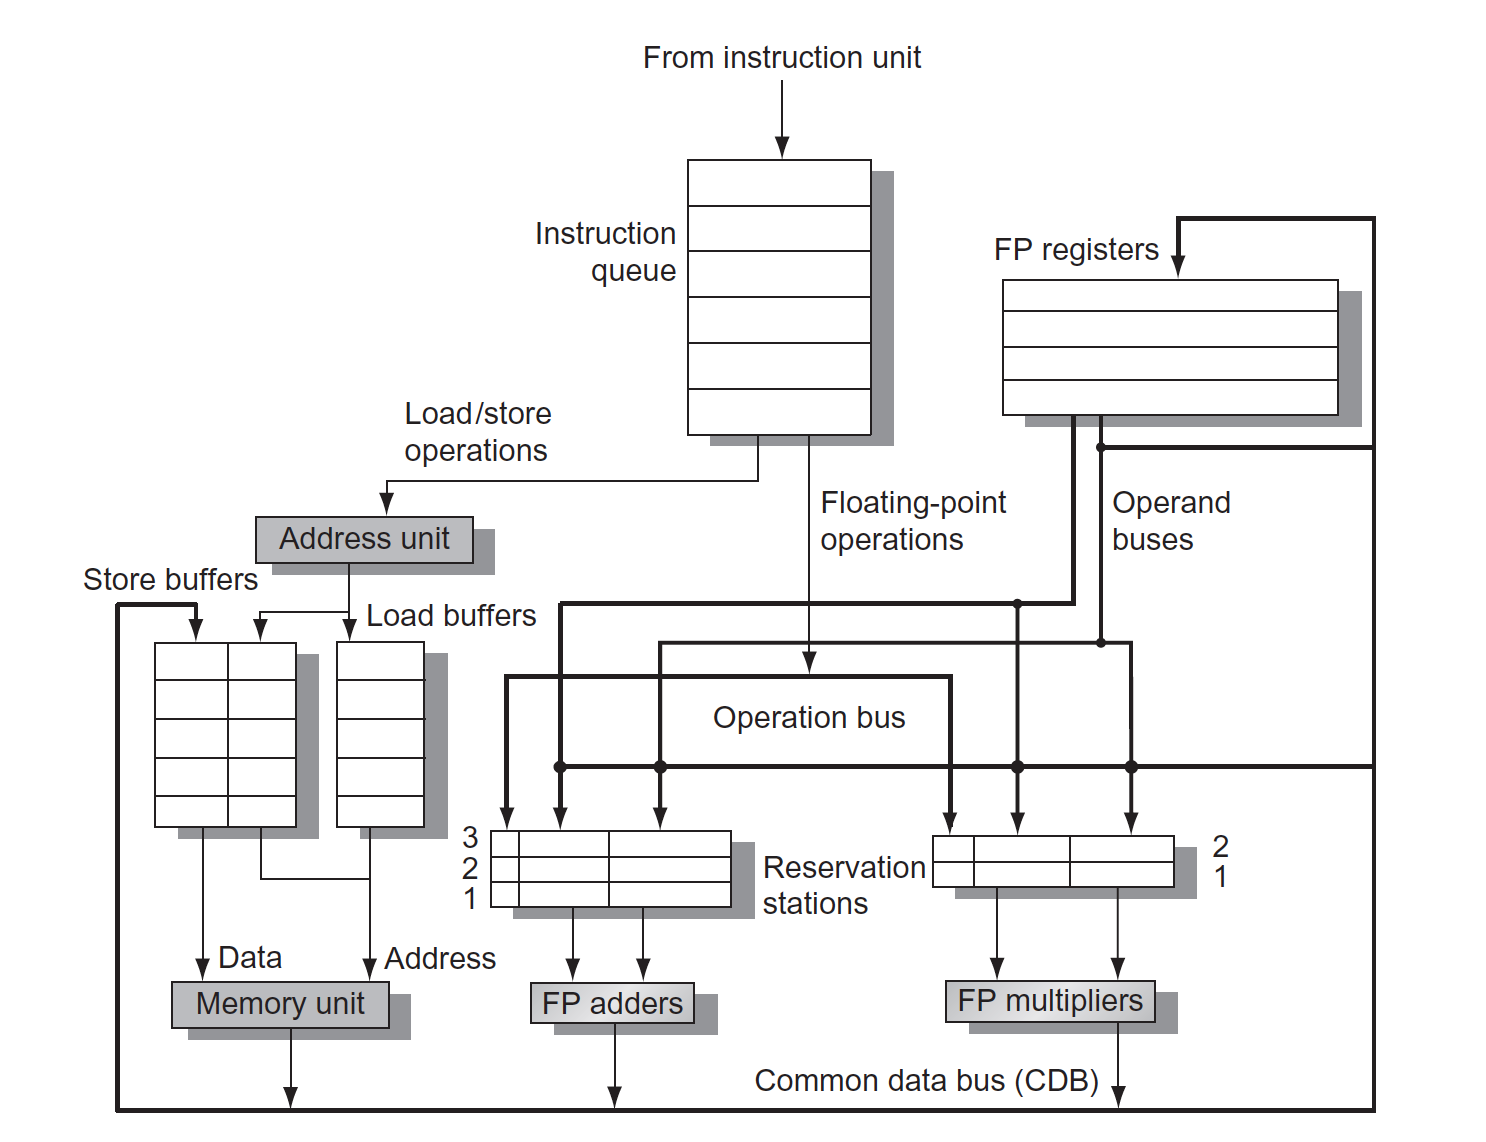
\includegraphics[width=0.75\textwidth]{./images/tomas/tomas.png}	
	\cprotect\caption{Basic structure of a FP unit using Tomasulo’s algorithm}
	\label{fig:tom1}
\end{figure}


As you can see in figure 1, in Tomasulo's algorithm, there is an "instruction queue," in which instructions are stored in FIFO order. We also have a "Reservation Stations" component in this architecture. A reservation station (RS) buffers the operands of fetched instructions waiting to issue, and it will fetches and buffer an operand as soon as it becomes available.

Reservation stations are associated with functional units. As instructions are issued, the register specifiers for pending operands are renamed to the names of the RS, and each instruction identifies RSs which provide its inputs, so they won't need to read their operand from registers.
In addition, results are passed to functional units directly from RSs, thus providing distributed hazard detection, execution control, and better performance since there is no need to read values directly from registers.

Each RS has seven fields:

\begin{itemize}
	\item $Q_P$: Instruction's operation.
	\item $Q_j, Q_k$: The number of RSs that will produce the operands. If operands are already available, the value will be zero.
	\item $V_j, V_k$: The value of operands.
	\item $A$: Value of immediate field or effective address.
	\item $Busy$: Indicates if the RS is in use.
\end{itemize}

Also, each register has a $Q_i$ field which holds the identifier of RS that contains the operation whose result should be stored in this register. If there is no such operation, the value will be zero.

Note that when successive writes to a register happen, only the last one is used to update the register value.

In order to pass operands directly from RSs, the Tomasulo scheme uses a "Common Data Bus" or "CDB," which allows all units waiting for an operand to be loaded simultaneously.

We also have load and store buffers in this architecture that hold data or addresses coming from and going to memory and behave almost exactly like reservation stations.

Load buffers have three functions:
\begin{enumerate}
	\item Holding components of the effective address until it is computed
	\item Tracking outstanding loads that are waiting on the memory
	\item Holding the results of completed loads 
\end{enumerate}

Store buffers also have three functions:
\begin{enumerate}
	\item Holding components of the effective address until it is computed
	\item Holding the destination memory addresses of outstanding stores that are waiting for the data	value to store
	\item Holding the address and value to store until the memory unit is available.
\end{enumerate}


Now we can explain the instruction lifecycle in Tomasulo's algorithm in three steps:

\begin{enumerate}
	\item Issue:
	
	The next instruction is fetched from the instruction queue. If there is any matching RS available, the instruction and its operands  (if available) are issued into that RS. If there is no empty RS, the instruction issue will be stalled.
	If the instruction operands are not available, we store the identifier of RSs that will produce the operands. This step is renaming operands, eliminating WAR and WAW hazards.
	
	\item Execute:
	
	The CDB is monitored until all operands are available. RAW hazards are avoided by delaying instruction execution until the operands are available. When all operands become available, the instruction can be executed at the corresponding functional unit.
	
	Loads and stores require a two-step execution process. In the first step, the effective address is computed. After that, loads can be executed as soon as the memory unit is available. Stores in the store buffer need to wait for the value to be stored before being sent to the memory unit.
	
	\item Write result:
	
	Write result (and source) on CDB after finishing execution. This will result in the value being written in all registers and RSs waiting for this result.
	
\end{enumerate}


Example:

\begin{figure}[H]
	\centering
	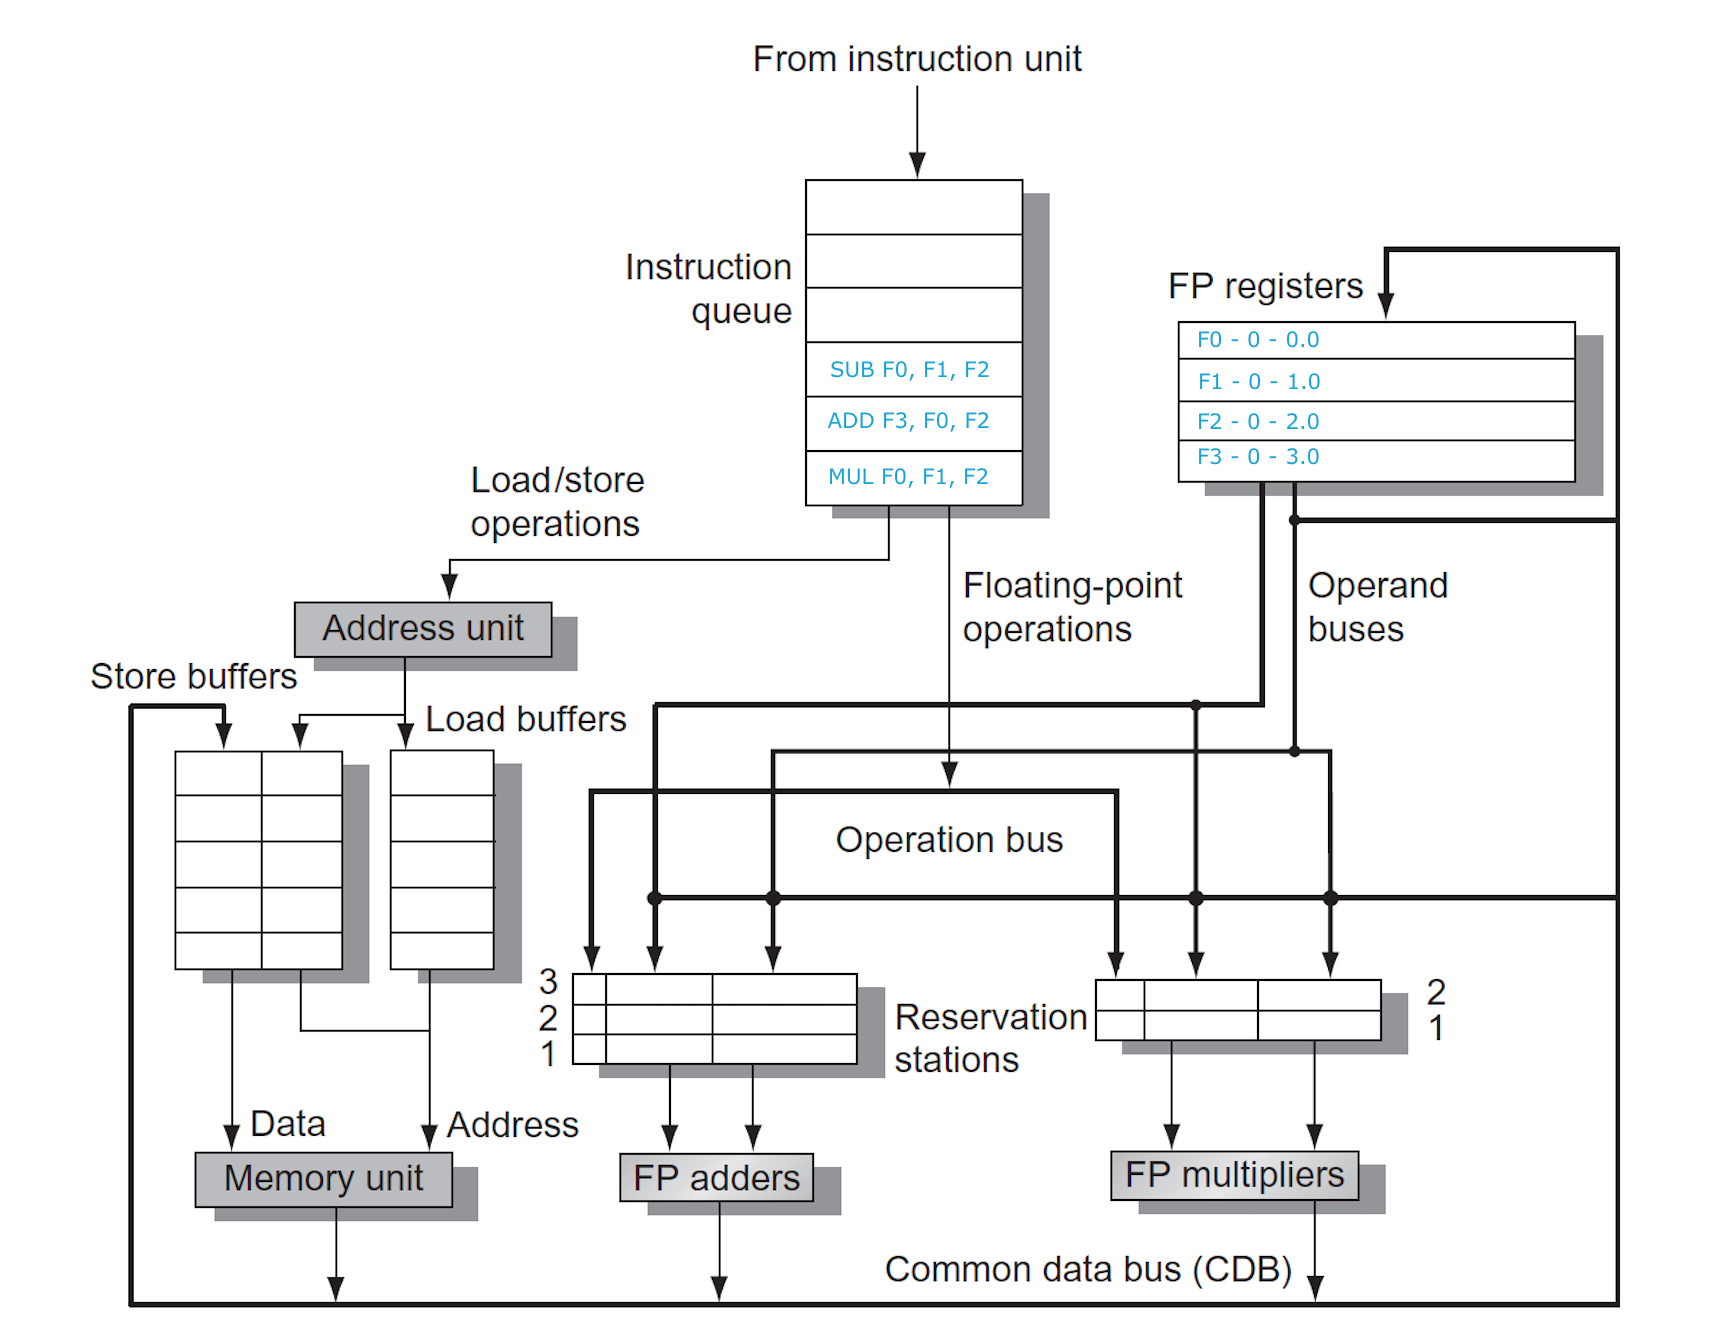
\includegraphics[width=0.7\textwidth]{./images/tomas/e1.png}	
	\cprotect\caption{stage 1}
	\label{fig:tom2}
\end{figure}


Assume following code:

\begin{lstlisting}[style=CStyle]
	MUL F0, F1, F2
	ADD F3, F0, F2
	SUB F0, F1, F2
\end{lstlisting}


The initial state is shown in Figure \ref{fig:tom2}.

First, the MUL instruction is issued with its operands in reservation station 1 of the multiplication unit. We call this reservation station MUL1. Notice the $Q_i$ field of register F0 is set to MUL1.

After that, the ADD instruction is issued in reservation station 1 of the addition unit called ADD1. Since one of its operands is not available yet, it is issued with the identifier of RS that provides its operand, MUL1. Notice the $Q_i$ field of register F3 is set to ADD1. (Figure \ref{fig:tom3})

This is how the register renaming is performed. We have renamed F0 to MUL1, and ADD instruction is no longer waiting for F0 to become available. Instead, it will wait until the MUL1 result is available on CDB, thus eliminating name dependencies. 

\begin{figure}[H]
	\centering
	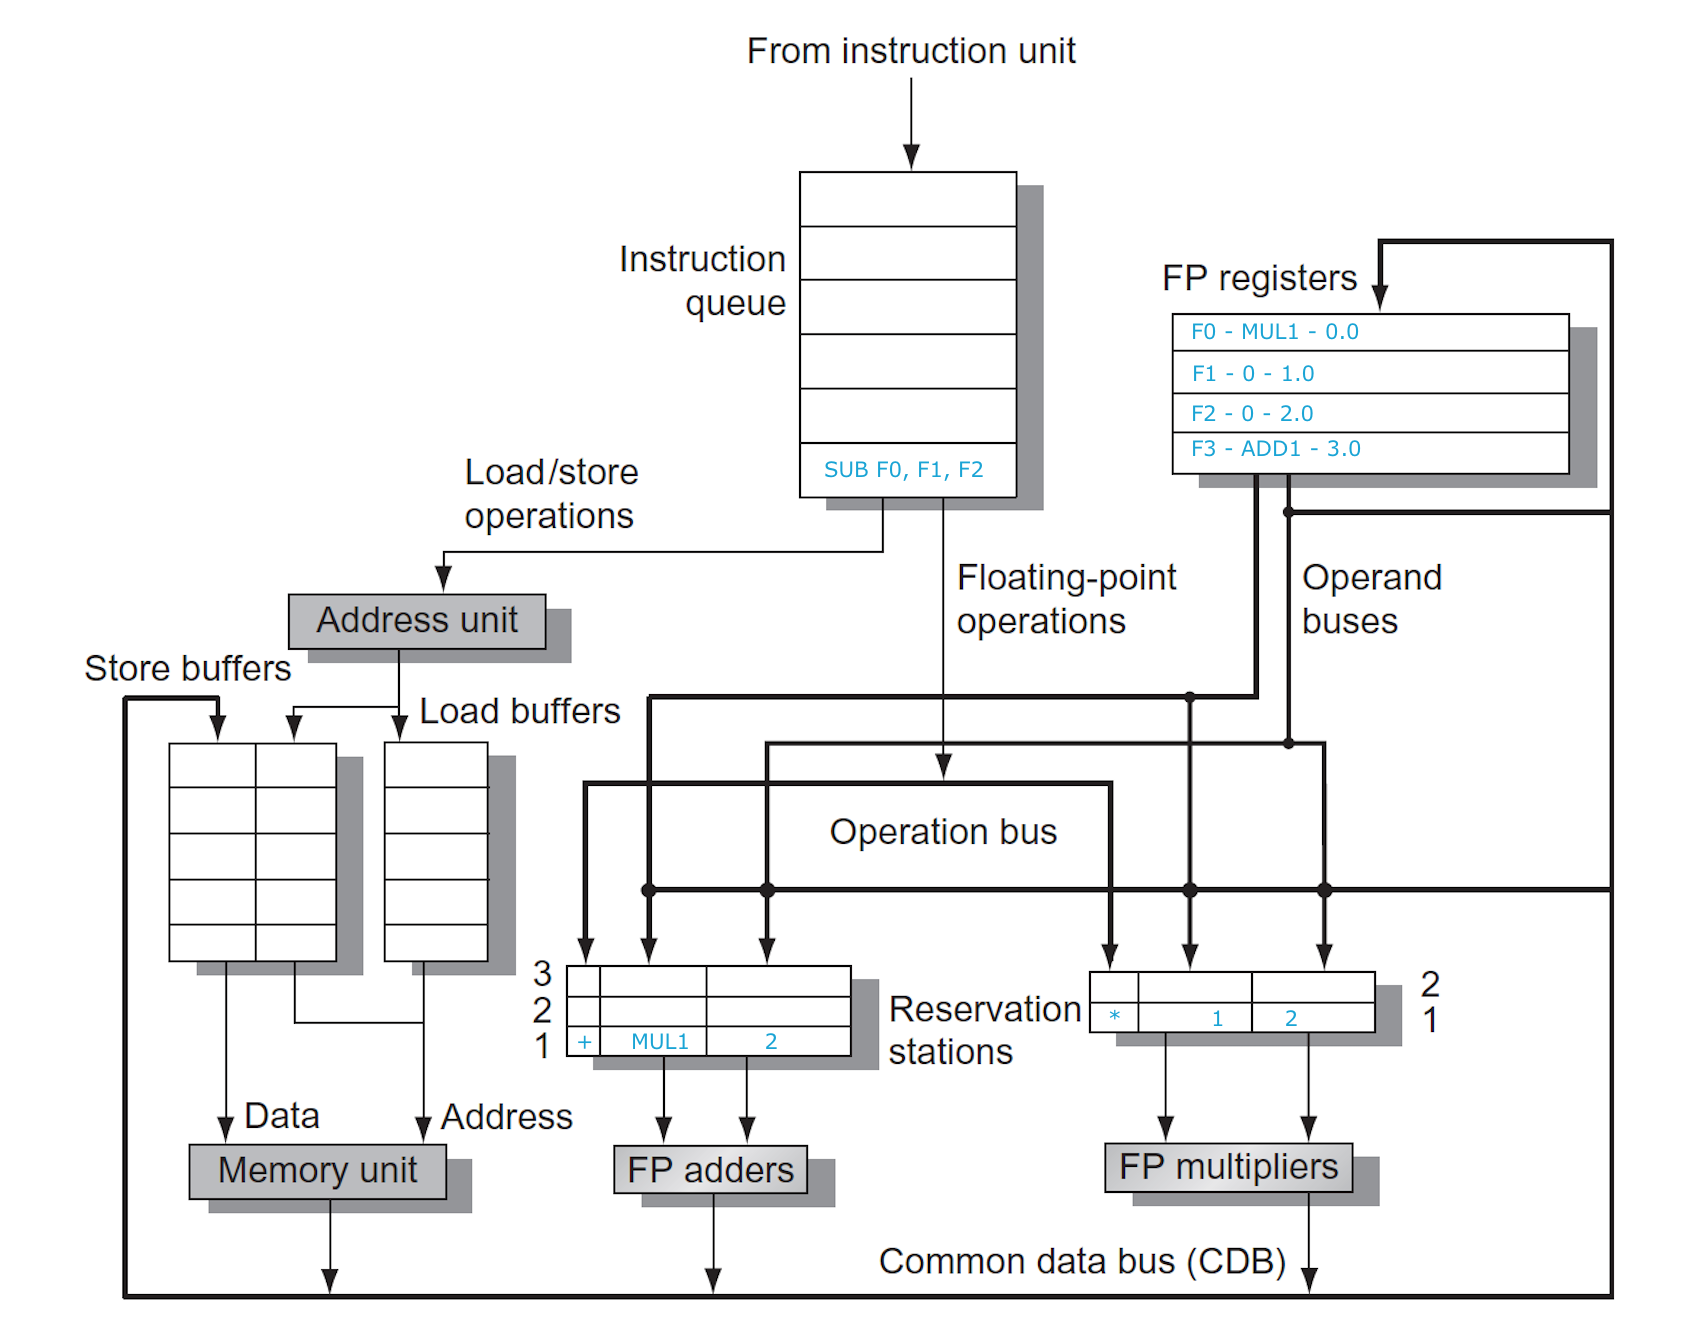
\includegraphics[width=1\textwidth]{./images/tomas/e2.png}	
	\cprotect\caption{stage 2}
	\label{fig:tom3}
\end{figure}


Assume that next, the SUB instruction is issued with its operands in RS 2 of the addition unit, which we will call ADD2. The $Q_i$ field of F0 is now set to ADD2. This means that result of MUL instruction is never written to the register file. (Figure \ref{fig:tom4})

\begin{figure}[H]
	\centering
	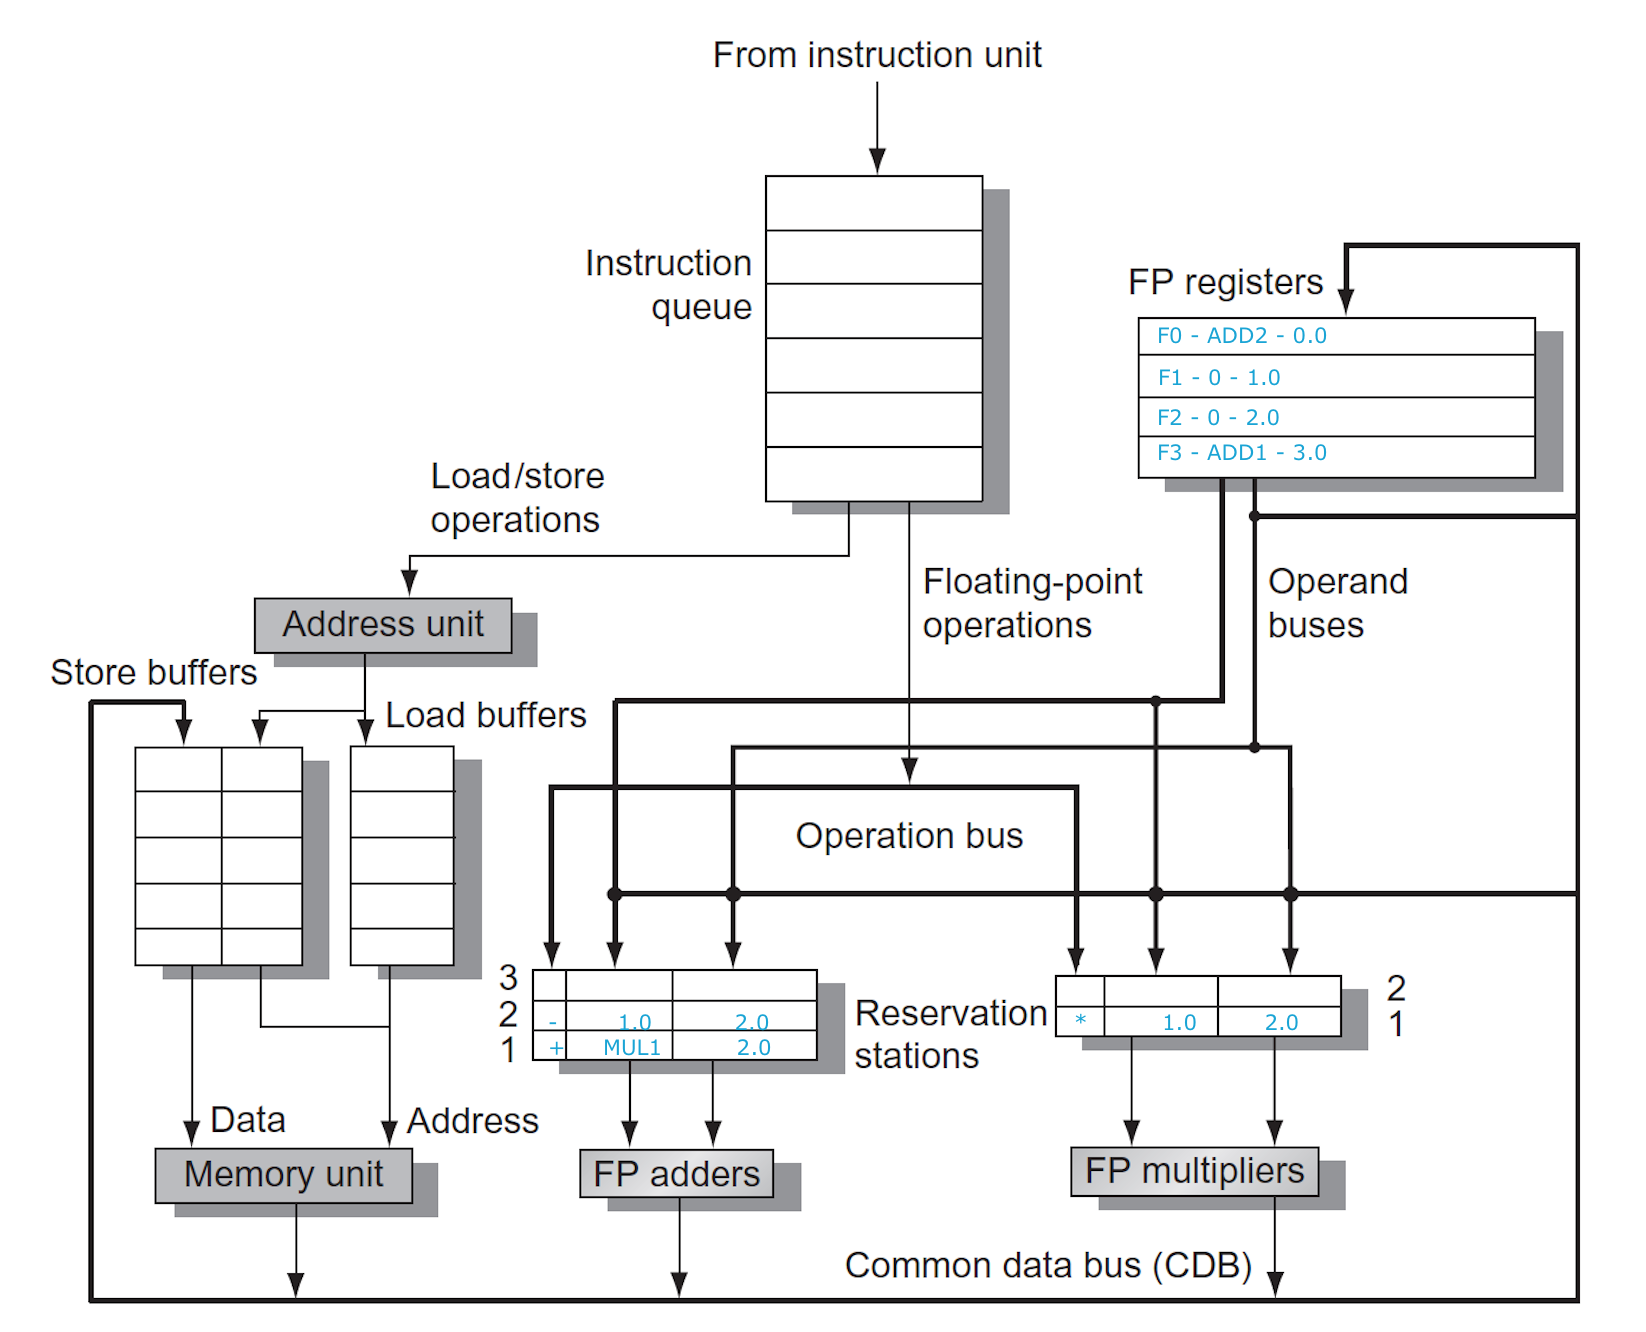
\includegraphics[width=1\textwidth]{./images/tomas/e3.png}	
	\cprotect\caption{stage 3}
	\label{fig:tom4}
\end{figure}


Now any of MUL or SUB instructions can be executed. The state of RSs and registers after execution of these two instructions is shown in Figure \ref{fig:tom5}. 

\begin{figure}[H]
	\centering
	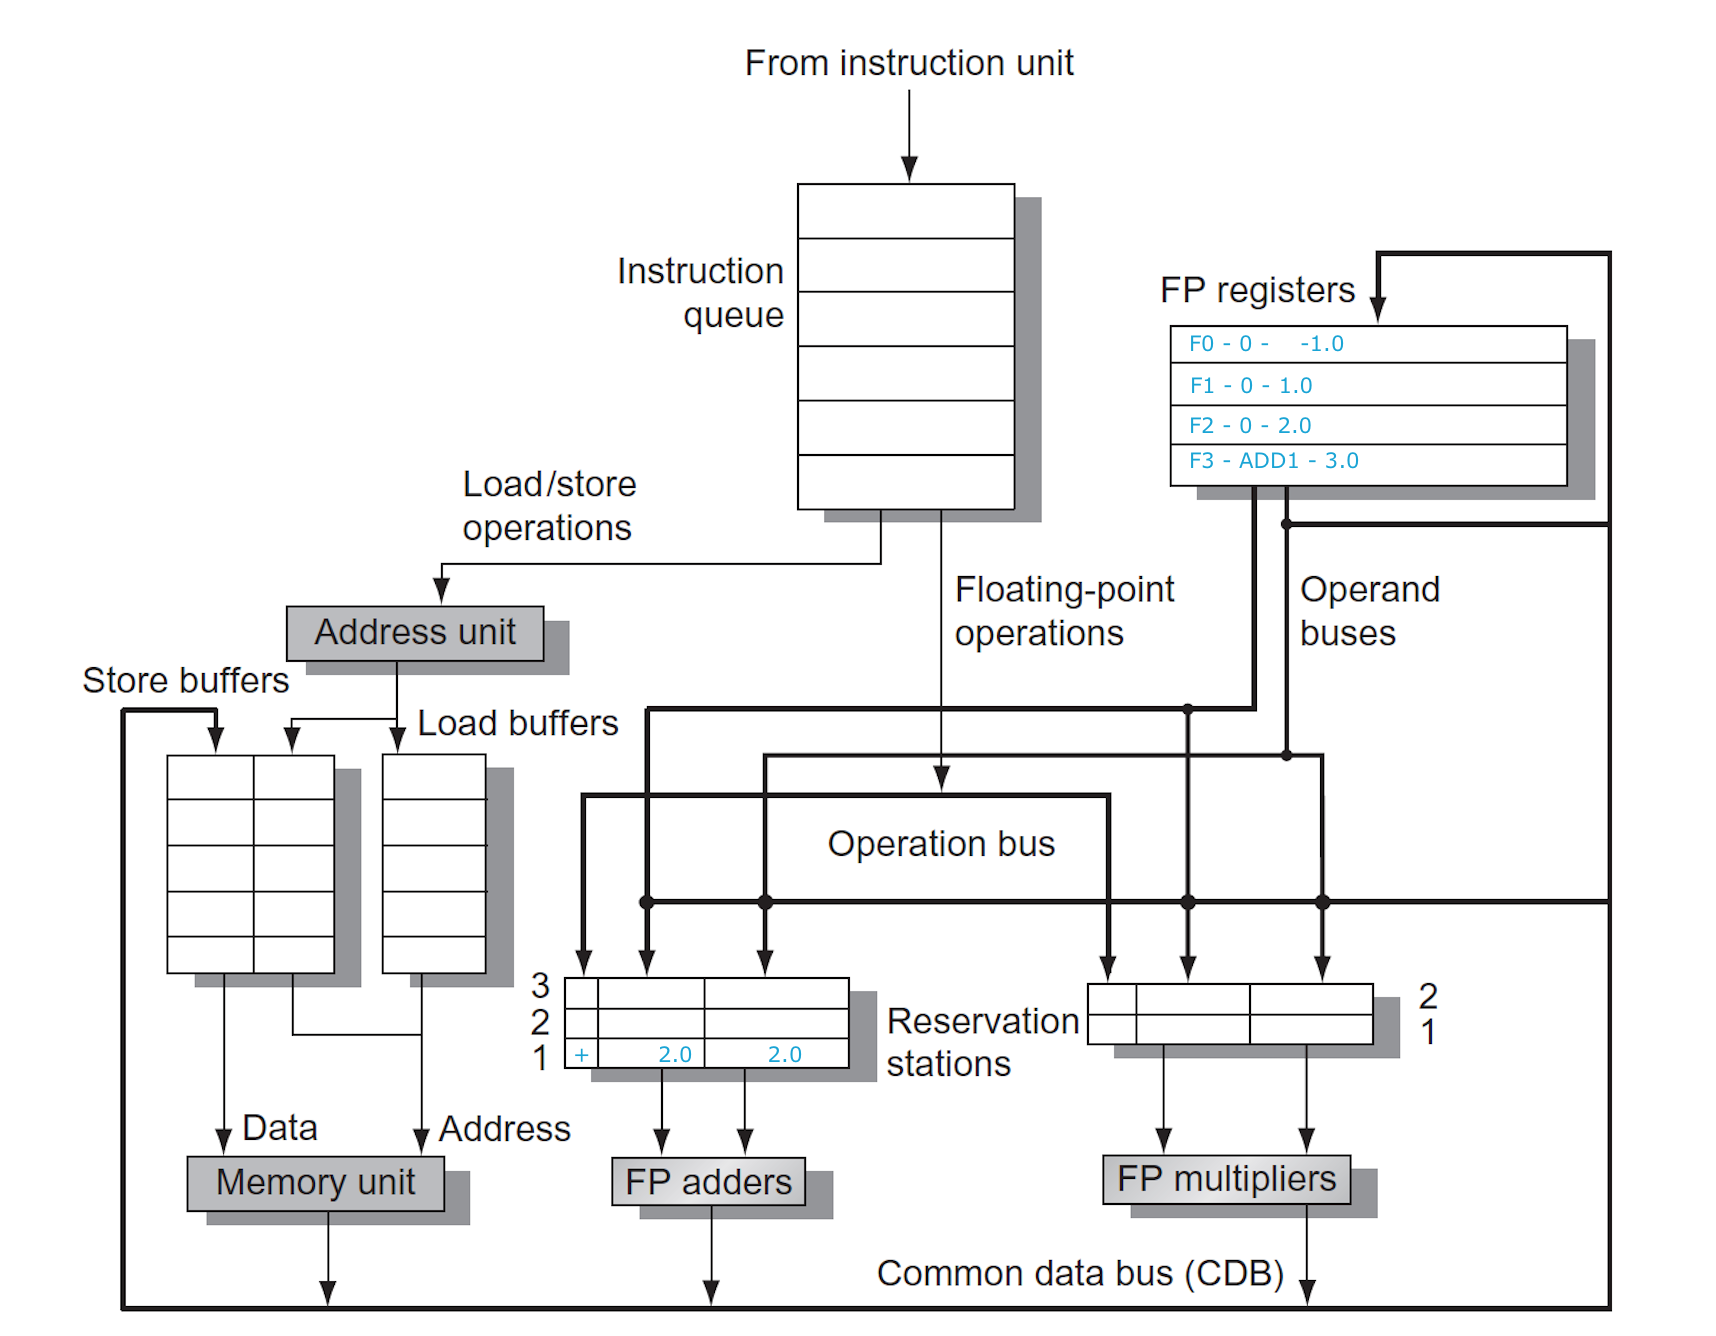
\includegraphics[width=1\textwidth]{./images/tomas/e4.png}	
	\cprotect\caption{stage 4}
	\label{fig:tom5}
\end{figure}


Since MUL1 is executed, all operands of ADD instruction are ready and can also be executed. You can see the final state in Figure \ref{fig:tom6}.

\begin{figure}[H]
	\centering
	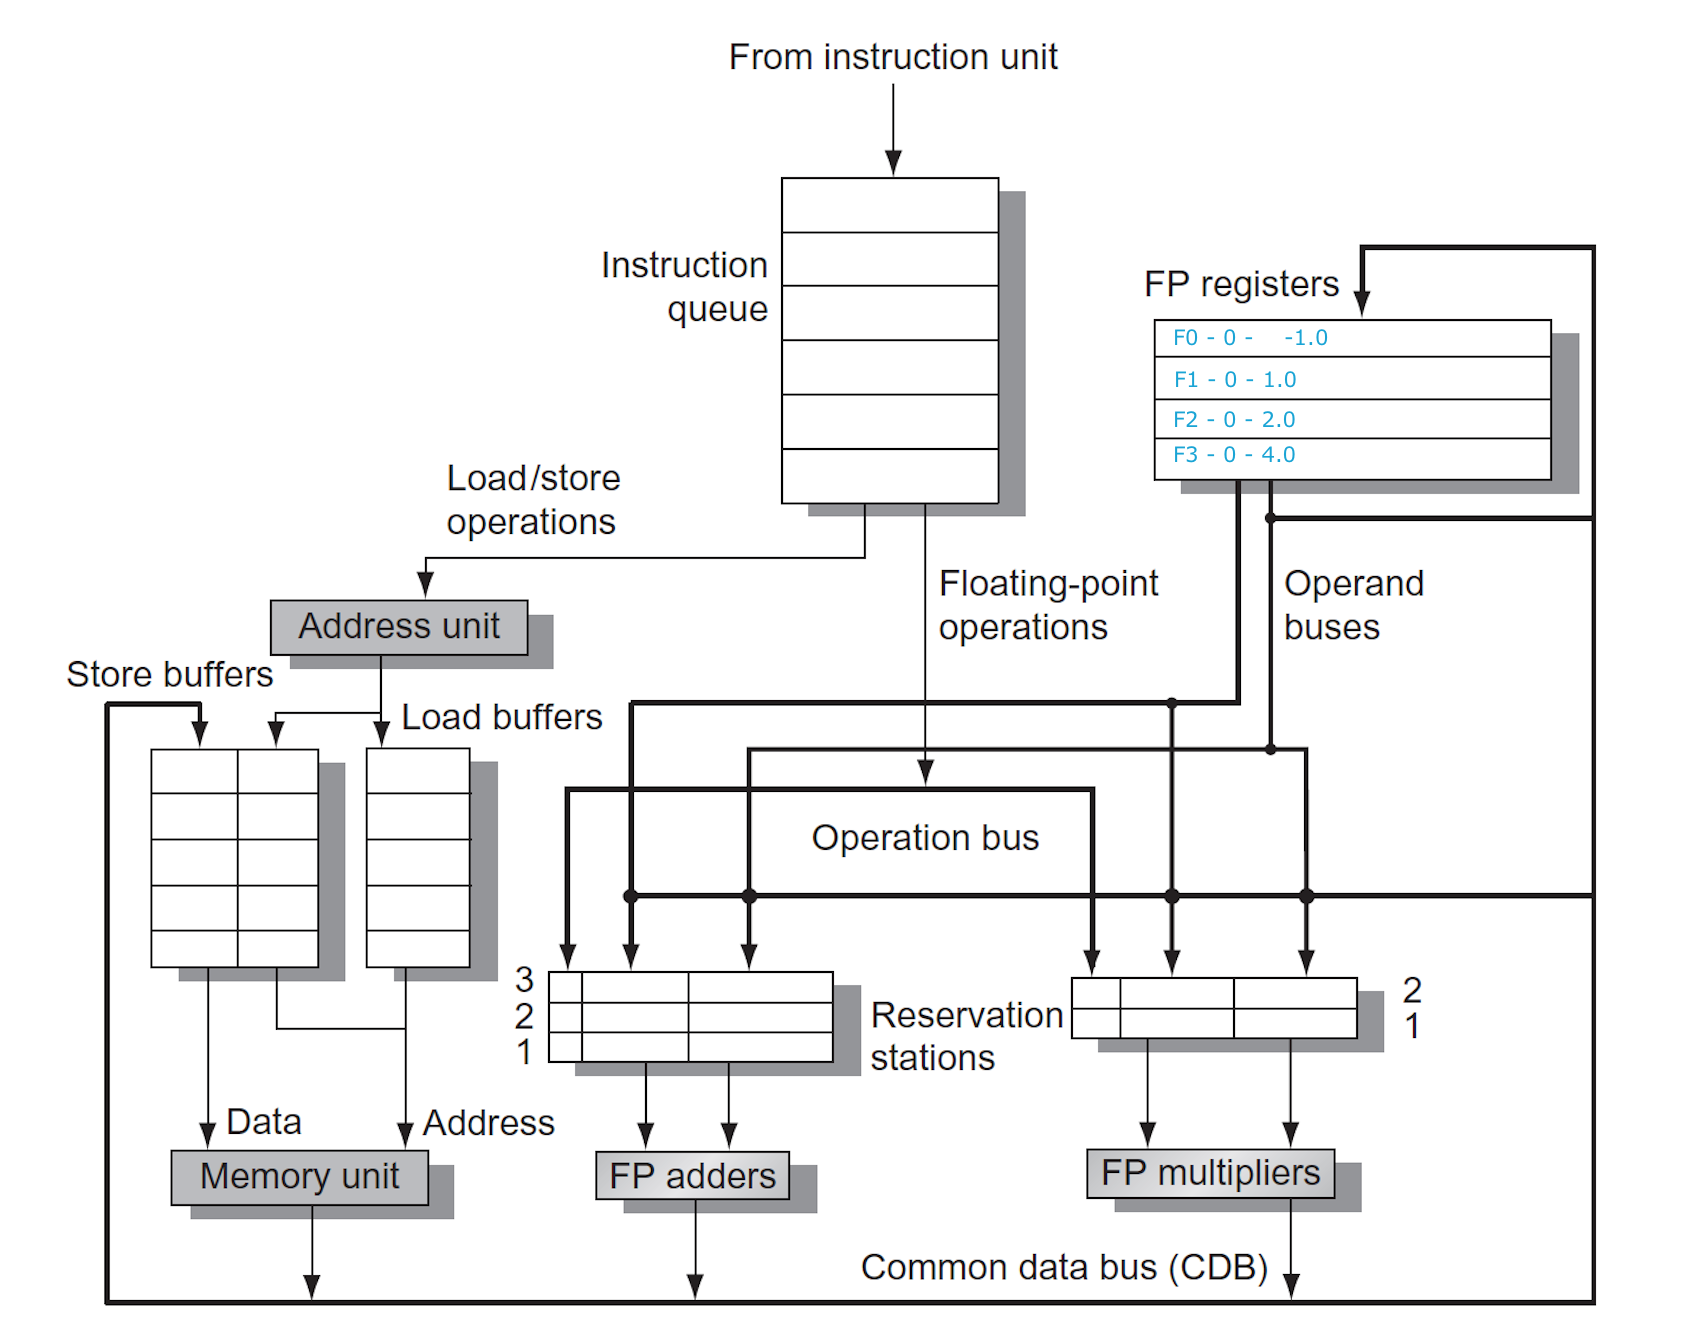
\includegraphics[width=1\textwidth]{./images/tomas/e5.png}	
	\cprotect\caption{stage 5}
	\label{fig:tom6}
\end{figure}


The drawback of Tomasulo is its complexity. Also, CDB can be a single point of failure. This issue can be avoided by using multiple CDBs.

Tomasulo can also be extended to support speculation. In order to do this, bypassing the result among instructions and the actual completion of an instruction need to be separated. This allows instructions to execute
out of order but to force them to commit in order and prevent any unwanted action until an instruction commits.

One other thing to notice in Tomasulo's Algorithm is that it uses a greedy algorithm to find an execution order of instructions.
The algorithm will not use any subsequent dependence information in this greedy approach. But by using this information, such as dependency chain length, dependants count, slack time, etc., we can improve the algorithm to give us better order for instructions execution.

\nocite{*}

\bibliographystyle{plain}
\bibliography{refs}


% Resources:
% Source book
% Dynamic Scheduling Using Tomasulo's Algorithm https://www.youtube.com/watch?v=y-N0Dsc9LmU
% Dynamic Scheduling Using Tomasulo's Algorithm Example https://www.youtube.com/watch?v=YH2fFu-35L8
% Extending Tomasulo with Memory Accesses https://www.youtube.com/watch?v=eI-xrVbUId
% Tomasulo's paper: An Efficient Algorithm for Exploiting Multiple Arithmetic Units
% https://courses.cs.washington.edu/courses/cse548/02wi/files/pdf/final/Luna-and-Gang.pdf

\newpage

\section{Question Five}

All parts have been run on a machine with this configuration:

\begin{itemize}
	\item CPU Model: Intel Core i9 11980HK
	\item Memory: 32GB DDR4 - 3200 MHz
	\item Operating System: Pop! OS 21.10
	\item Linux Kernel Version: 5.16.11
\end{itemize}

\subsection{A}


\begin{itemize}
	\item 
	Only including important parts of coded needed for explanation:
	\begin{lstlisting}[style=CStyle]
		//no_branch.cpp
		
		...
		a += p1[i];
		...
	\end{lstlisting}
	
	\begin{lstlisting}[style=CStyle]
		//branch_with_true.cpp
		
		int true_giver(int _i){
			return 1;
		}
		
		if (true_giver(i)) {
			a += p1[i];
		} else {
			a *= p2[i];
		}
	\end{lstlisting}
	
	\begin{lstlisting}[style=CStyle]
		//real_branch.cpp
		...
		c[i] = rand() >= 0;
		...
		if (c_ptr[i]) {
			a += p1[i];
		} else {
			a *= p2[i];
		}
		...
	\end{lstlisting}
	
	As we can see, the \Verb+no_branch.cpp+ simply adds \codeword{p1[i]+} to the \codeword{a} variable. 
	
	The \Verb+branch_wit_true+ has an \codeword{if} statement, but because of \codeword{true_giver} function, only the first part of if which is \codeword{a+=p1[i]} gets executed. 
	
	For the \Verb+real_branch+, we have an if on \codeword{c_ptr[i]} but we can see that each element of \codeword{c}, which is the vector that \codeword{c_ptr} points to, has the value of \codeword{rand() >= 0}, and because \codeword{rand()}  always generates numbers in greater than or equal to $0$, the \codeword{if}'s condition will evaluate to true.
	
	\item
	In the following pictures, you can see the output of \Verb+perf stat+ for of all files:
	
\begin{figure}[H]
	\centering
	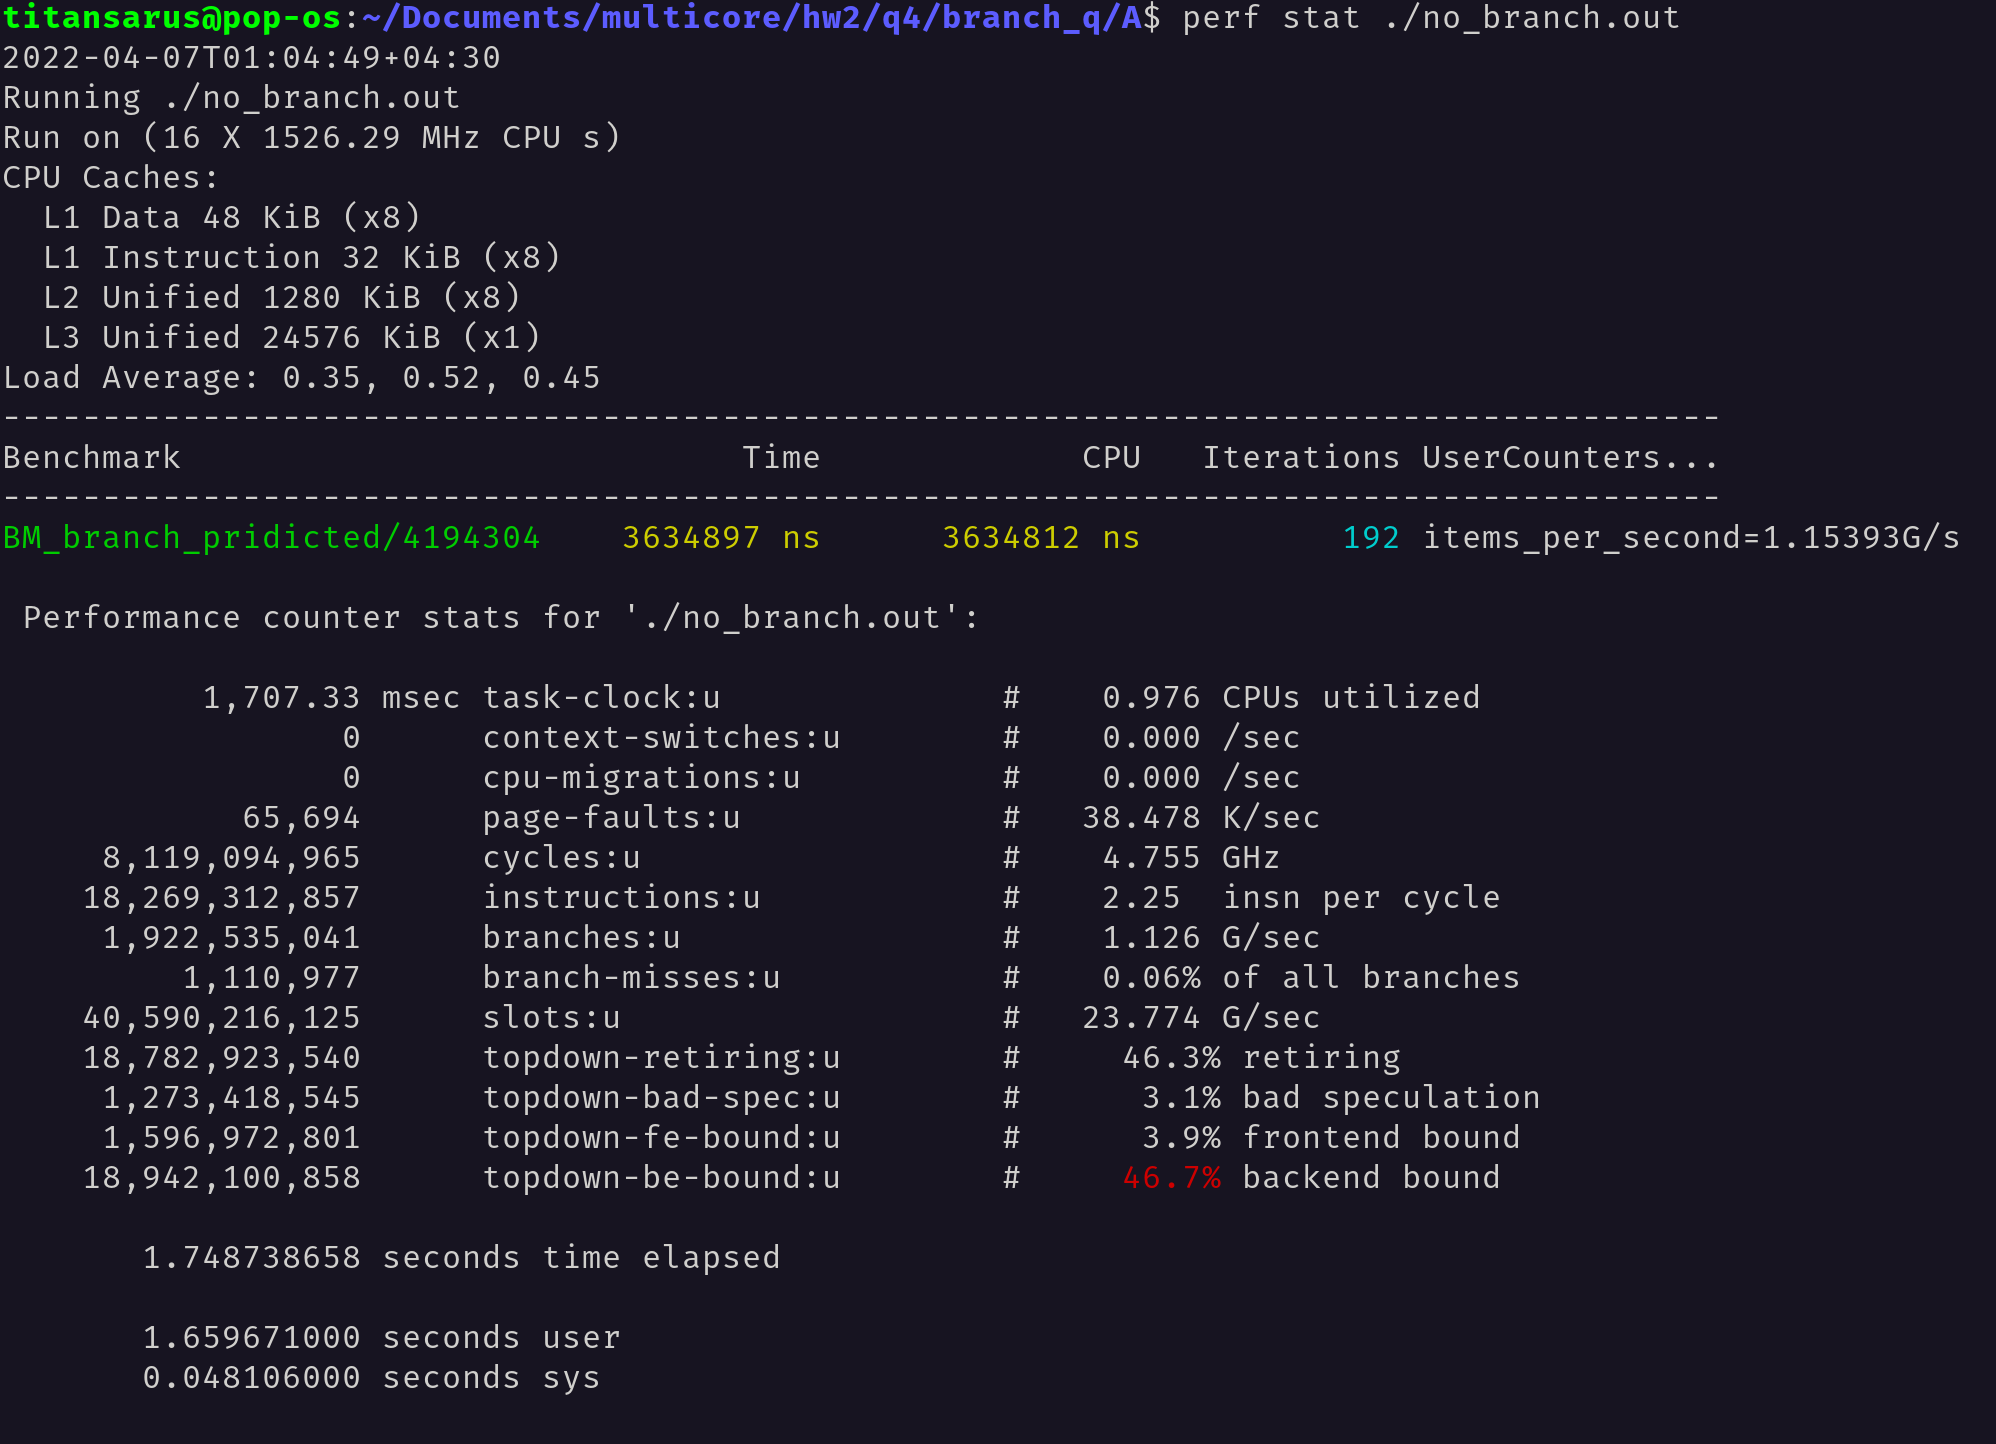
\includegraphics[width=0.8\textwidth]{./images/4A/no-branch.png}	
	\cprotect\caption{\Verb+no_branch.out+}
\end{figure}



\begin{figure}[H]
	\centering
	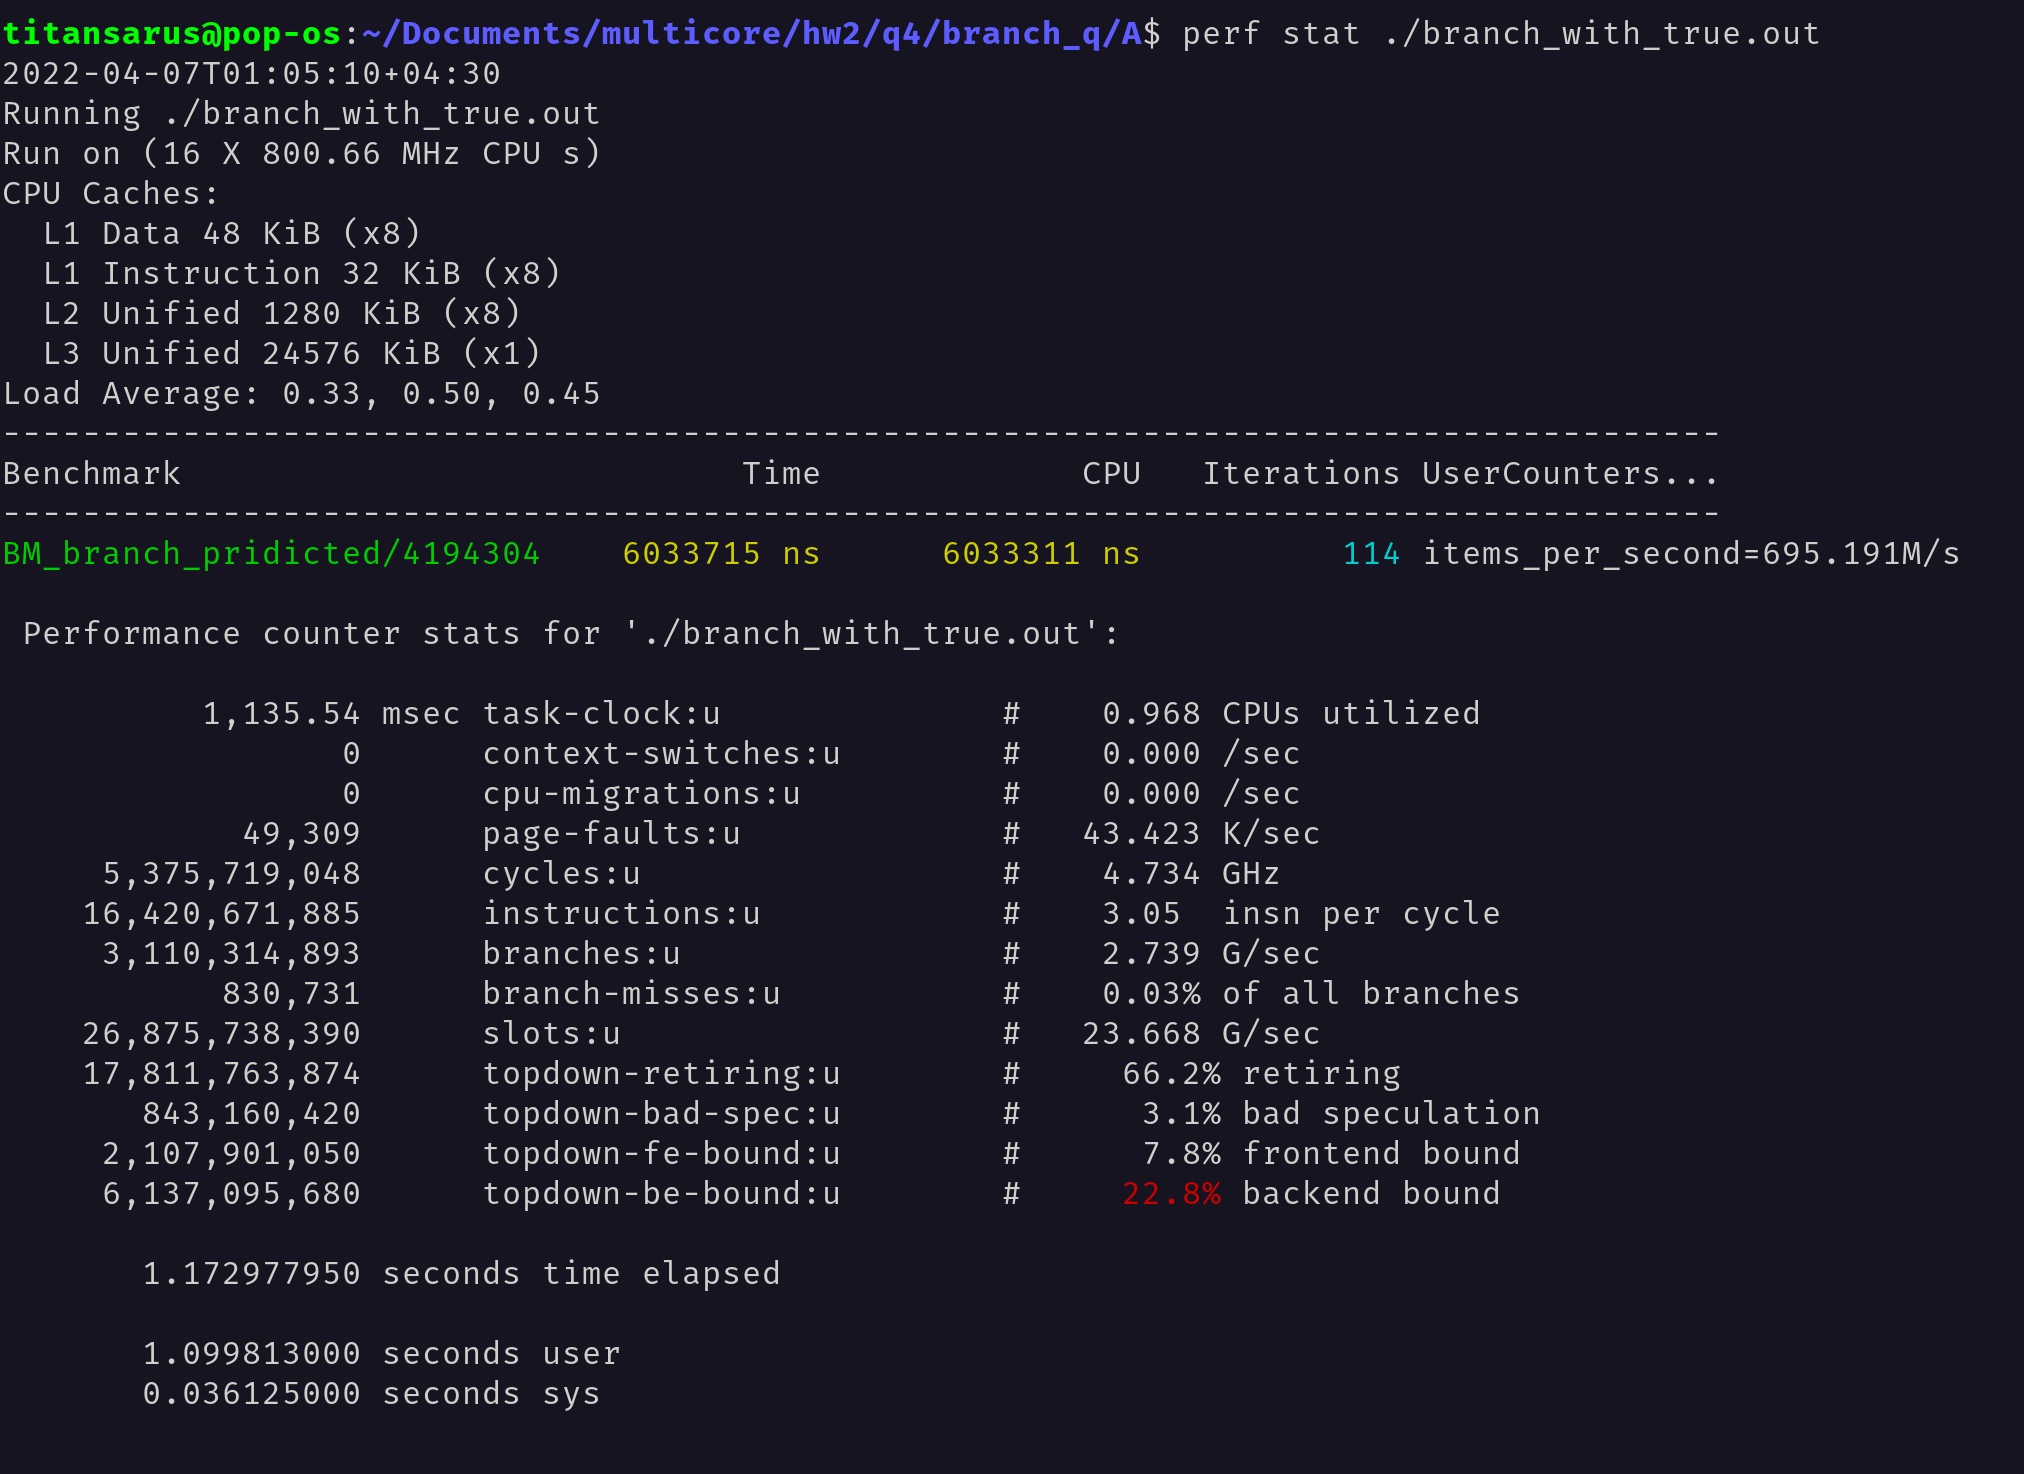
\includegraphics[width=0.8\textwidth]{./images/4A/branch-with-true.png}	
	\cprotect\caption{\Verb+branch_with_true.out+}
\end{figure}

\begin{figure}[H]
	\centering
	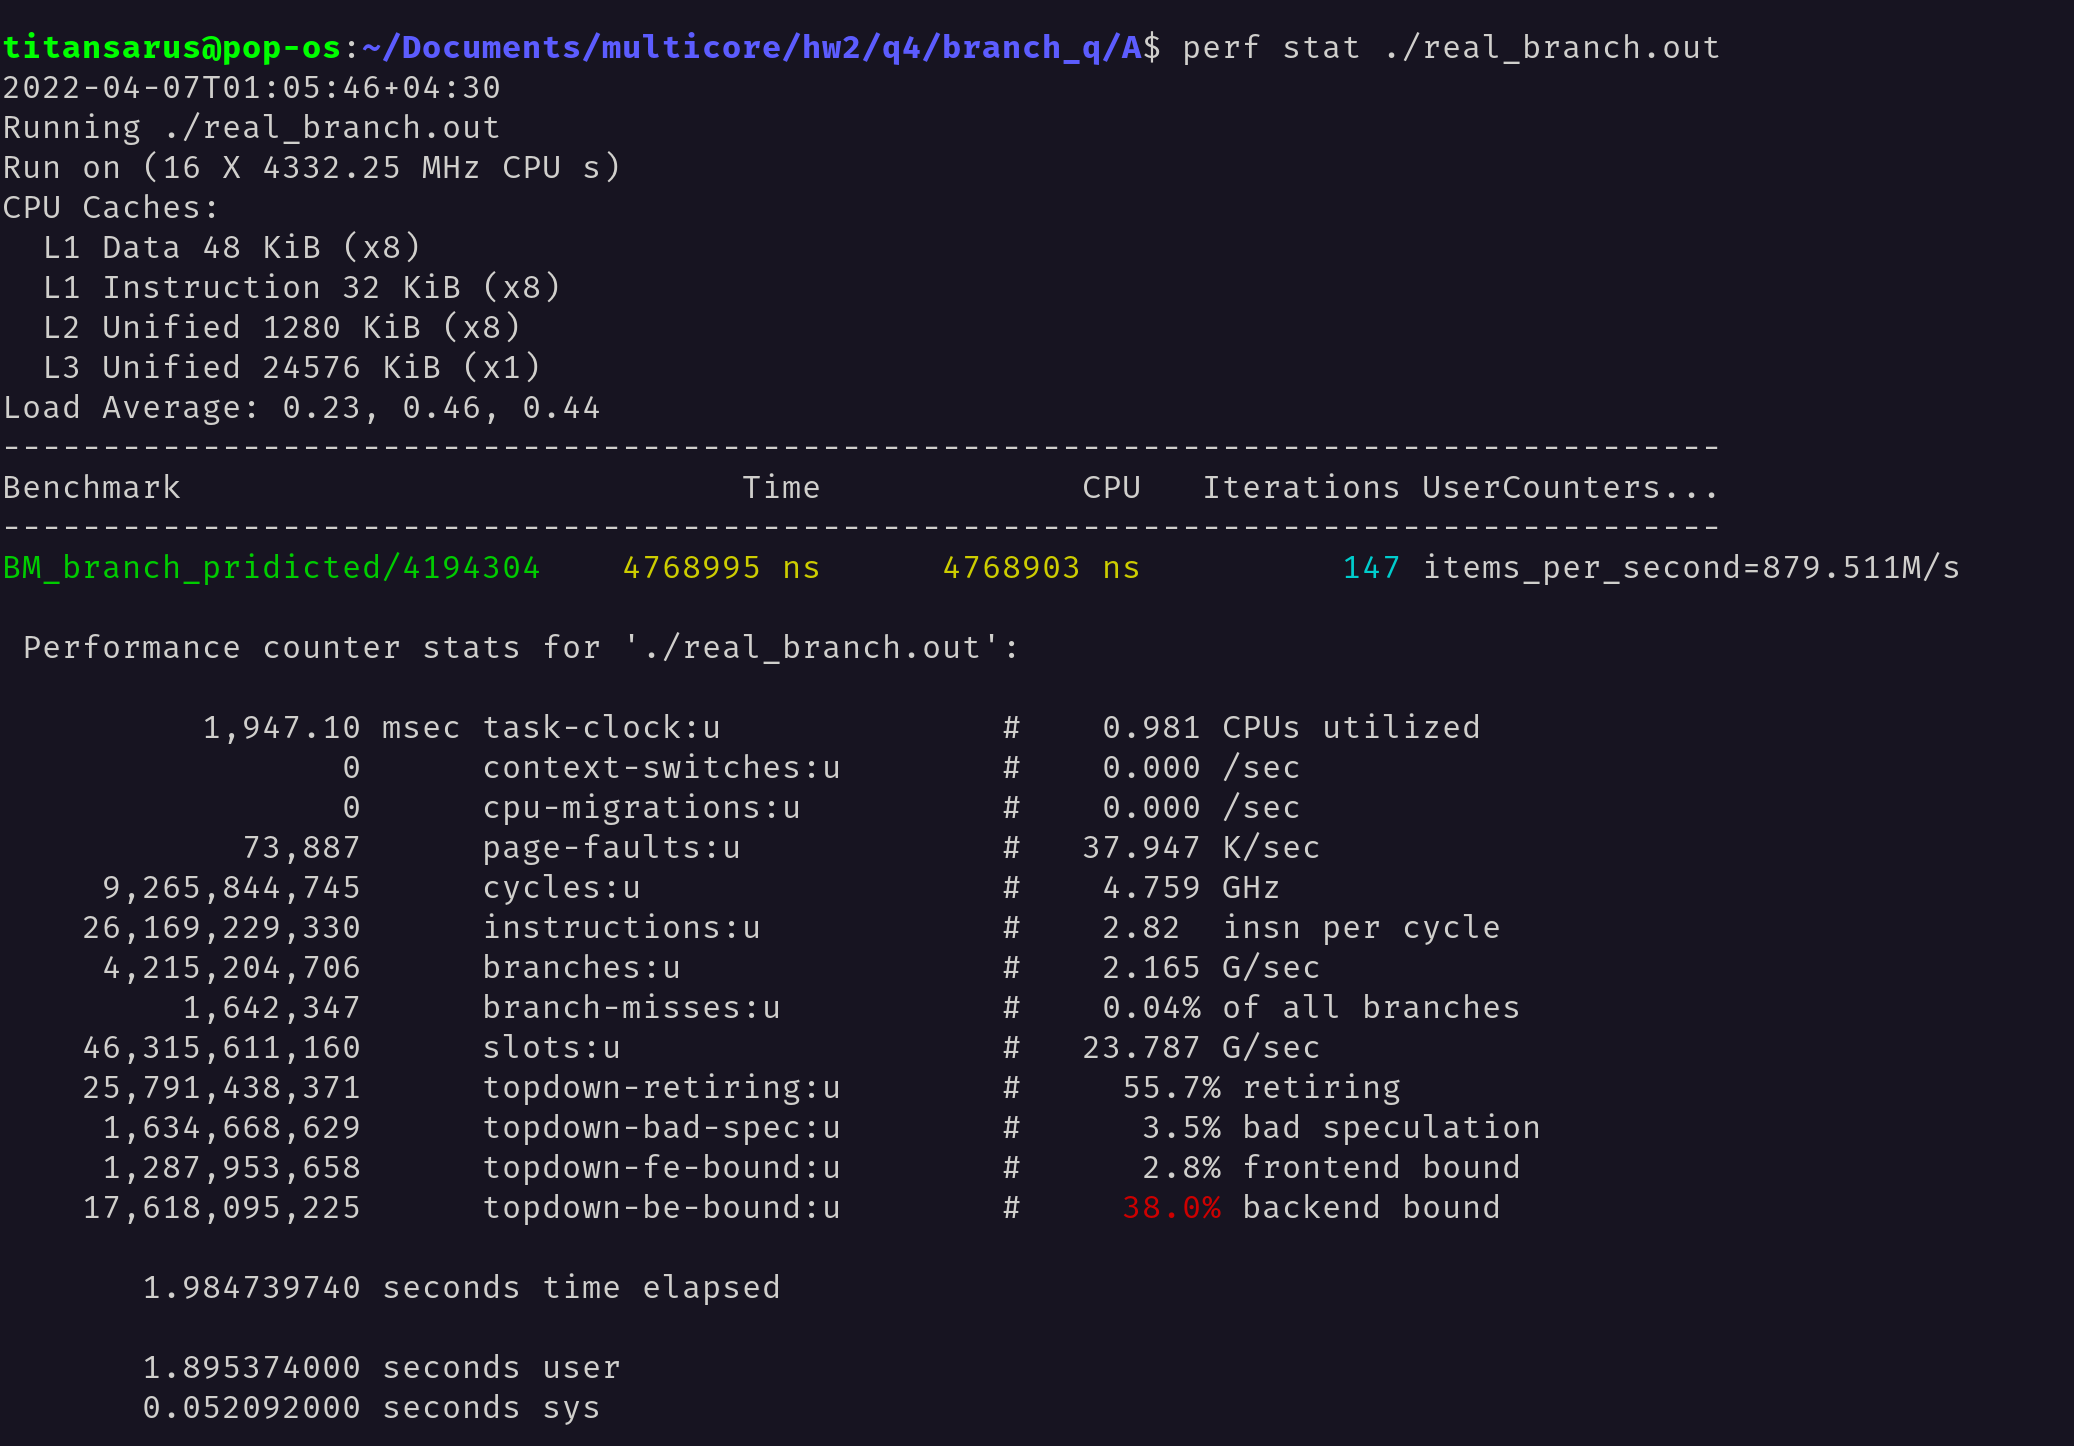
\includegraphics[width=0.8\textwidth]{./images/4A/real-branch.png}	
	\cprotect\caption{\Verb+real_branch.out+}
\end{figure}

\begin{figure}[H]
	\centering
	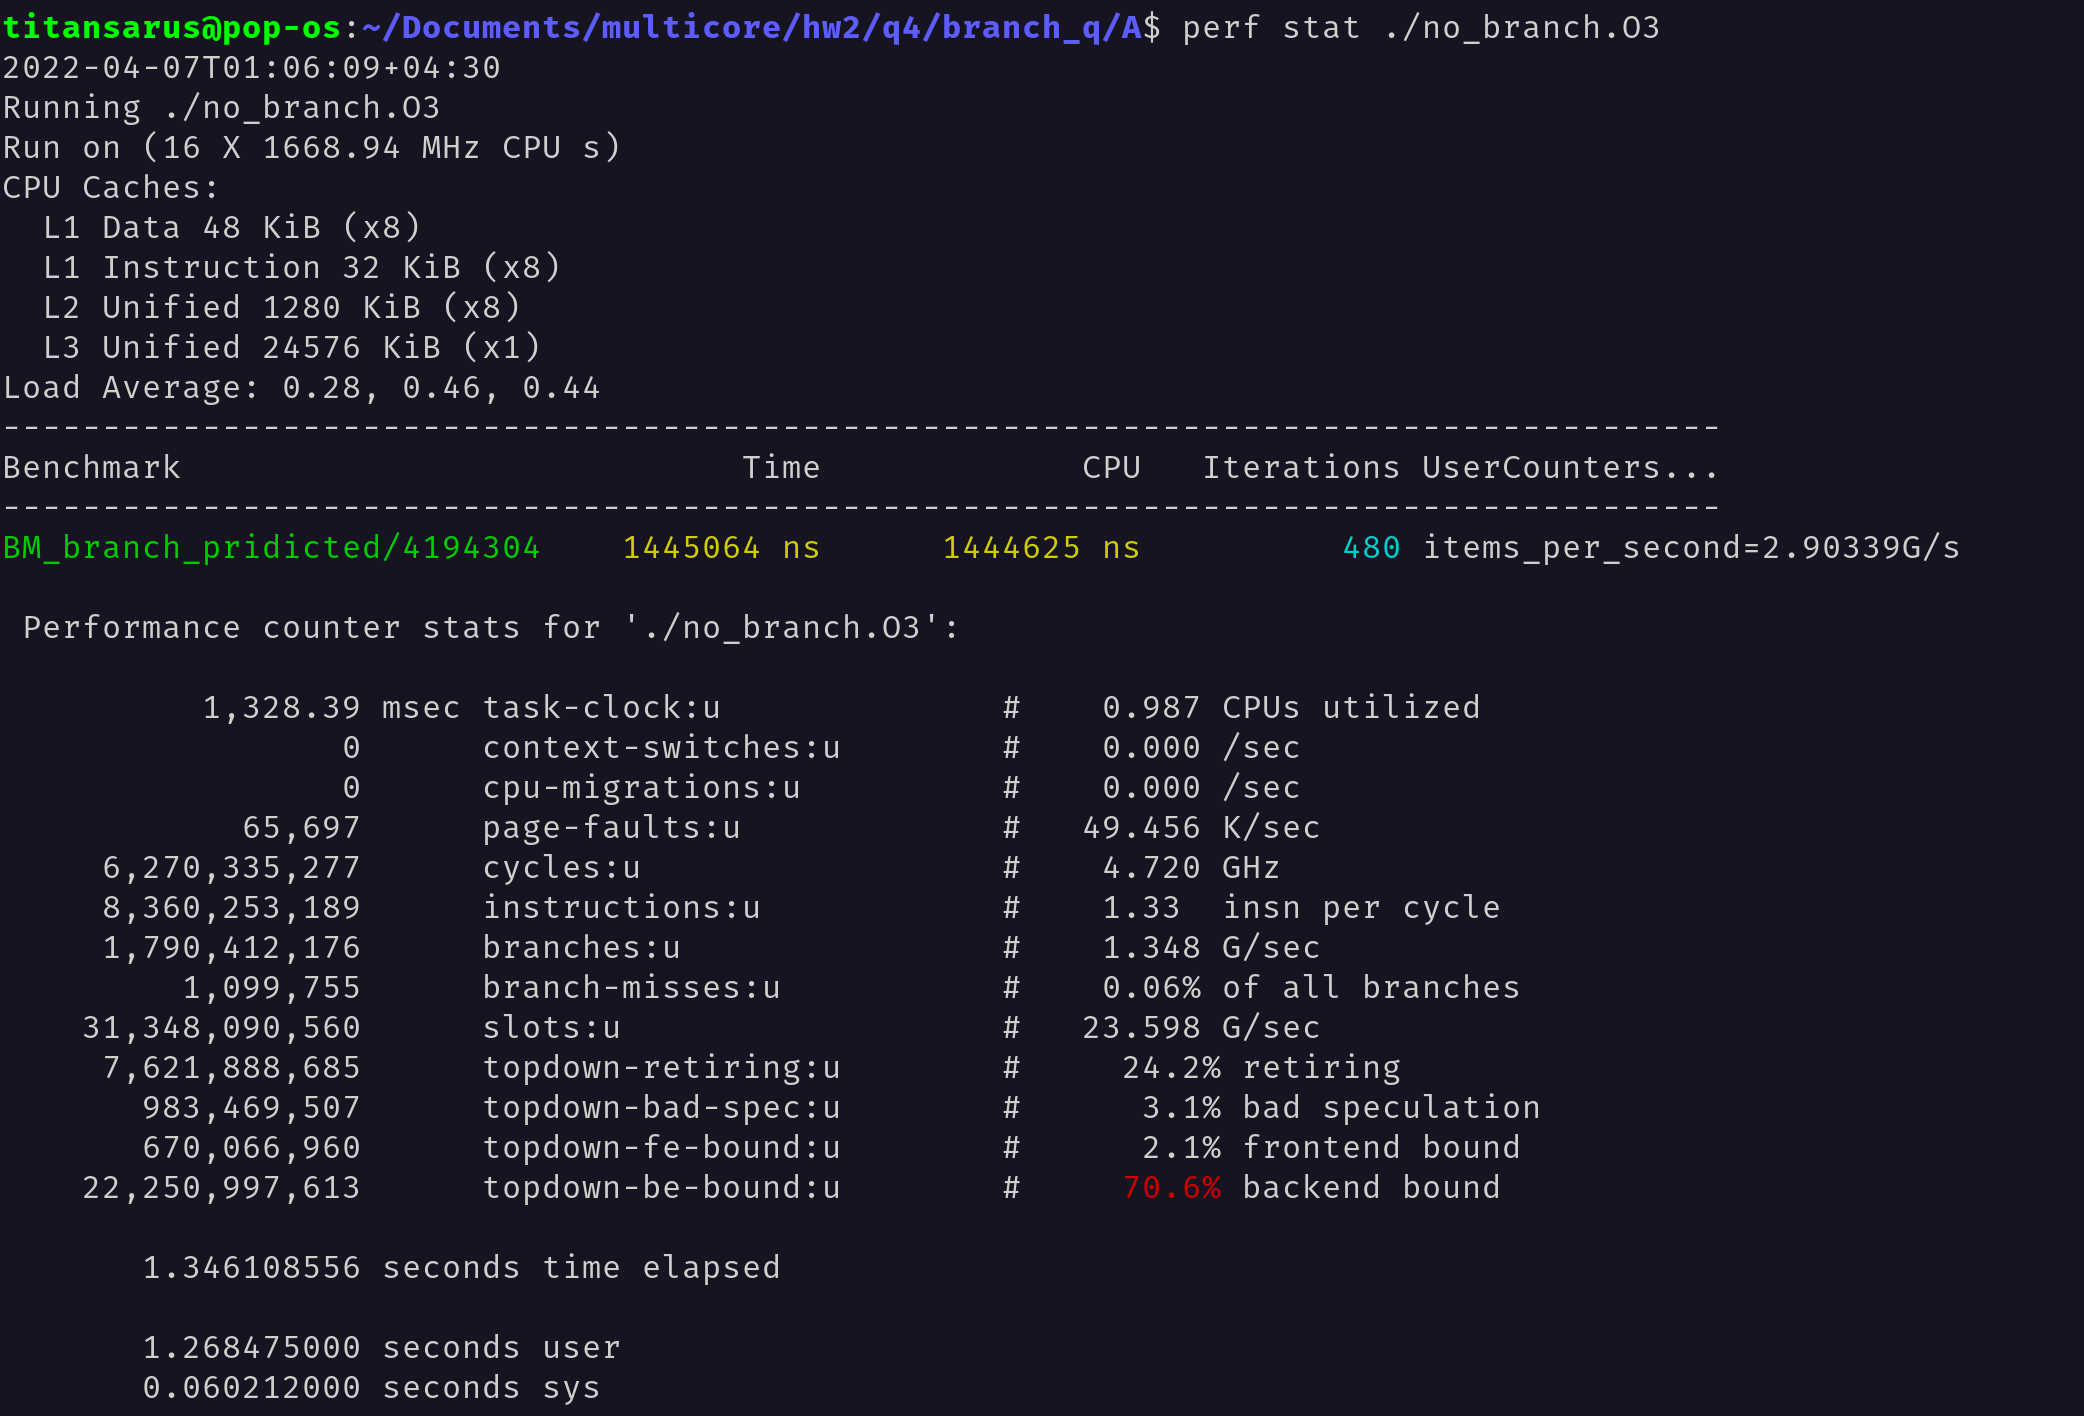
\includegraphics[width=0.8\textwidth]{./images/4A/no-branch-o3.png}	
	\cprotect\caption{\Verb+no_branch.O3+}
\end{figure}
			

\begin{figure}[H]
	\centering
	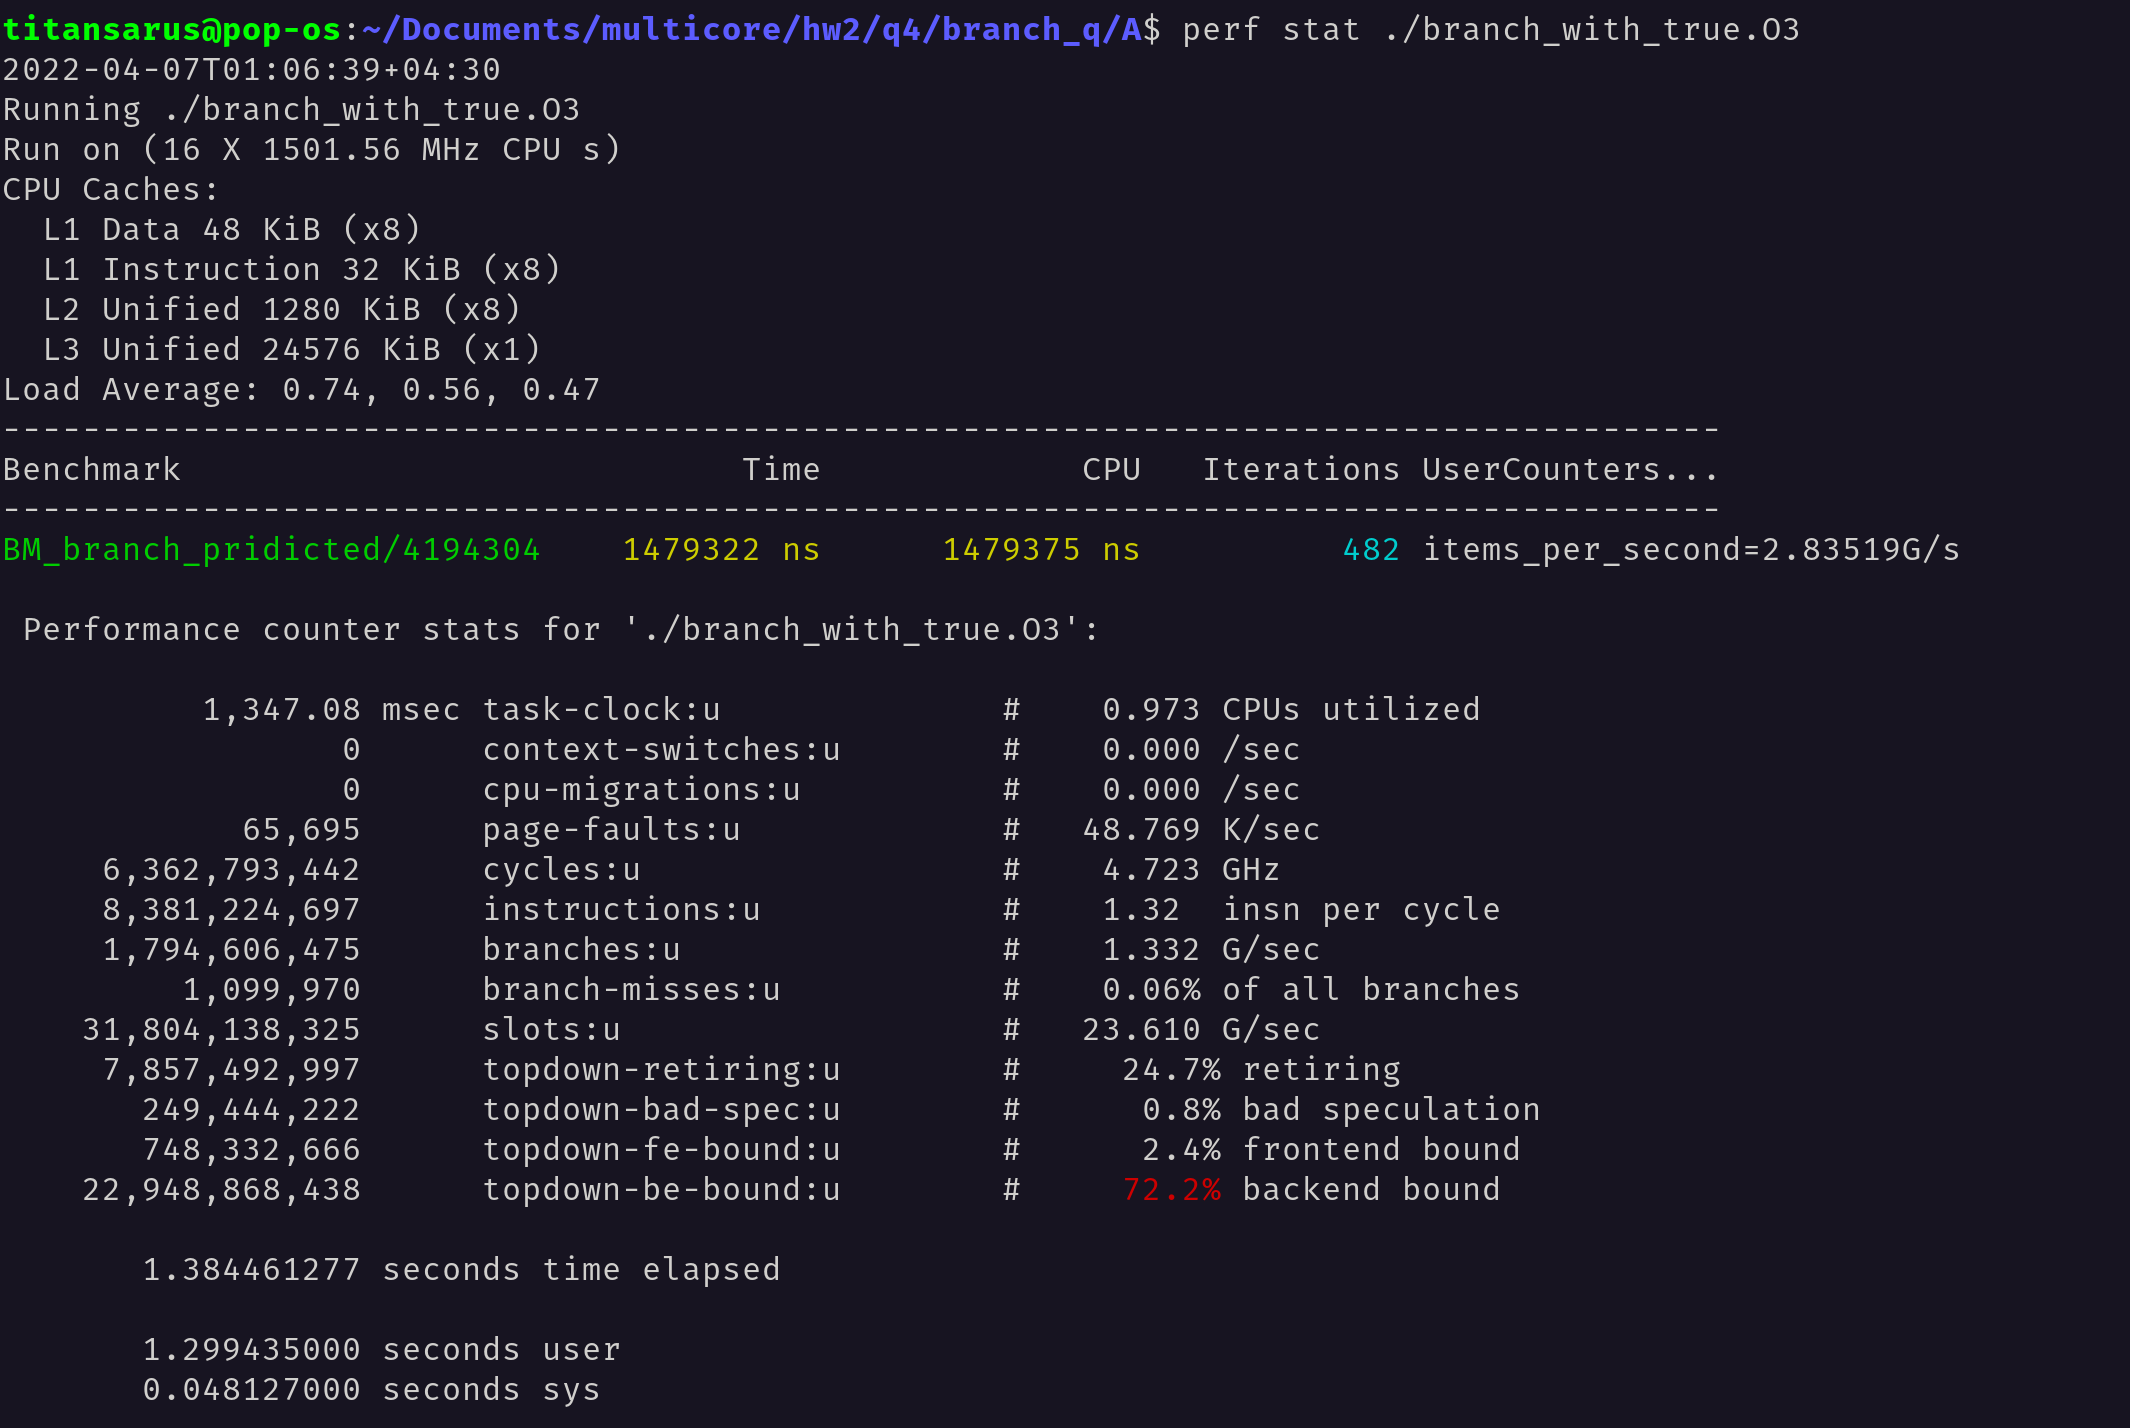
\includegraphics[width=0.8\textwidth]{./images/4A/branch-with-true-o3.png}	
	\cprotect\caption{\Verb+branch_with_true.O3+}
\end{figure}


\begin{figure}[H]
	\centering
	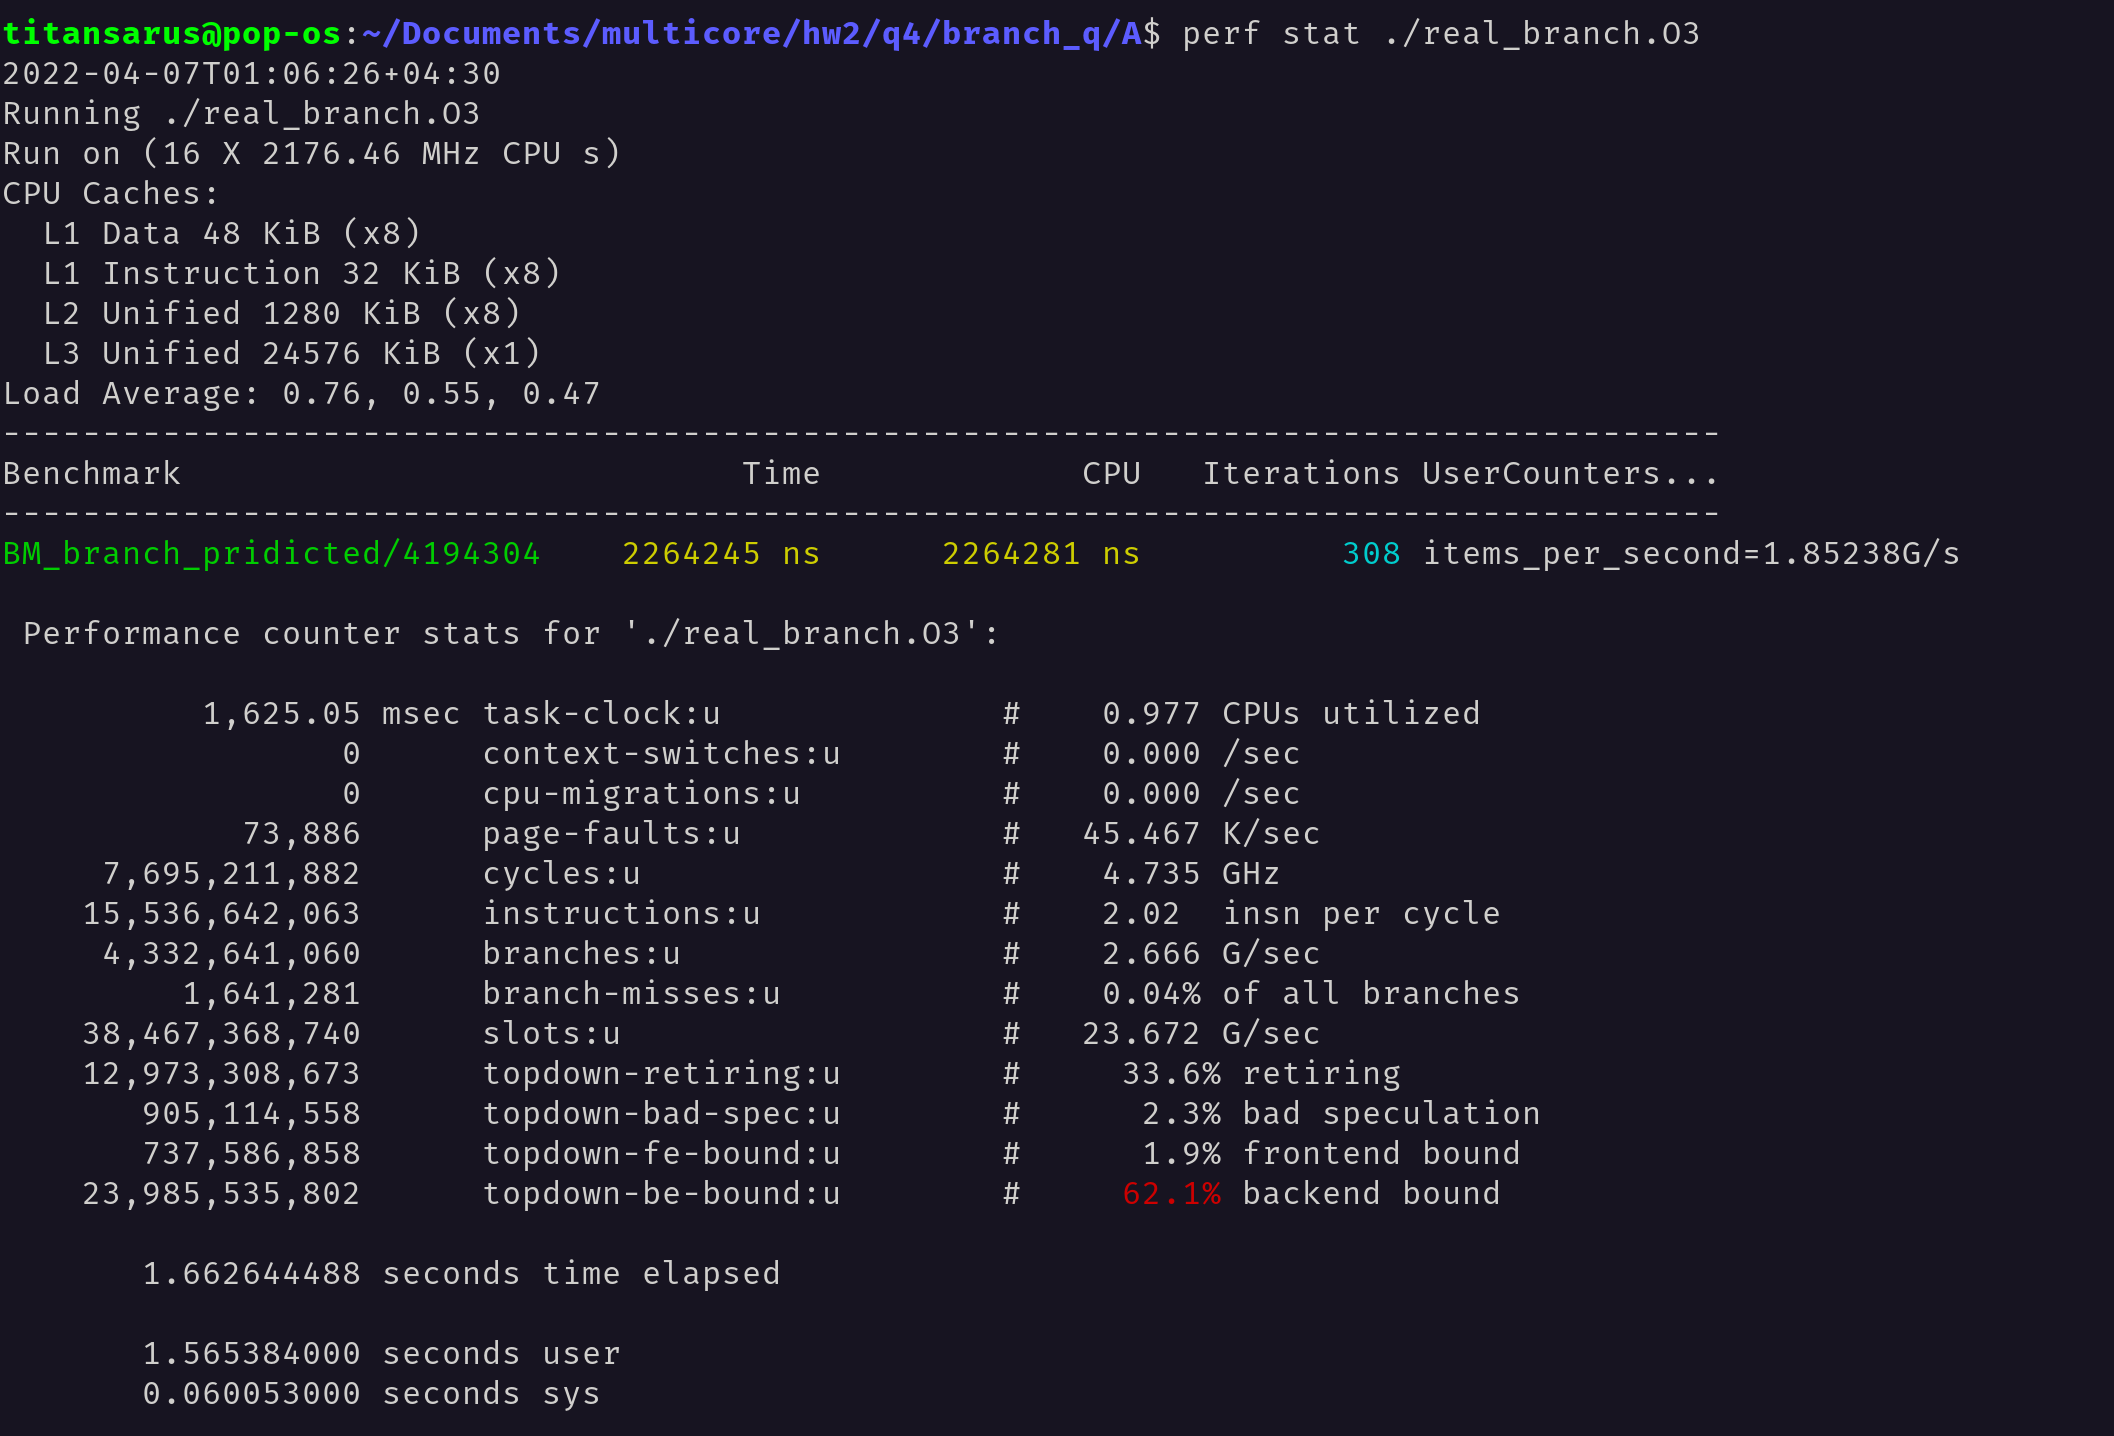
\includegraphics[width=0.8\textwidth]{./images/4A/real-branch-o3.png}	
	\cprotect\caption{\Verb+real_branch.O3+}
\end{figure}

\item
For \Verb+.out+ part, we can see that the fastest is \Verb+no_branch+, then \Verb+real_branch+ and at last \Verb+branch_with_true+.

The reason for \Verb+no_branch+ being the fastest is pretty apparent. It doesn't use any branch in its main logic, while the other two use branches. So it is faster than those two.

The reason for \Verb+real_branch+ being faster than \Verb+branch_with_true+ is a little trickier. Its main reason is that we have a function call in \Verb+branch_with_true+ without optimization. Each function call adds some instructions for stack management and jumps that add to the runtime overhead, while \Verb+real_branch+ only uses memory access to an array on its branch part. These memory accesses can be cached. Due to it being a memory access to contiguous parts of an array, it leverages spatial locality, leading to better performance.


\item 
We can see almost identical results for
\Verb+no_branch.O3+ and \Verb+branch_with_true.O3+. That is because the compiler can see that the branch in \Verb+branch_with_true+ is a call to a function that only returns 1. So it can completely optimize the branch out and use only the true part of \codeword{if}. So the final binary result is almost identical to \Verb+no_branch+ and hence its performance.

\item 
As we can see, we didn't get the same performance boost for \Verb+real_branch.O3+. The reason is that \Verb+real_branch.O3+ uses memory access for its branch condition. This memory elements values come from an expression that has calls to \codeword{rand()} function. Although we know \codeword{rand()} always outputs non-negative numbers, predicting it for the compiler is not easy enough. Therefore it cannot optimize the branch out the way it did with \Verb+branch_with_true.O3+. So we couldn't get the same performance boost.

Even if we replaced \codeword{rand() >= 0} with \codeword{1}, we couldn't still get that performance boost. Because still, the branch depends on an array memory access, and compilers don't optimize memory accesses that aggressively.



	\end{itemize}
	
	
	
	\subsection{B}
	
	\begin{itemize}
		\item 
		Only including important parts of coded needed for explanation:
		
		
\begin{lstlisting}[style=CStyle]
	//branch_0101.cpp
	...
	 c[i] = (i == 0) ? rand() >= 0 : !c[i - 1];
	...
	if (c_ptr[i]) {
		a += p1[i];
	} else {
		a *= p2[i];
	}
	...
\end{lstlisting}
	
		
\begin{lstlisting}[style=CStyle]
	//pure_random.cpp
	...
	c[i] = rand() & 0x1;
	...
	if (c_ptr[i]) {
		a += p1[i];
	} else {
		a *= p2[i];
	}
	...
\end{lstlisting}	

	
		
\begin{lstlisting}[style=CStyle]
	//always_true.cpp
	...
	c[i] =  c[i] = rand() >= 0;
	...
	if (c_ptr[i]) {
		a += p1[i];
	} else {
		a *= p2[i];
	}
	...
\end{lstlisting}	


As we can see, \Verb+always_true+ is almost the same as the last part. \codeword{rand()} always generates a non-negative number, and so the branch condition will always be true.

For \Verb+pure_random+ we have \codeword{c[i] = rand() & 0x1;} which actually means it will be one if the result of \codeword{rand()} is odd, and otherwise it will be zero. Suppose the \codeword{rand()} function is implemented well enough to generate a uniform distribution of random numbers. In that case, it will generate almost equal amounts of zeroes and ones in a uniformly distributed way. So the result of the condition will be purely random.

For \Verb+branch_0101+, we have \codeword{c[i] = (i == 0) ? rand() >= 0 : !c[i - 1];} which causes the result of \codeword{c[i]} to alternate between \codeword{1} and \codeword{0}.

\item
In the following pictures, you can see the output of \Verb+perf stat+ for of all files:

\begin{figure}[H]
	\centering
	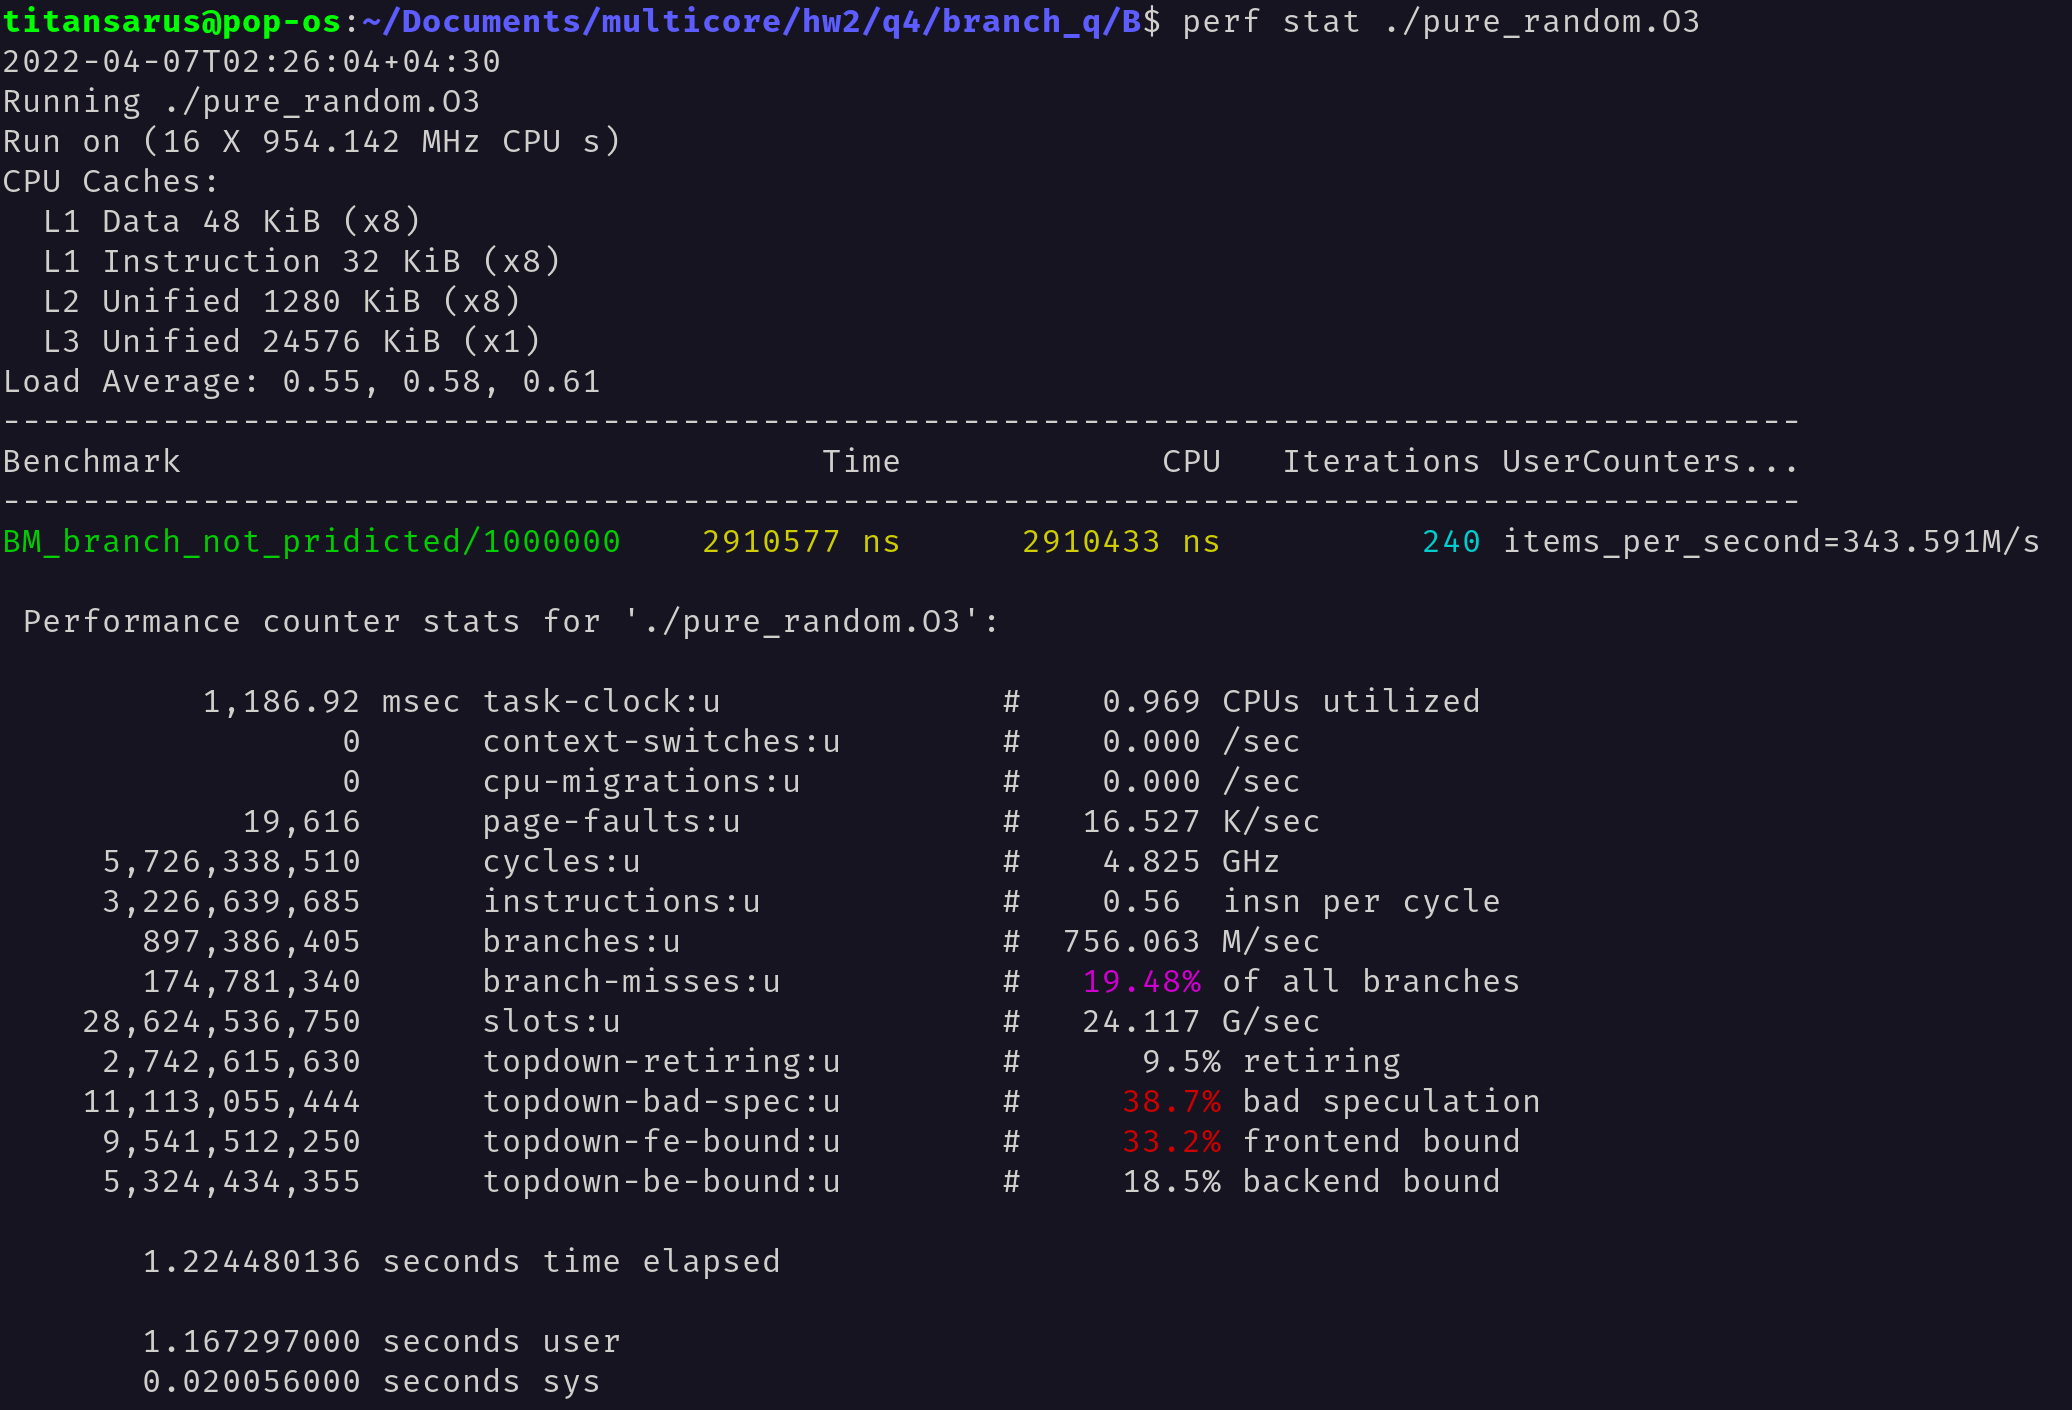
\includegraphics[width=0.75\textwidth]{./images/4B/pure-random.png}	
	\cprotect\caption{\Verb+pure_random.O3+}
\end{figure}



\begin{figure}[H]
	\centering
	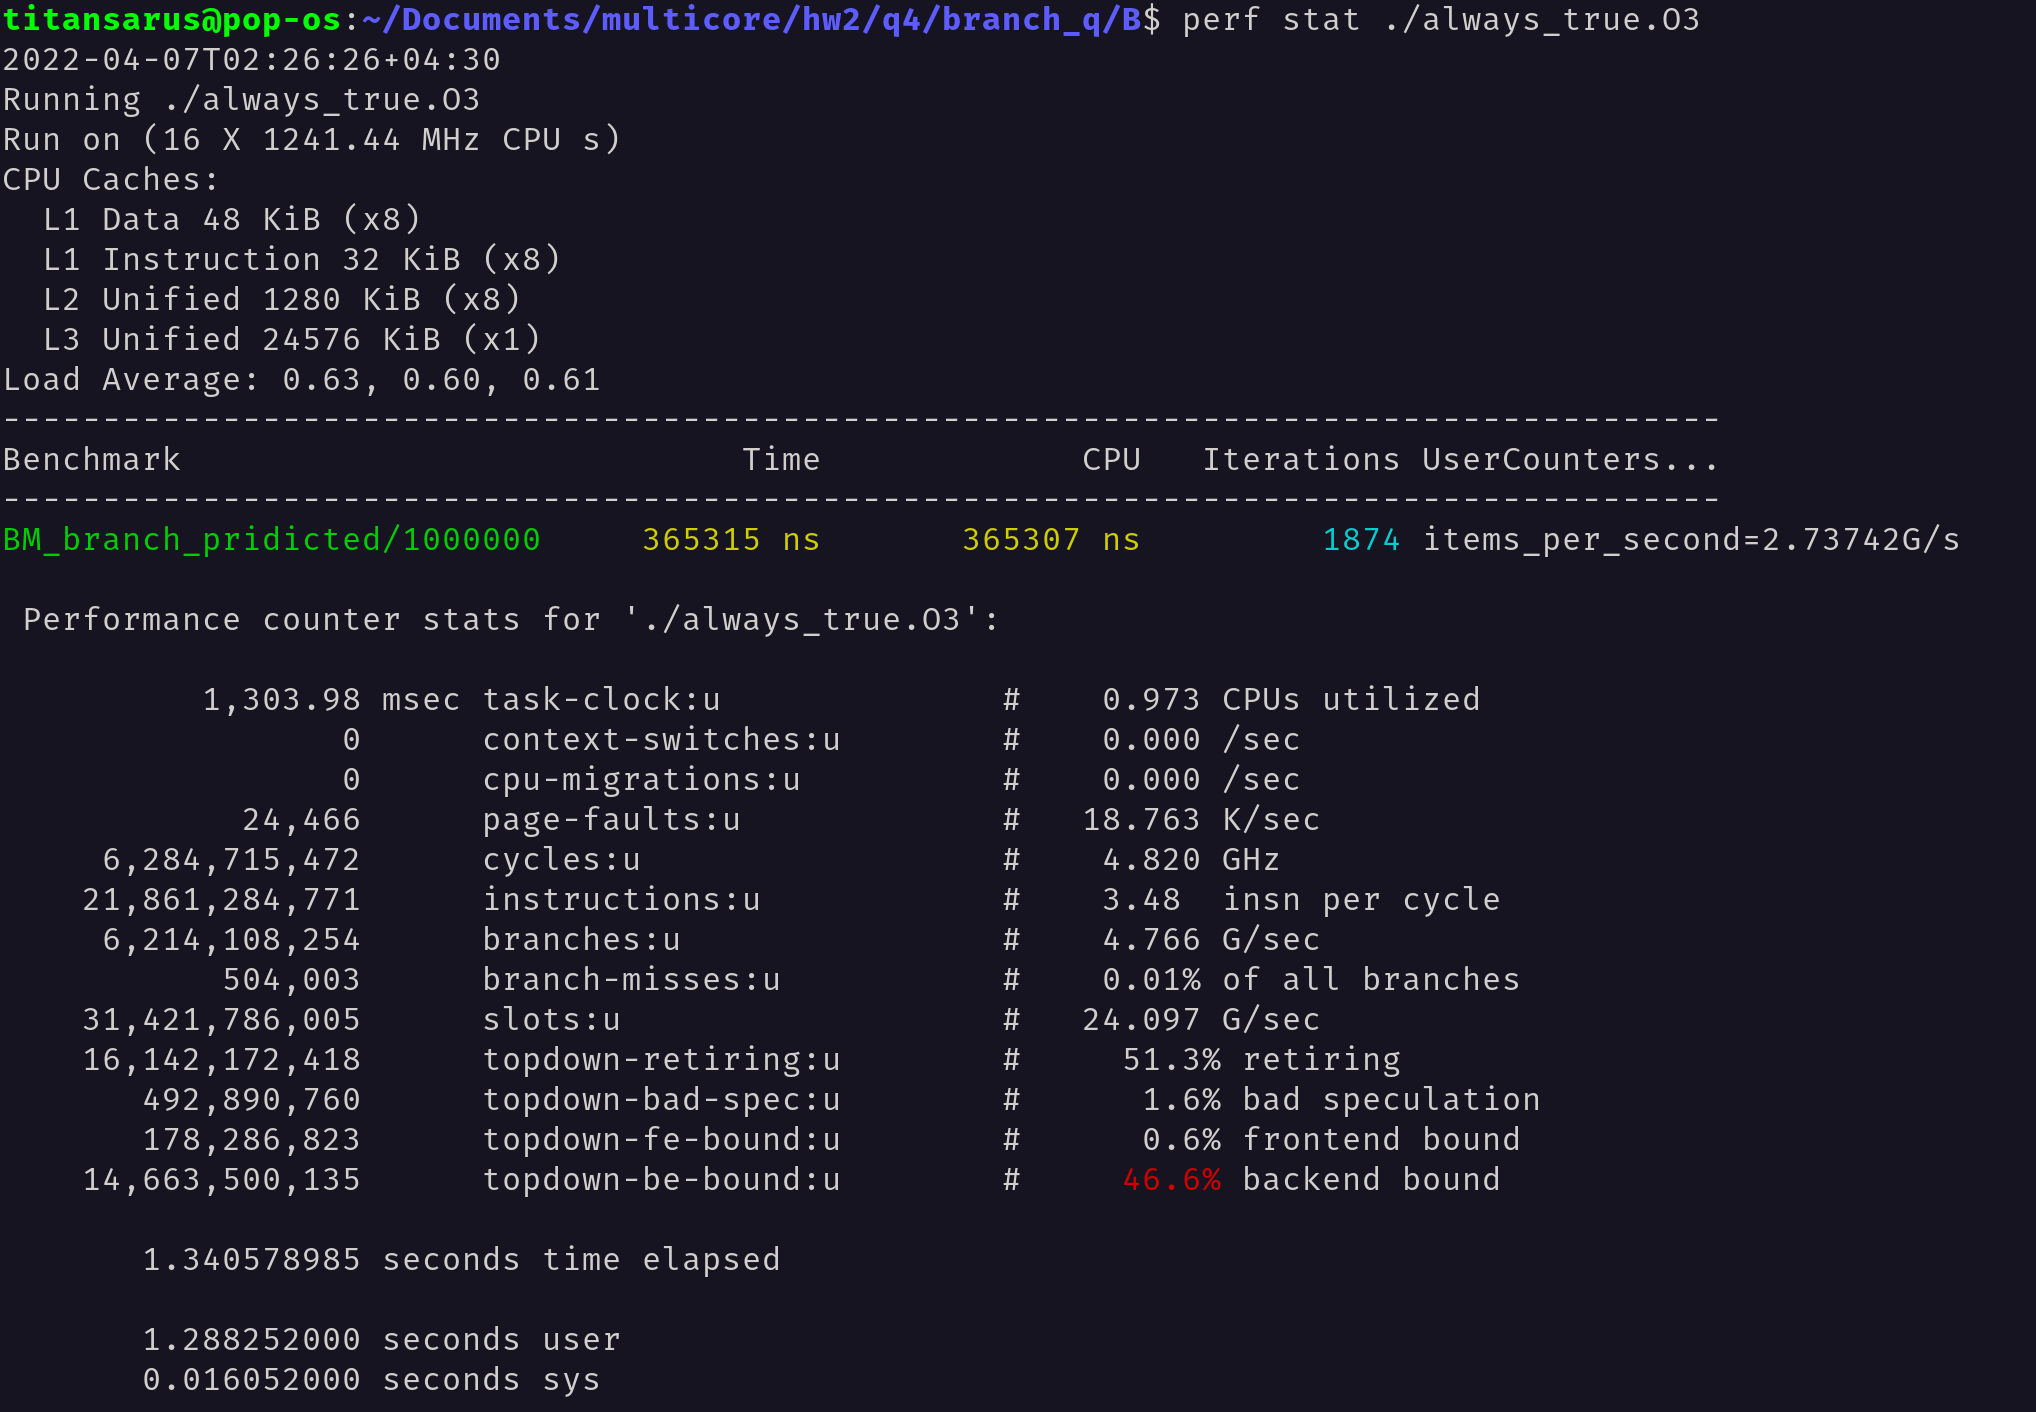
\includegraphics[width=0.75\textwidth]{./images/4B/always-true.png}	
	\cprotect\caption{\Verb+always_true.O3+}
\end{figure}

\begin{figure}[H]
	\centering
	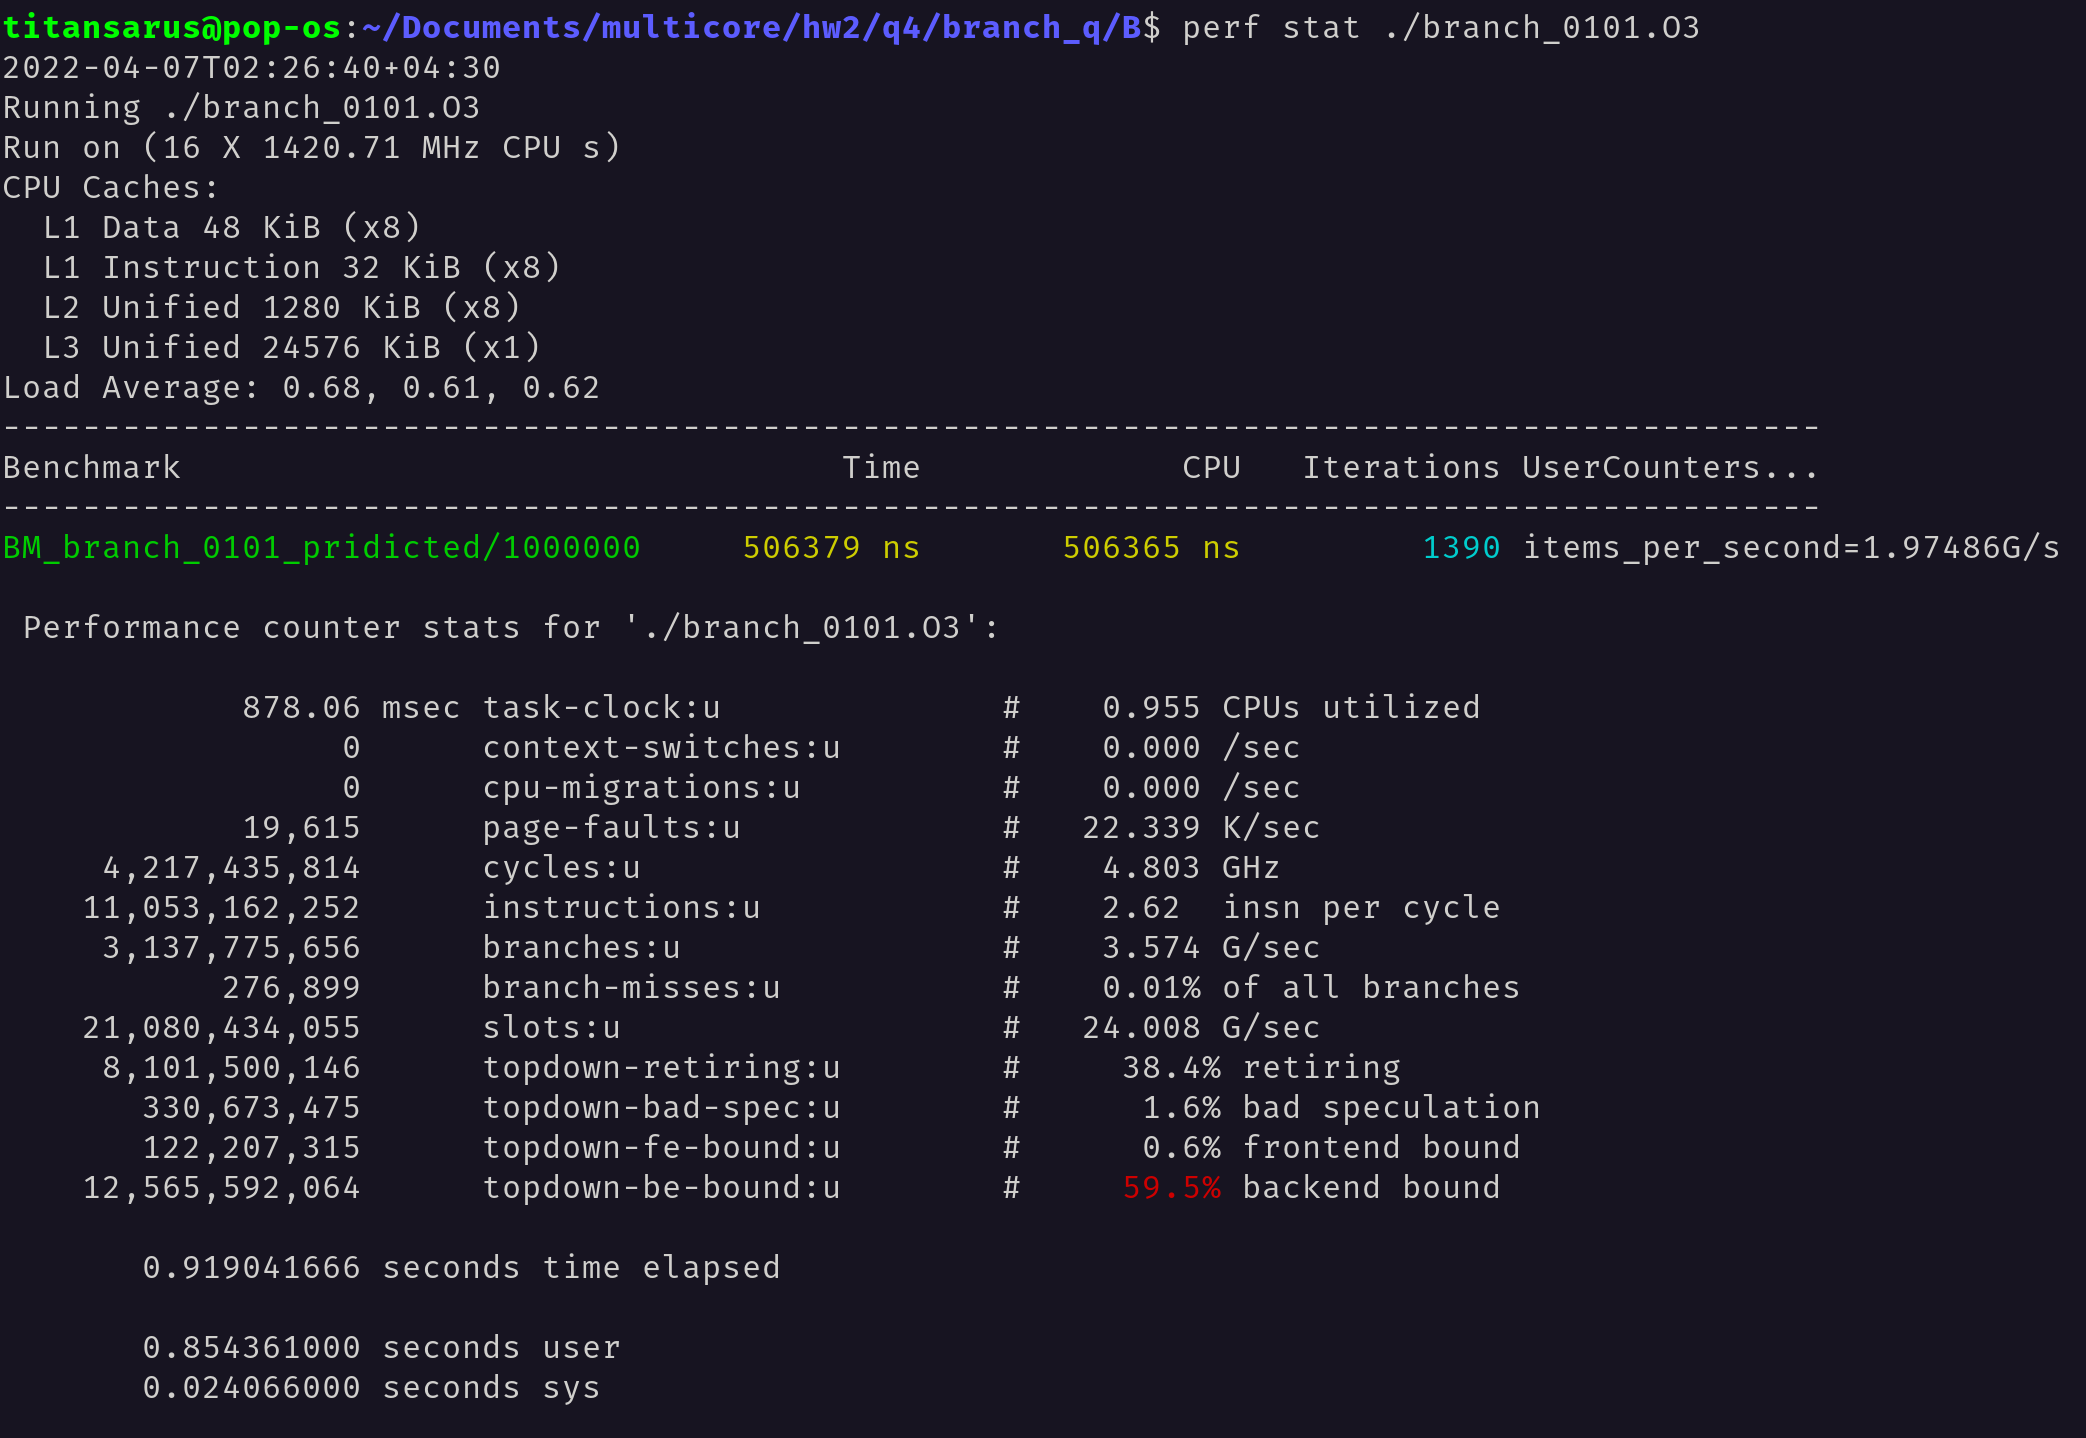
\includegraphics[width=0.75\textwidth]{./images/4B/branch-0101.png}	
	\cprotect\caption{\Verb+branch_0101+}
\end{figure}

\item 
In the \Verb+always_true+ we can see a tiny percentage for branch-miss ratio. The CPU's branch predictor easily finds out the branch constantly evaluates to true, and therefore, its speculative execution always prefers the true part of the condition.

In the \Verb+pure_random+, the pattern for branch condition being true or false is purely random, and therefore, most of the time, the CPU cannot predict it well enough; therefore, we see a substantial branch-miss ratio of about $20\%$.

\item 
A lot can be said about the tolerable branch-miss ratio. By just investigating the result of \Verb+perf+ in this problem, it seems miss-ratio in the order of $1\%$ or less is tolerable, but if we get into the $15\%-20\%$ range, it will be not as tolerable.

We investigated this case further. Looking at the textbook, we can see some charts about the branch-miss ratio.

\begin{figure}[H]
	\centering
	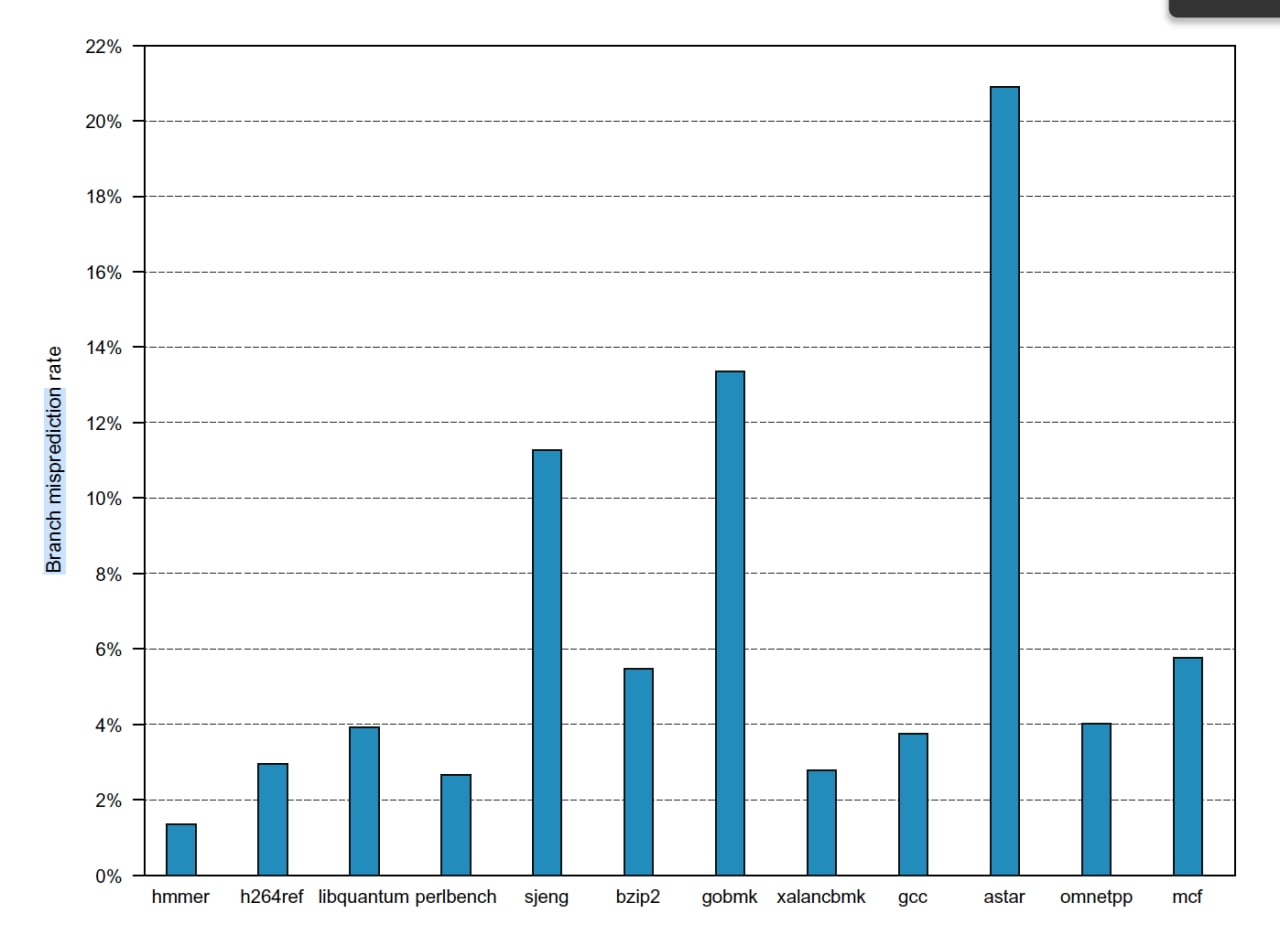
\includegraphics[width=0.6\textwidth]{./images/branchmiss1.jpg}
	\caption{}	
	\label{fig:branch1}
\end{figure}

\begin{figure}[H]
	\centering
	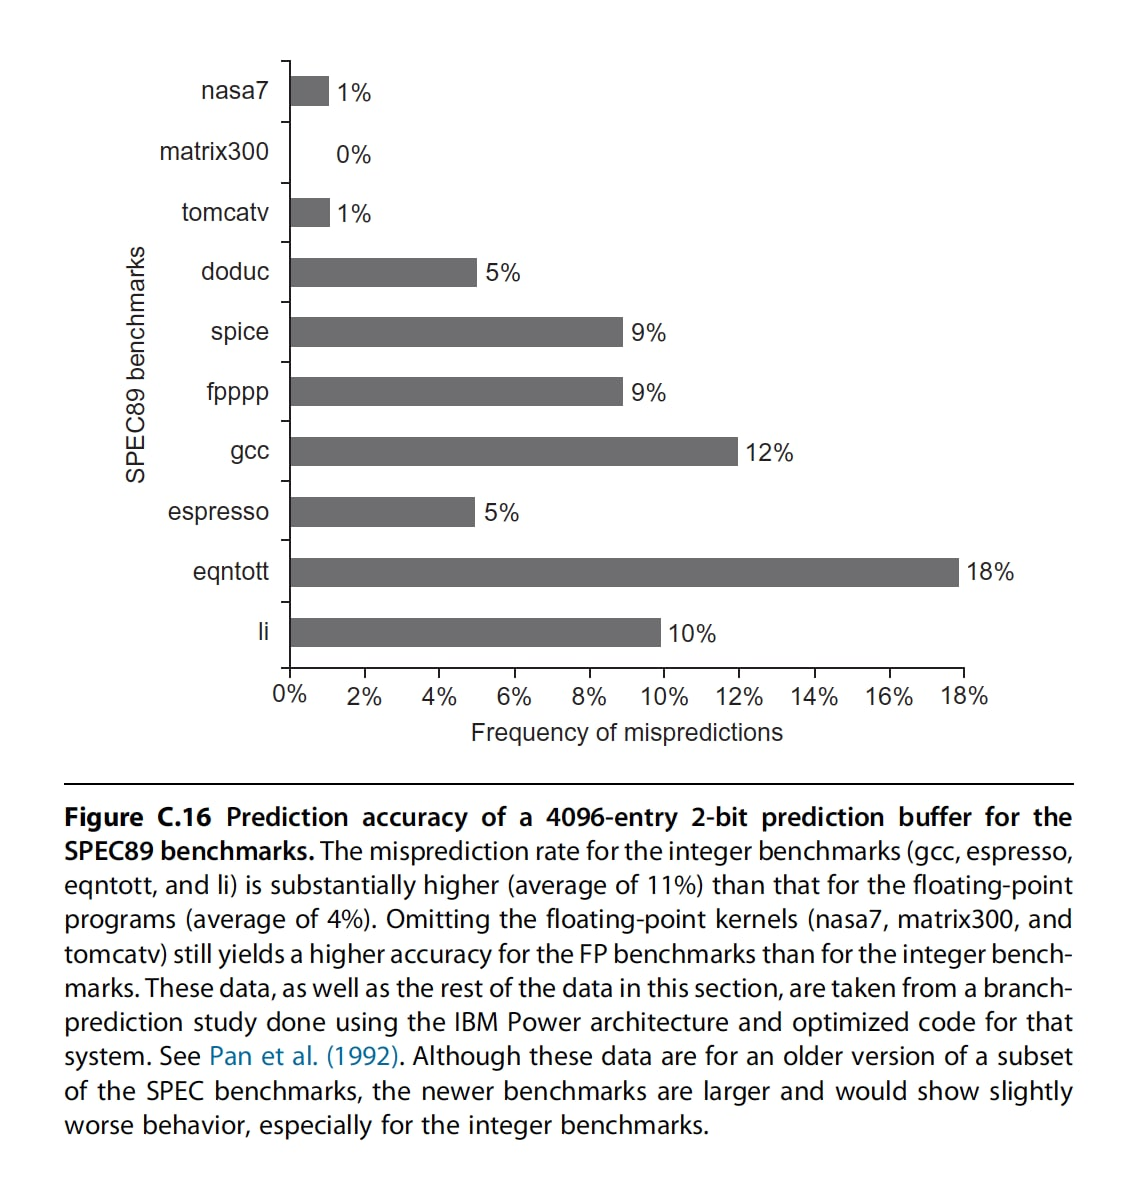
\includegraphics[width=0.6\textwidth]{./images/branchmiss2.jpg}
	\caption{}	
	\label{fig:branch2}
\end{figure}

The figure \ref{fig:branch1} specifies miss-ratio for some programs included in SPEC benchmark. As we can see, in most cases, the miss-ratio is in the order of $5\%$. So it seems that $5\%$ is a tolerable ratio. The only exceptions in this chart are \Verb+sjeng+,\Verb+gobmk+ and \Verb+astar+. The high branch-miss ratio for these comes from their stochastic nature. \Verb+astar+ runs $A^*$ algorithm on some randomly generated maps. \Verb+gobmk+ is an artificial intelligence program for the Go game, and \Verb+sjeng+ is an artificial intelligence program for chess. As the state space of these programs can explode exponentially, and some parts of their algorithms rely on random and stochastic processes, we see a huge miss-ratio.

Figure \ref{fig:branch2} shows accuracy of a 4096-entry 2-bit prediction buffer for SPEC89. For this part, We quote a paragraph from the book about the misprediction rate:

\begin{quote}
	What kind of accuracy can be expected from a branch-prediction buffer using 2
	bits per entry on real applications? Figure C.16 shows that for the SPEC89 benchmarks
	a branch-prediction buffer with 4096 entries results in a prediction accuracy ranging from over 99\% to 82\%, or a misprediction rate of 1\%–18\%. A 4K entry
	buffer, like that used for these results, is considered small in 2017, and a larger
	buffer could produce somewhat better results.
\end{quote}

\item 

$$\text{branch-miss-per-iteration}_\text{branch-0101}=\frac{276899}{1390}=199.21$$

$$\text{branch-miss-per-iteration}_\text{always-true}=\frac{504003}{1874}=286.95$$

It seems odd that branch-miss for \Verb+always_true+ is higher than \Verb+branch_0101+. It is because the CPU had run so many iterations that the branch misses of \Verb+becnhmark+ library affected the results. As we can see, the overall iteration count of \Verb+always_true+ is also higher. Still, as \Verb+perf stat+ runs independently of the code and counts branch misses of \Verb+benchmark+ library, the overhead of running so many iterations caused \Verb+always_true+ to have more branch-miss per iteration.

\item 
As we can see, the branch-miss ratio of \Verb+branch_0101+ and \Verb+always_true+ are comparable, but \Verb+pure_random+ has a much higher branch-miss ratio. This is because the CPU's branch predictor uses some history tables and can easily recognize the $1010101010$ pattern that is occurring in the \Verb+branch_0101+ and also, it can always recognize true patterns even more efficiently. But it obviously cannot predict a purely random pattern, and this causes lots of branch misses.

	\end{itemize}
	
	
	
	
	\subsection{C}
	\begin{itemize}
			\item 
	Only including important parts of coded needed for explanation:
	
	\begin{lstlisting}[style=CStyle]
		//always_true.cpp
		...
		c[i] =  c[i] = rand() >= 0;
		...
		if (c_ptr[i]) {
			a += p1[i];
		} else {
			a *= p2[i];
		}
		...
	\end{lstlisting}

	\begin{lstlisting}[style=CStyle]
	//also_always_true.cpp
	...
 	c1[i] = rand() & 0x1;
	c2[i] = !c1[i];
	...
	if (c1_ptr[i] || c2_ptr[i]) {
		a += p1[i];
	} else {
		a *= p2[i];
	}
	...
\end{lstlisting}

\Verb+always_true+ is the same as previous cases. For the \Verb+also_always_true+ we can see that \codeword{c2[i]} is always negate of \codeword{c1[i]} and as we know $p \lor \neg p \equiv 1$, so the \codeword{if} condition of this case will also always evaluate to true.

\item 

In the following pictures, you can see the output of \Verb+perf stat+ for of all files:

\begin{figure}[H]
	\centering
	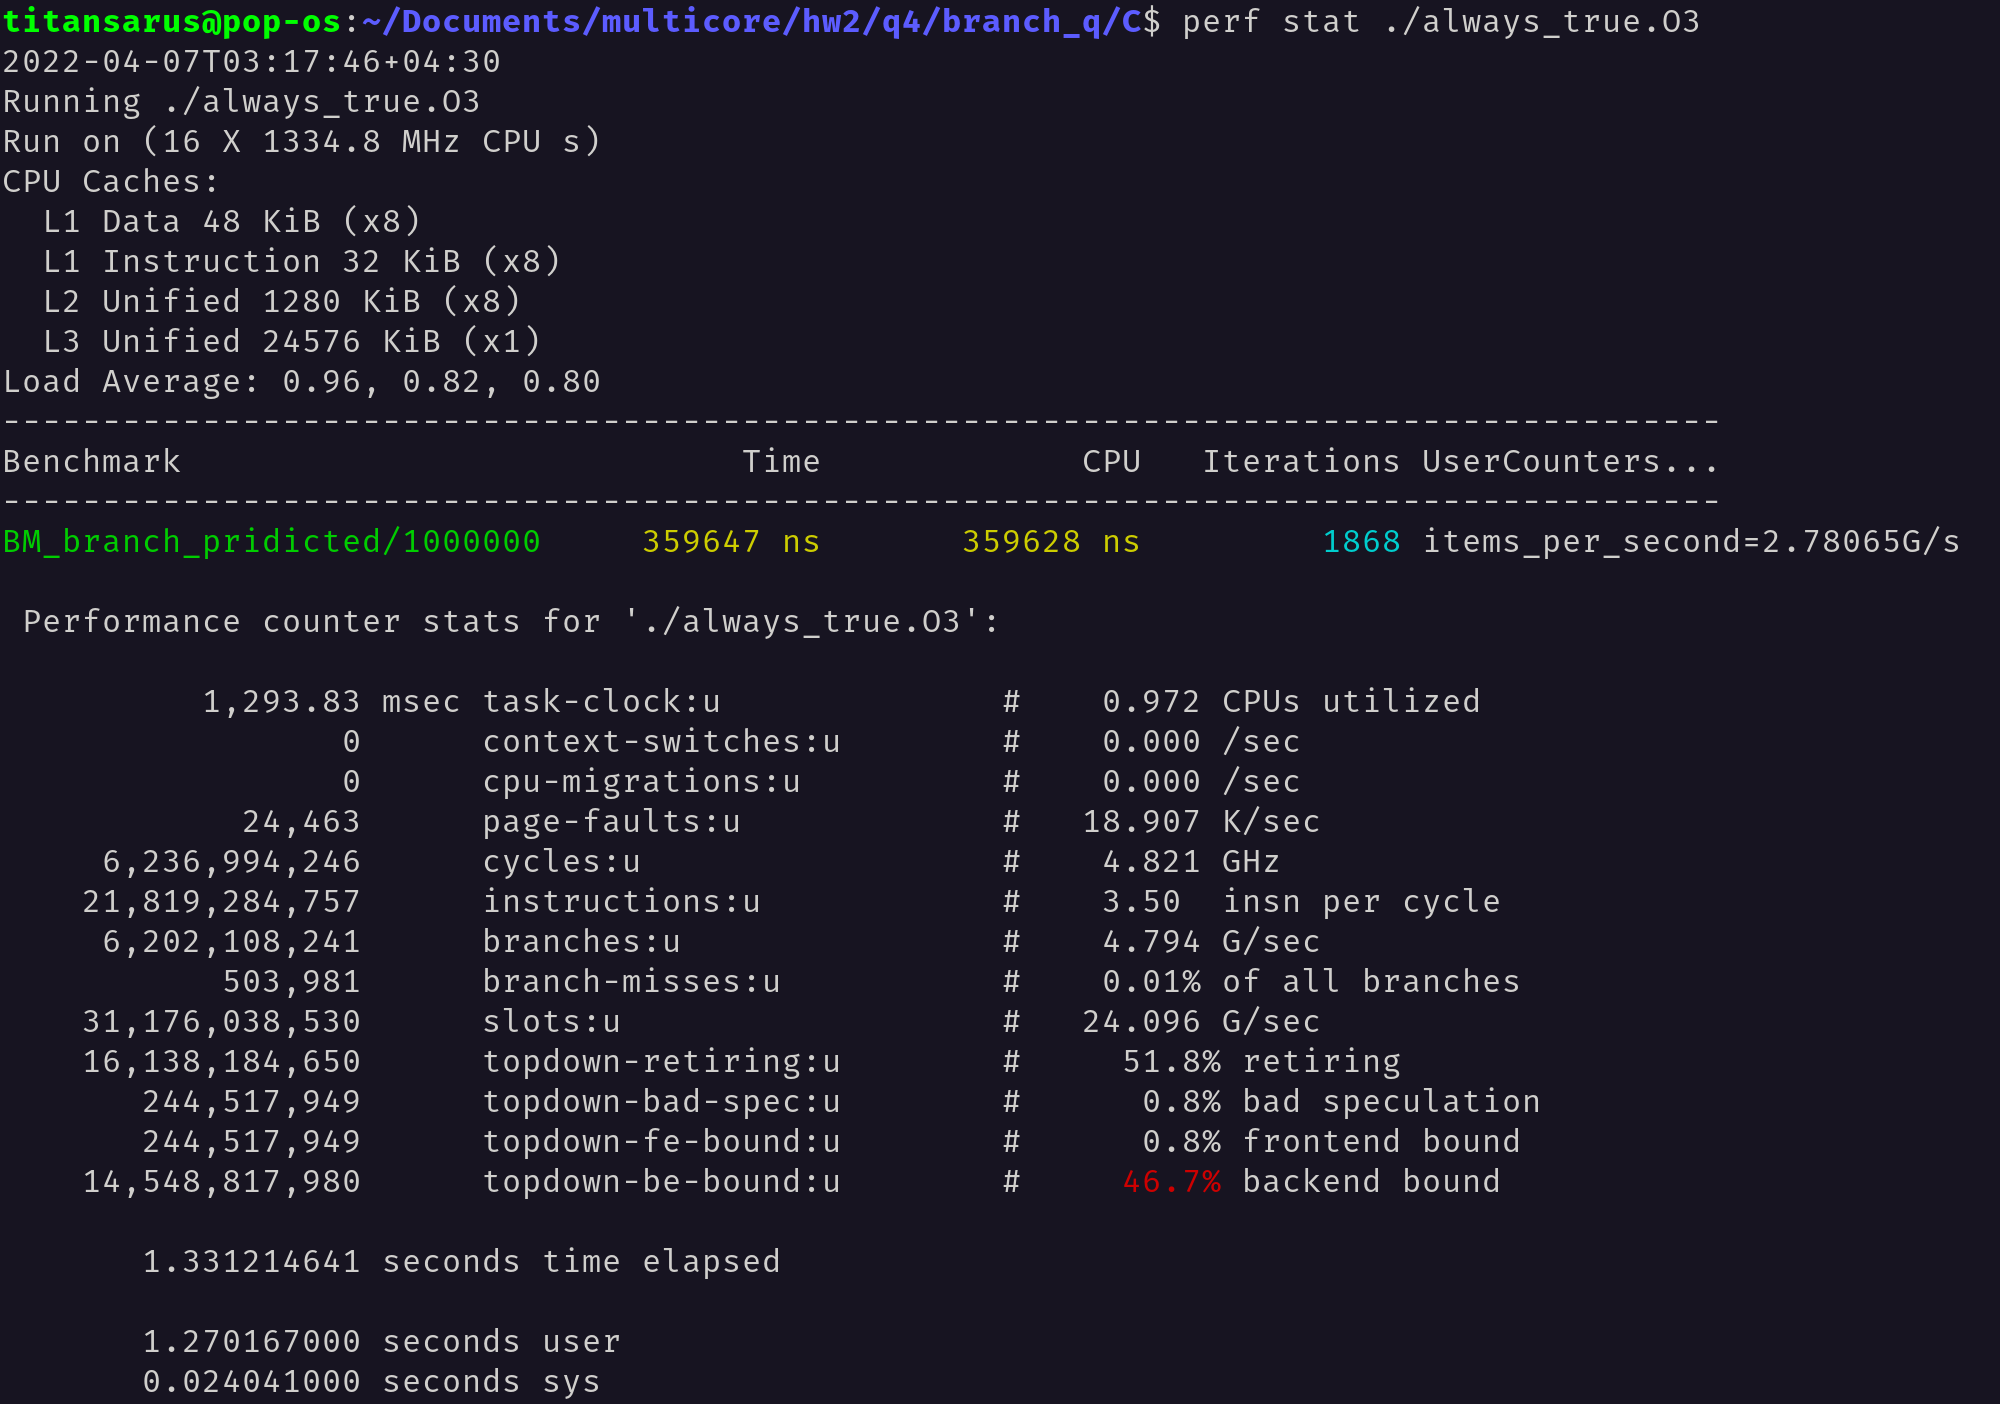
\includegraphics[width=0.75\textwidth]{./images/4C/always-true.png}	
	\cprotect\caption{\Verb+always_true.O3+}
\end{figure}


\begin{figure}[H]
	\centering
	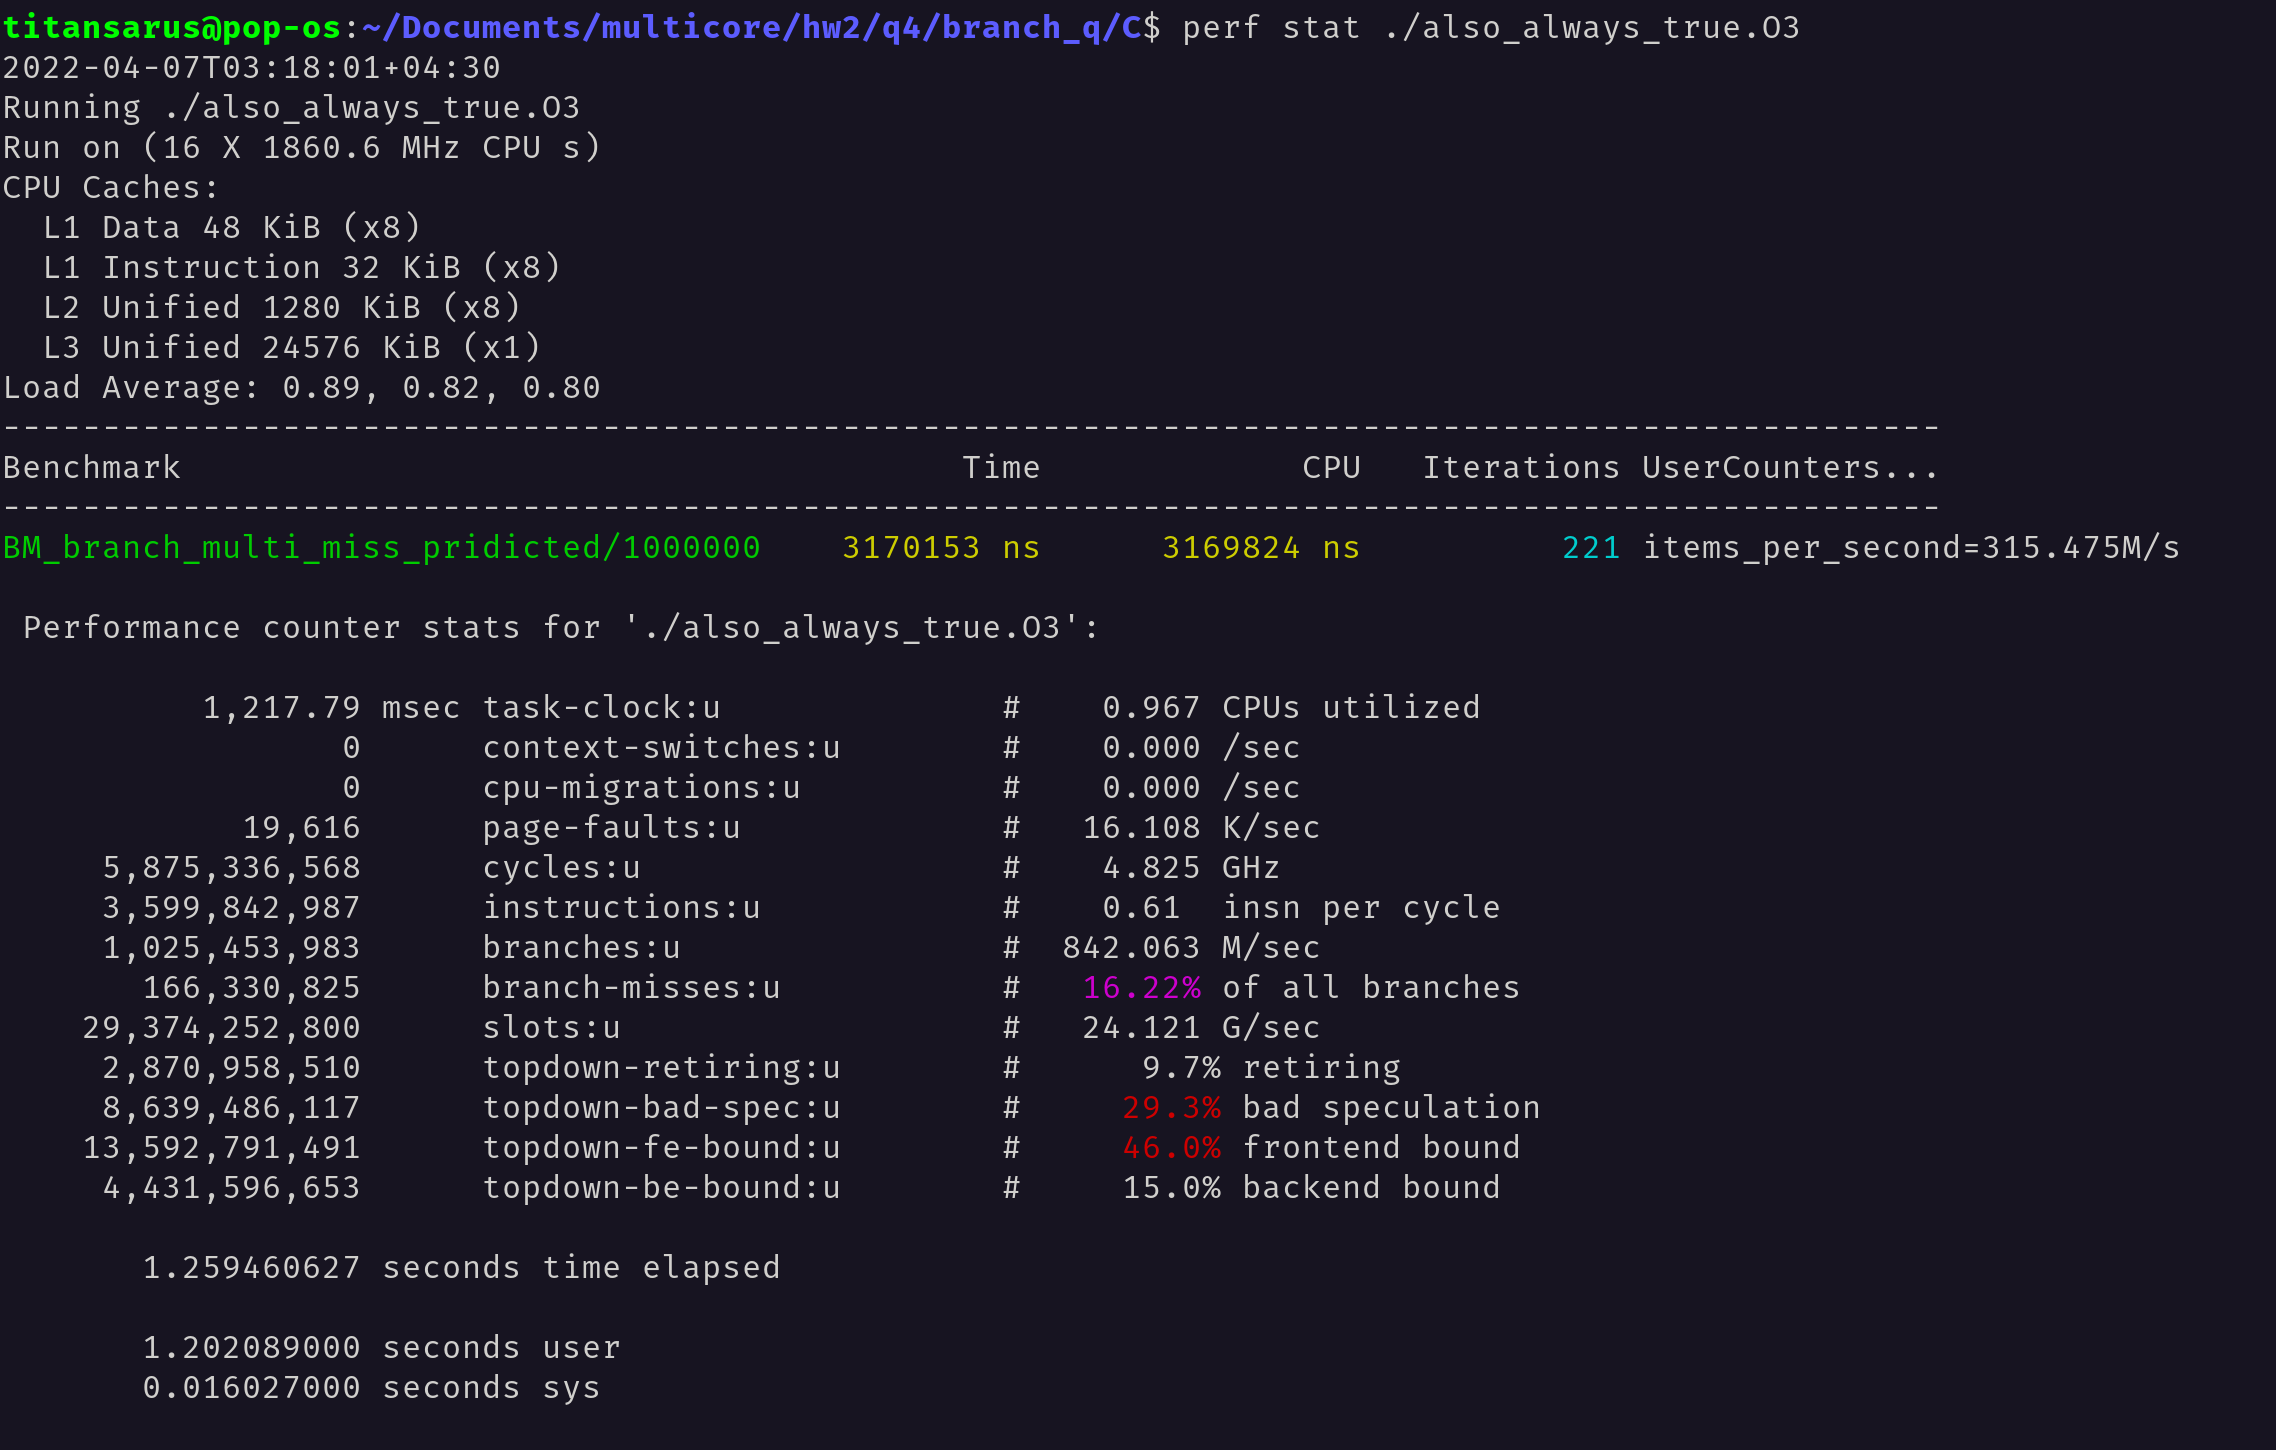
\includegraphics[width=0.75\textwidth]{./images/4C/also-always-true.png}	
	\cprotect\caption{\Verb+also_always_true.O3+}
\end{figure}


\begin{figure}[H]
	\centering
	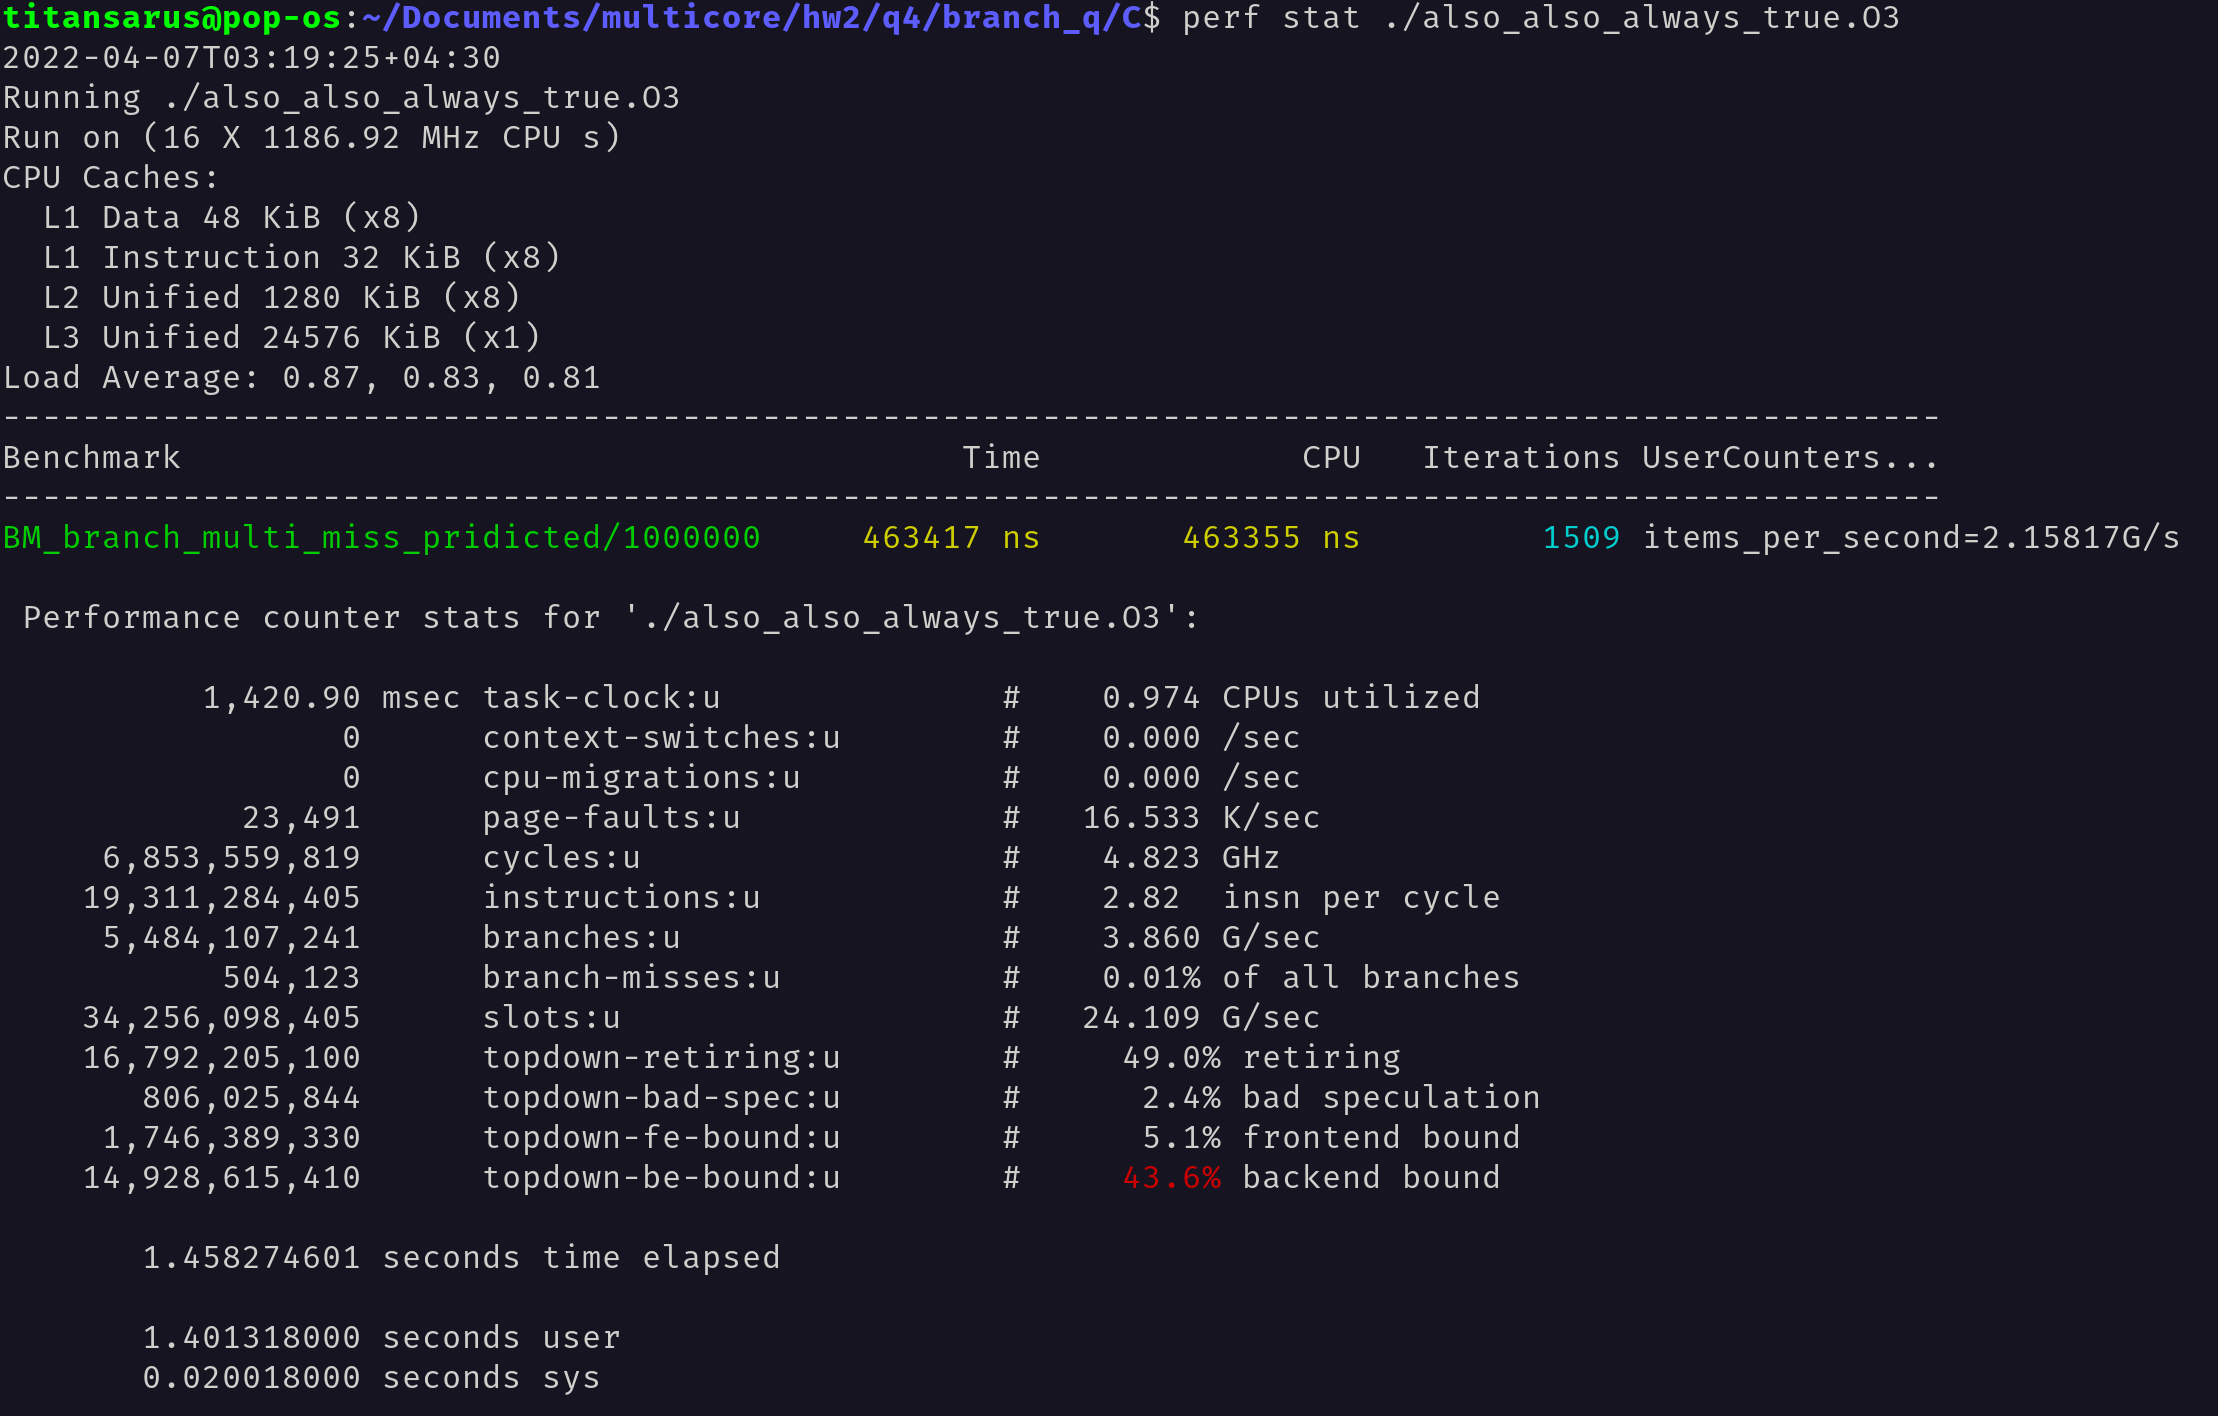
\includegraphics[width=0.75\textwidth]{./images/4C/also-also-always-true.png}	
	\cprotect\caption{\Verb+also_also_always_true.O3+. We generated this new case by replacing \codeword{||} with \codeword{|}}
\end{figure}


\item
As we see, \Verb+also_always_true+ has a huge miss ratio despite the fact that the actual branch condition is always evaluated to true. It is because of the \codeword{||} operator in C. This operator can cause short circuits, i.e., if the first operand is true, the second operand will not be evaluated. To implement this type of functionality compiler is actually generating two branches. In other words,

\begin{lstlisting}[style=CStyle]
	if (condition1 || condition2)
	{
		// do something
	}
\end{lstlisting}

is equal to

\begin{lstlisting}[style=CStyle]
	if (condition1)
	{
		// do something
	} else {
		if (condition2)
		{
			// do something
		}
	}
\end{lstlisting}

Generating two branches to implement short-circuit functionality causes the CPU's branch predictor to miss a lot of branches. Despite the result of the overall or condition being true, if we see each condition as separate branches, they will follow an almost random pattern like what we saw in previous parts, so the CPU's branch predictor will not perform well enough.

If we replace \codeword{||} and \codeword{|}, we get rid of short-circuit functionality and force the program to evaluate the whole expression and see this as a single branch. In this case, it will perform like \verb+always_true+. Because the CPU branch predictor can easily recognize the always true pattern of this branch and it will perform well.


\end{itemize}

	
	\subsection{D}
	\begin{itemize}
	\item 
	
	Important parts of branchless Codes:
	
	
	\begin{lstlisting}[style=CStyle]
		//single_branch_branchless
		
		            a += p1[i] * (c_ptr[i] != 0);
		//            if (c_ptr[i])
		//                a += p1[i];
	\end{lstlisting}
	
	
		\begin{lstlisting}[style=CStyle]
		//pure_random_branchless
		
    bool flag= c_ptr[i]!=0;
		a = (a+ p1[i] * (flag)) * (p2[i] * (!flag) + 1 * (flag));
	//            if (c_ptr[i]) {
	//                a += p1[i];
	//            } else {
	//                a *= p2[i];
	//            }
	\end{lstlisting}
	


	
\begin{lstlisting}[style=CStyle]
	//also_always_true_branchless
	
  bool flag= c1_ptr[i] | c2_ptr[i];
	a = (a+ p1[i] * (flag)) * (p2[i] * (!flag) + 1 * (flag));
	//            if (c1_ptr[i] || c2_ptr[i]) {
	//                a += p1[i];
	//            } else {
	//                a *= p2[i];
	//            }
\end{lstlisting}

Note the usage of \codeword{|} instead of \codeword{||} in \Verb+also_always_true_branchless+. It is because \codeword{||} will be implemented as a branch by the compiler to have the short-circuit functionality, but \codeword{|} doesn't have this functionality and therefore will be a simple bitwise or.

\item 
In the following pictures, you can see the output of \Verb+perf stat+ for of all files:

\begin{figure}[H]
	\centering
	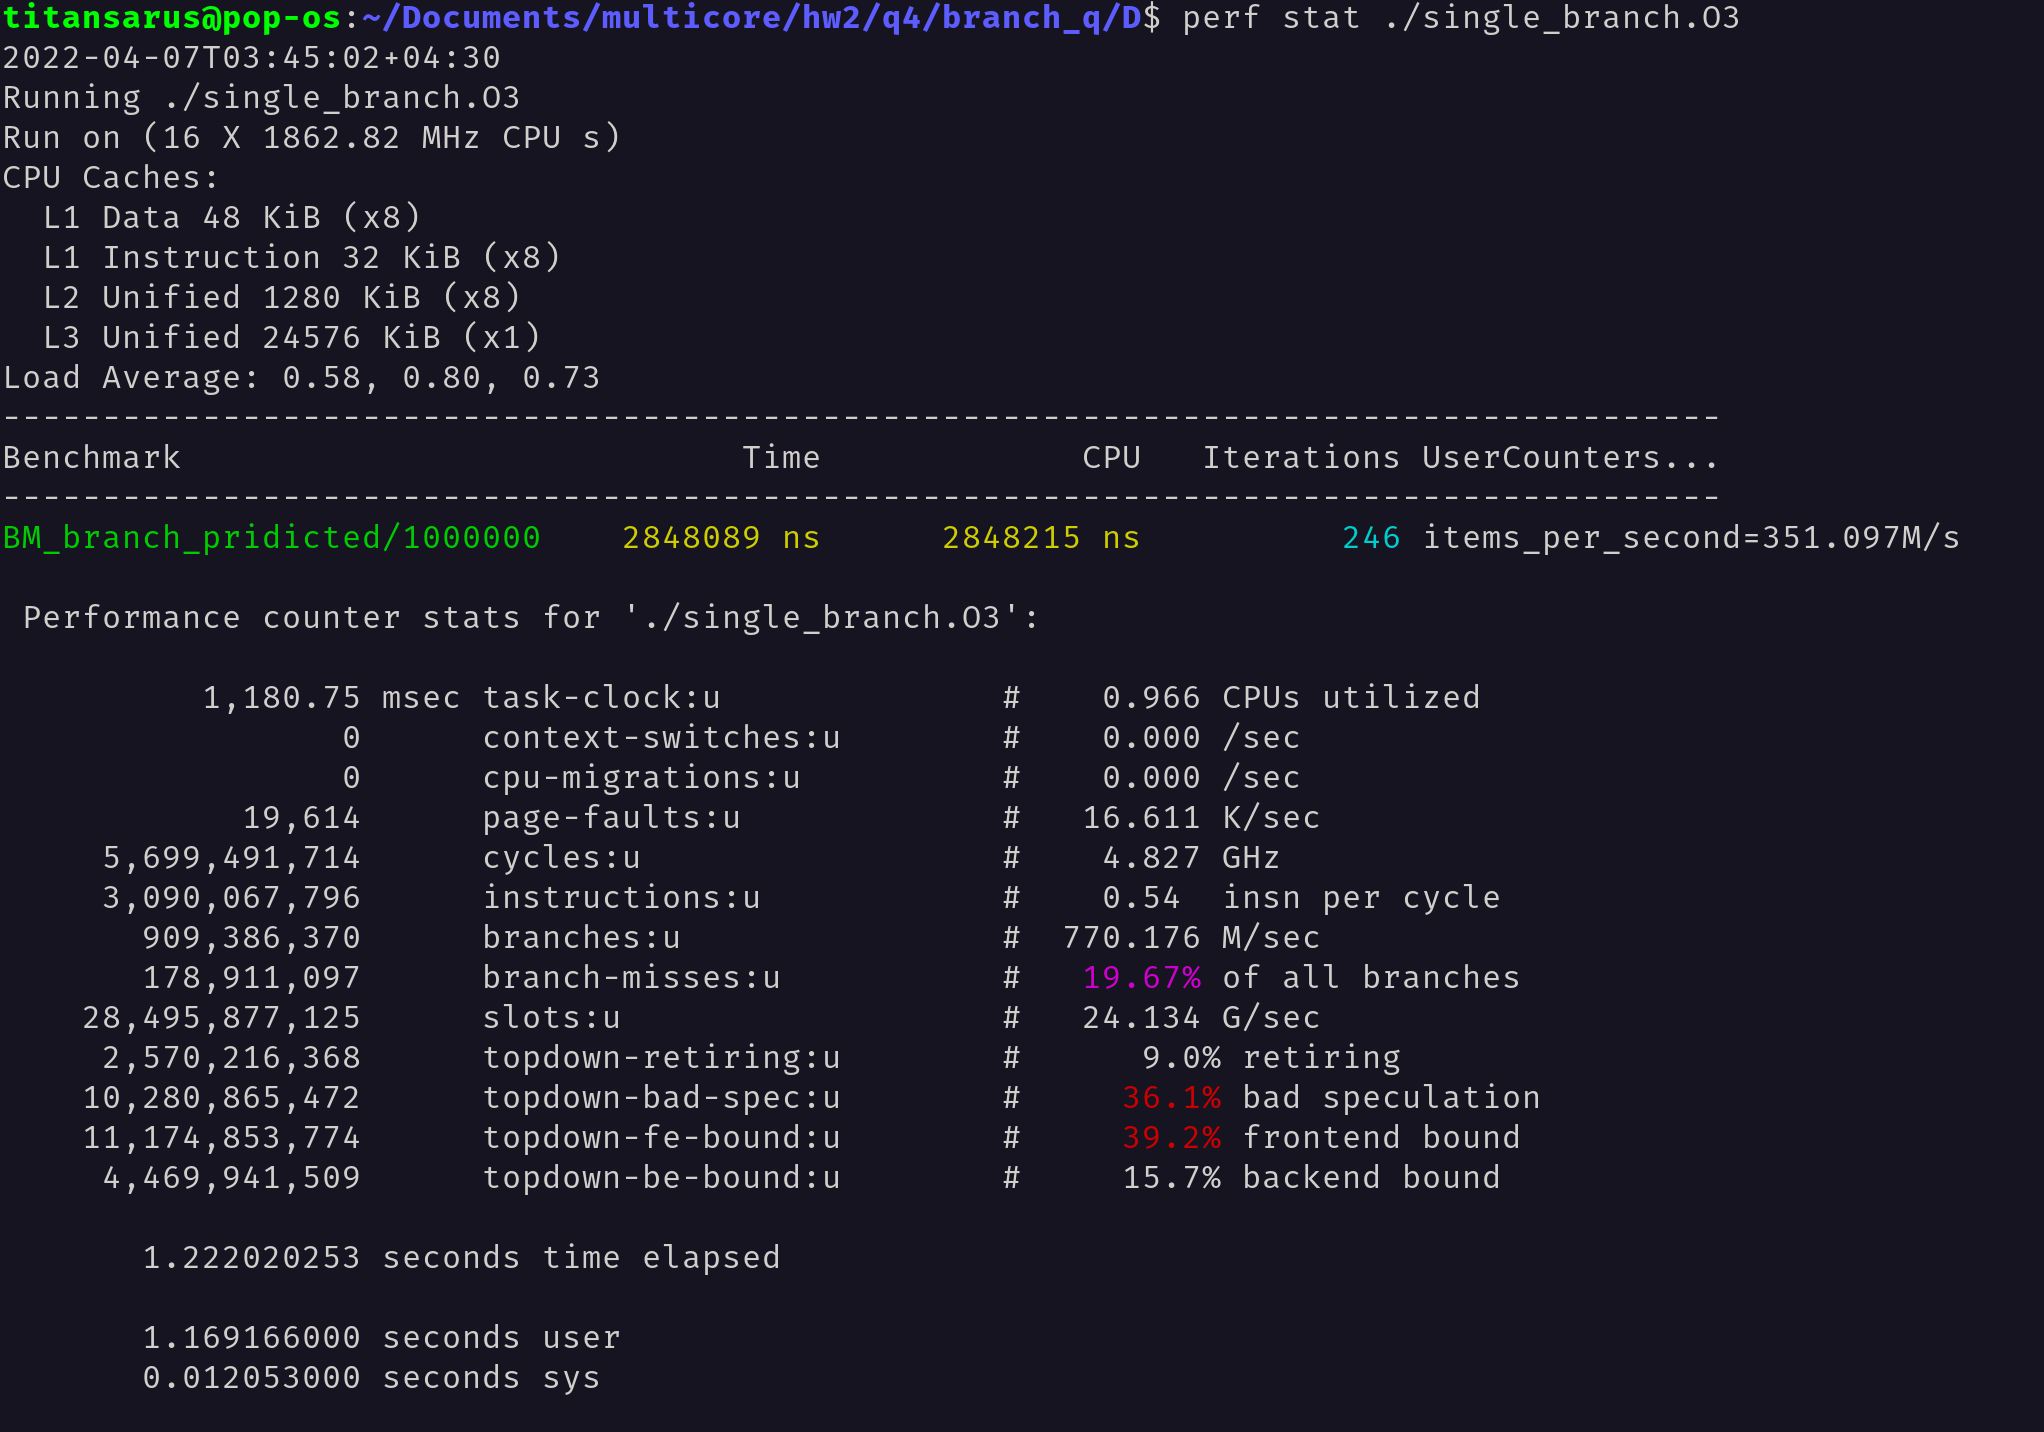
\includegraphics[width=0.75\textwidth]{./images/4D/single-branch.png}	
	\cprotect\caption{\Verb+single_branch.O3+}
\end{figure}


\begin{figure}[H]
	\centering
	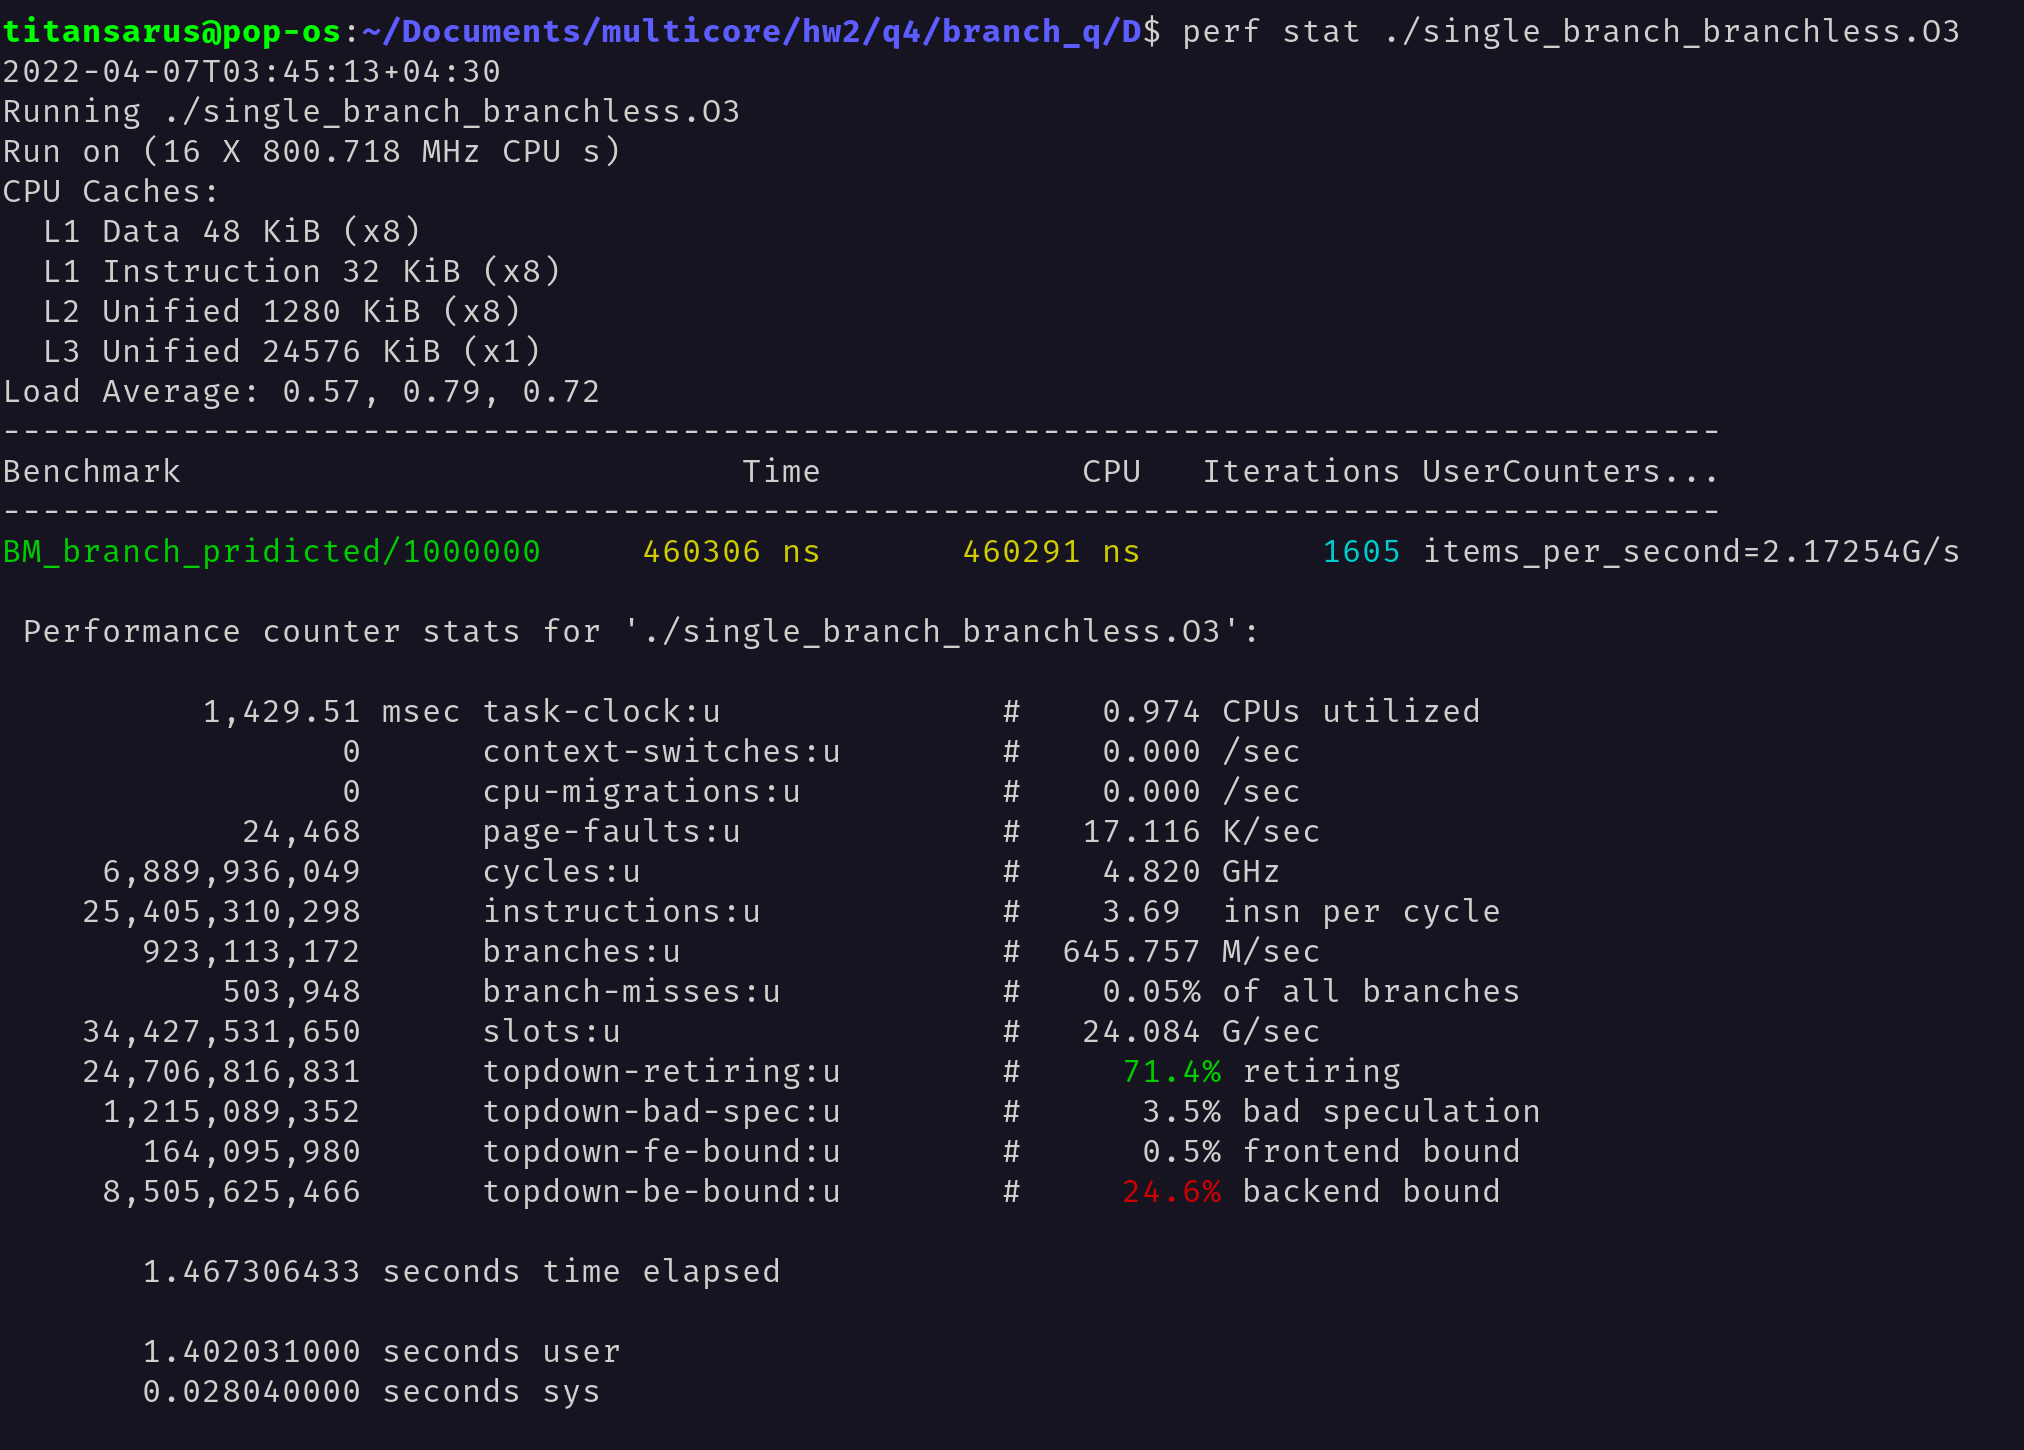
\includegraphics[width=0.75\textwidth]{./images/4D/single-branch-b.png}	
	\cprotect\caption{\Verb+single_branch_branchless.O3+}
\end{figure}


\begin{figure}[H]
	\centering
	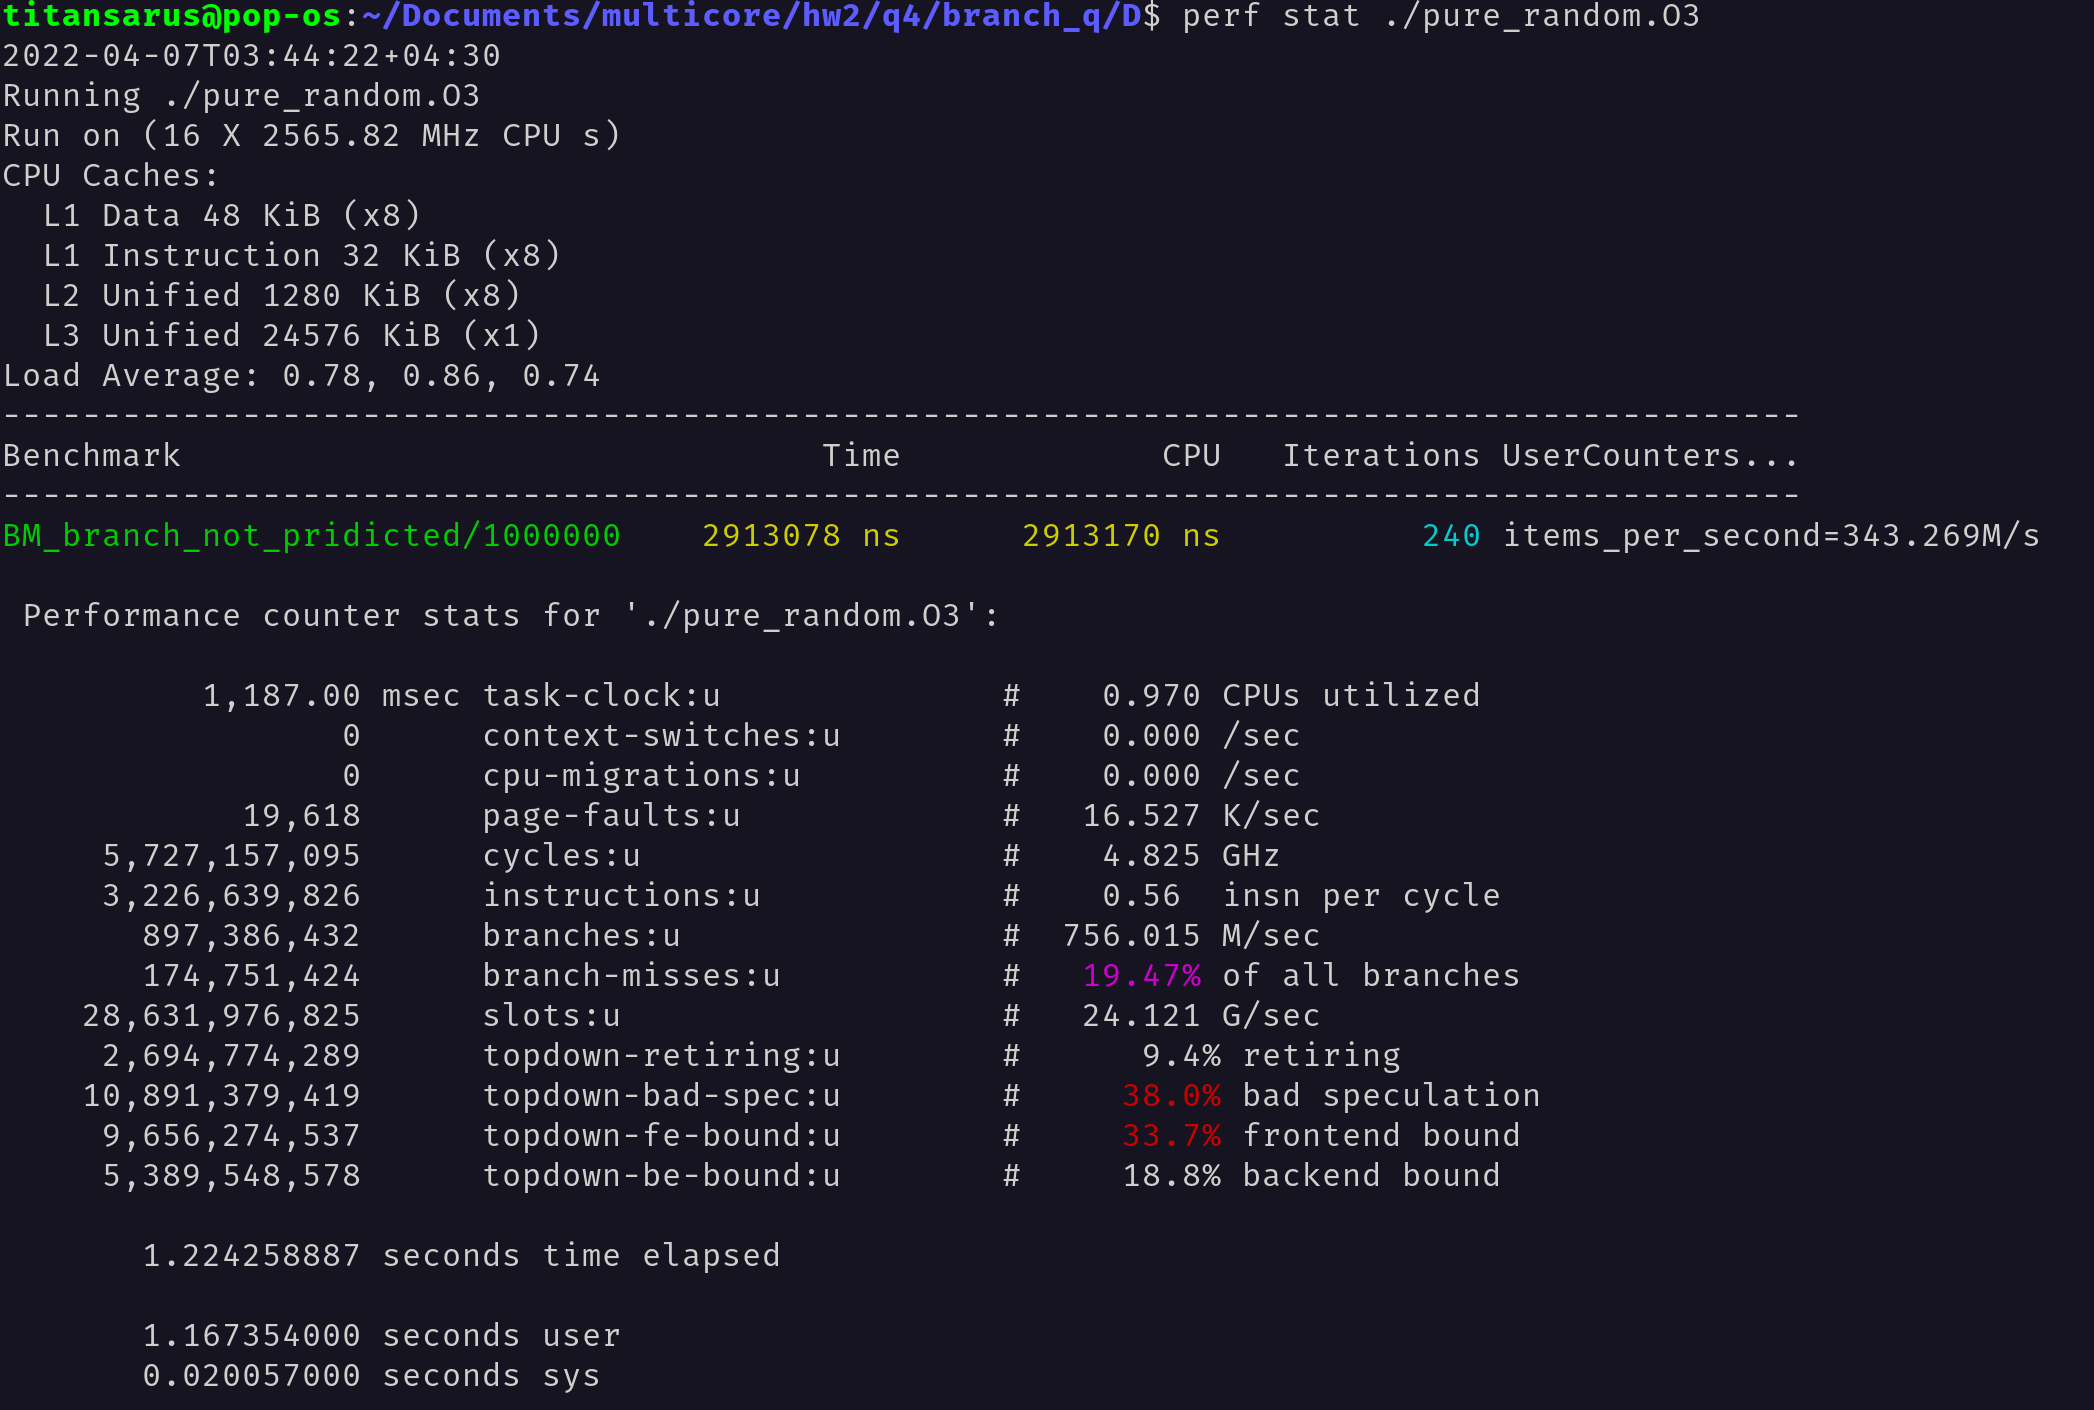
\includegraphics[width=0.75\textwidth]{./images/4D/pure-random.png}	
	\cprotect\caption{\Verb+pure_random.O3+}
\end{figure}


\begin{figure}[H]
	\centering
	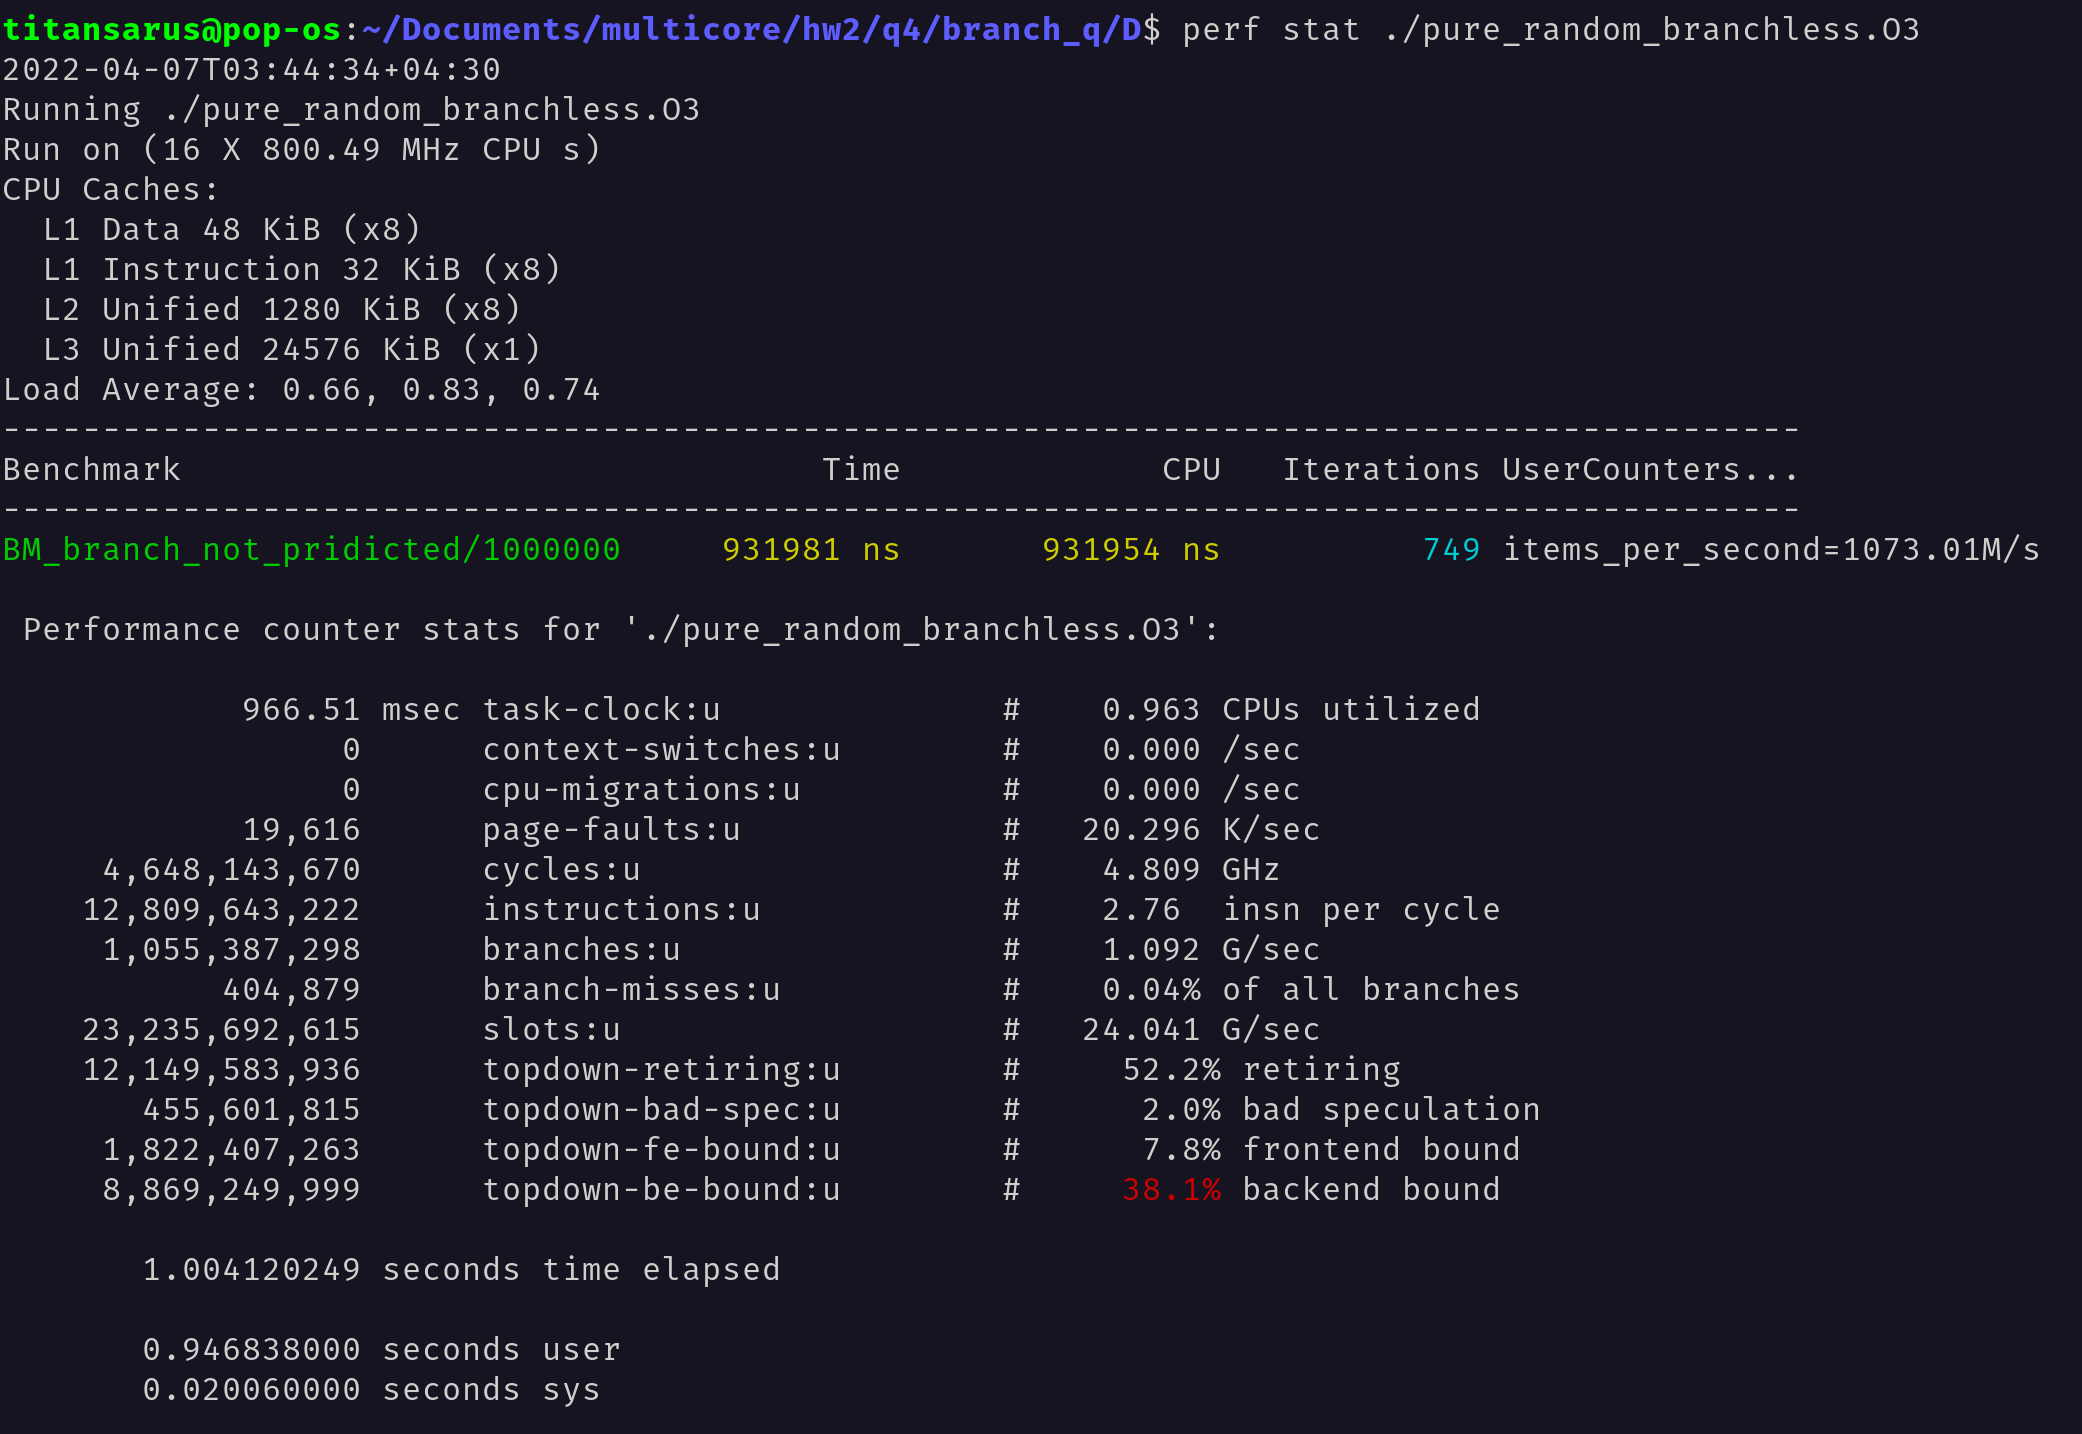
\includegraphics[width=0.75\textwidth]{./images/4D/pure-random-b.png}	
	\cprotect\caption{\Verb+pure_random_branchless.O3+}
\end{figure}


\begin{figure}[H]
	\centering
	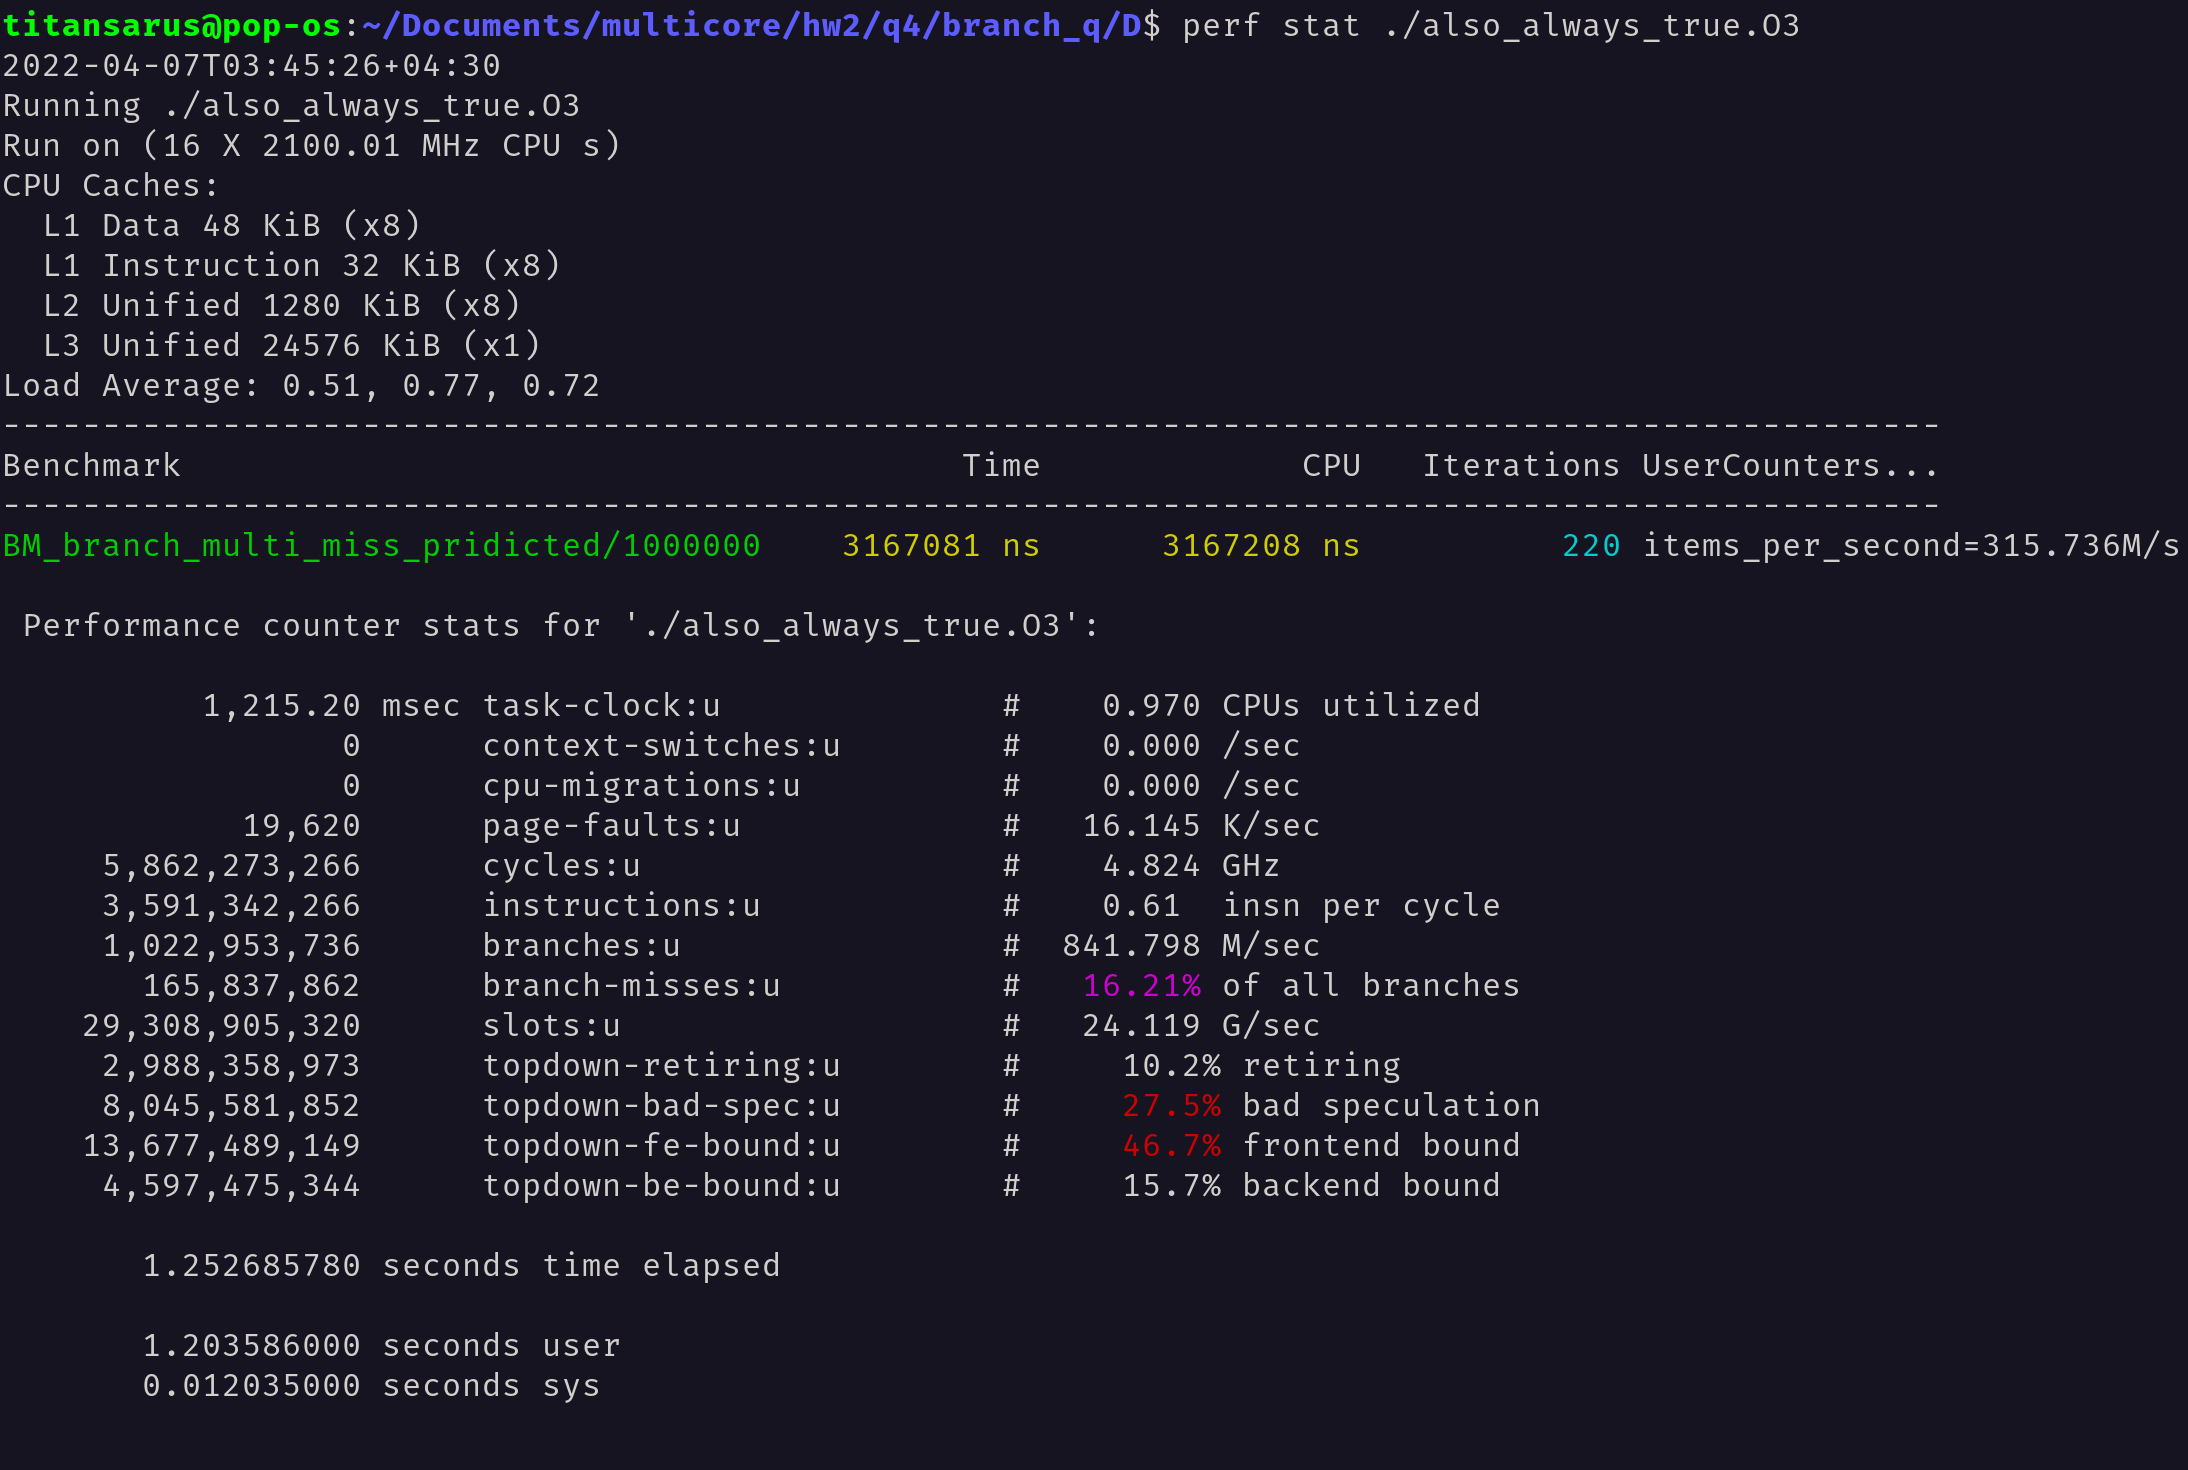
\includegraphics[width=0.75\textwidth]{./images/4D/also-always-true.png}	
	\cprotect\caption{\Verb+also_always_true.O3+}
\end{figure}


\begin{figure}[H]
	\centering
	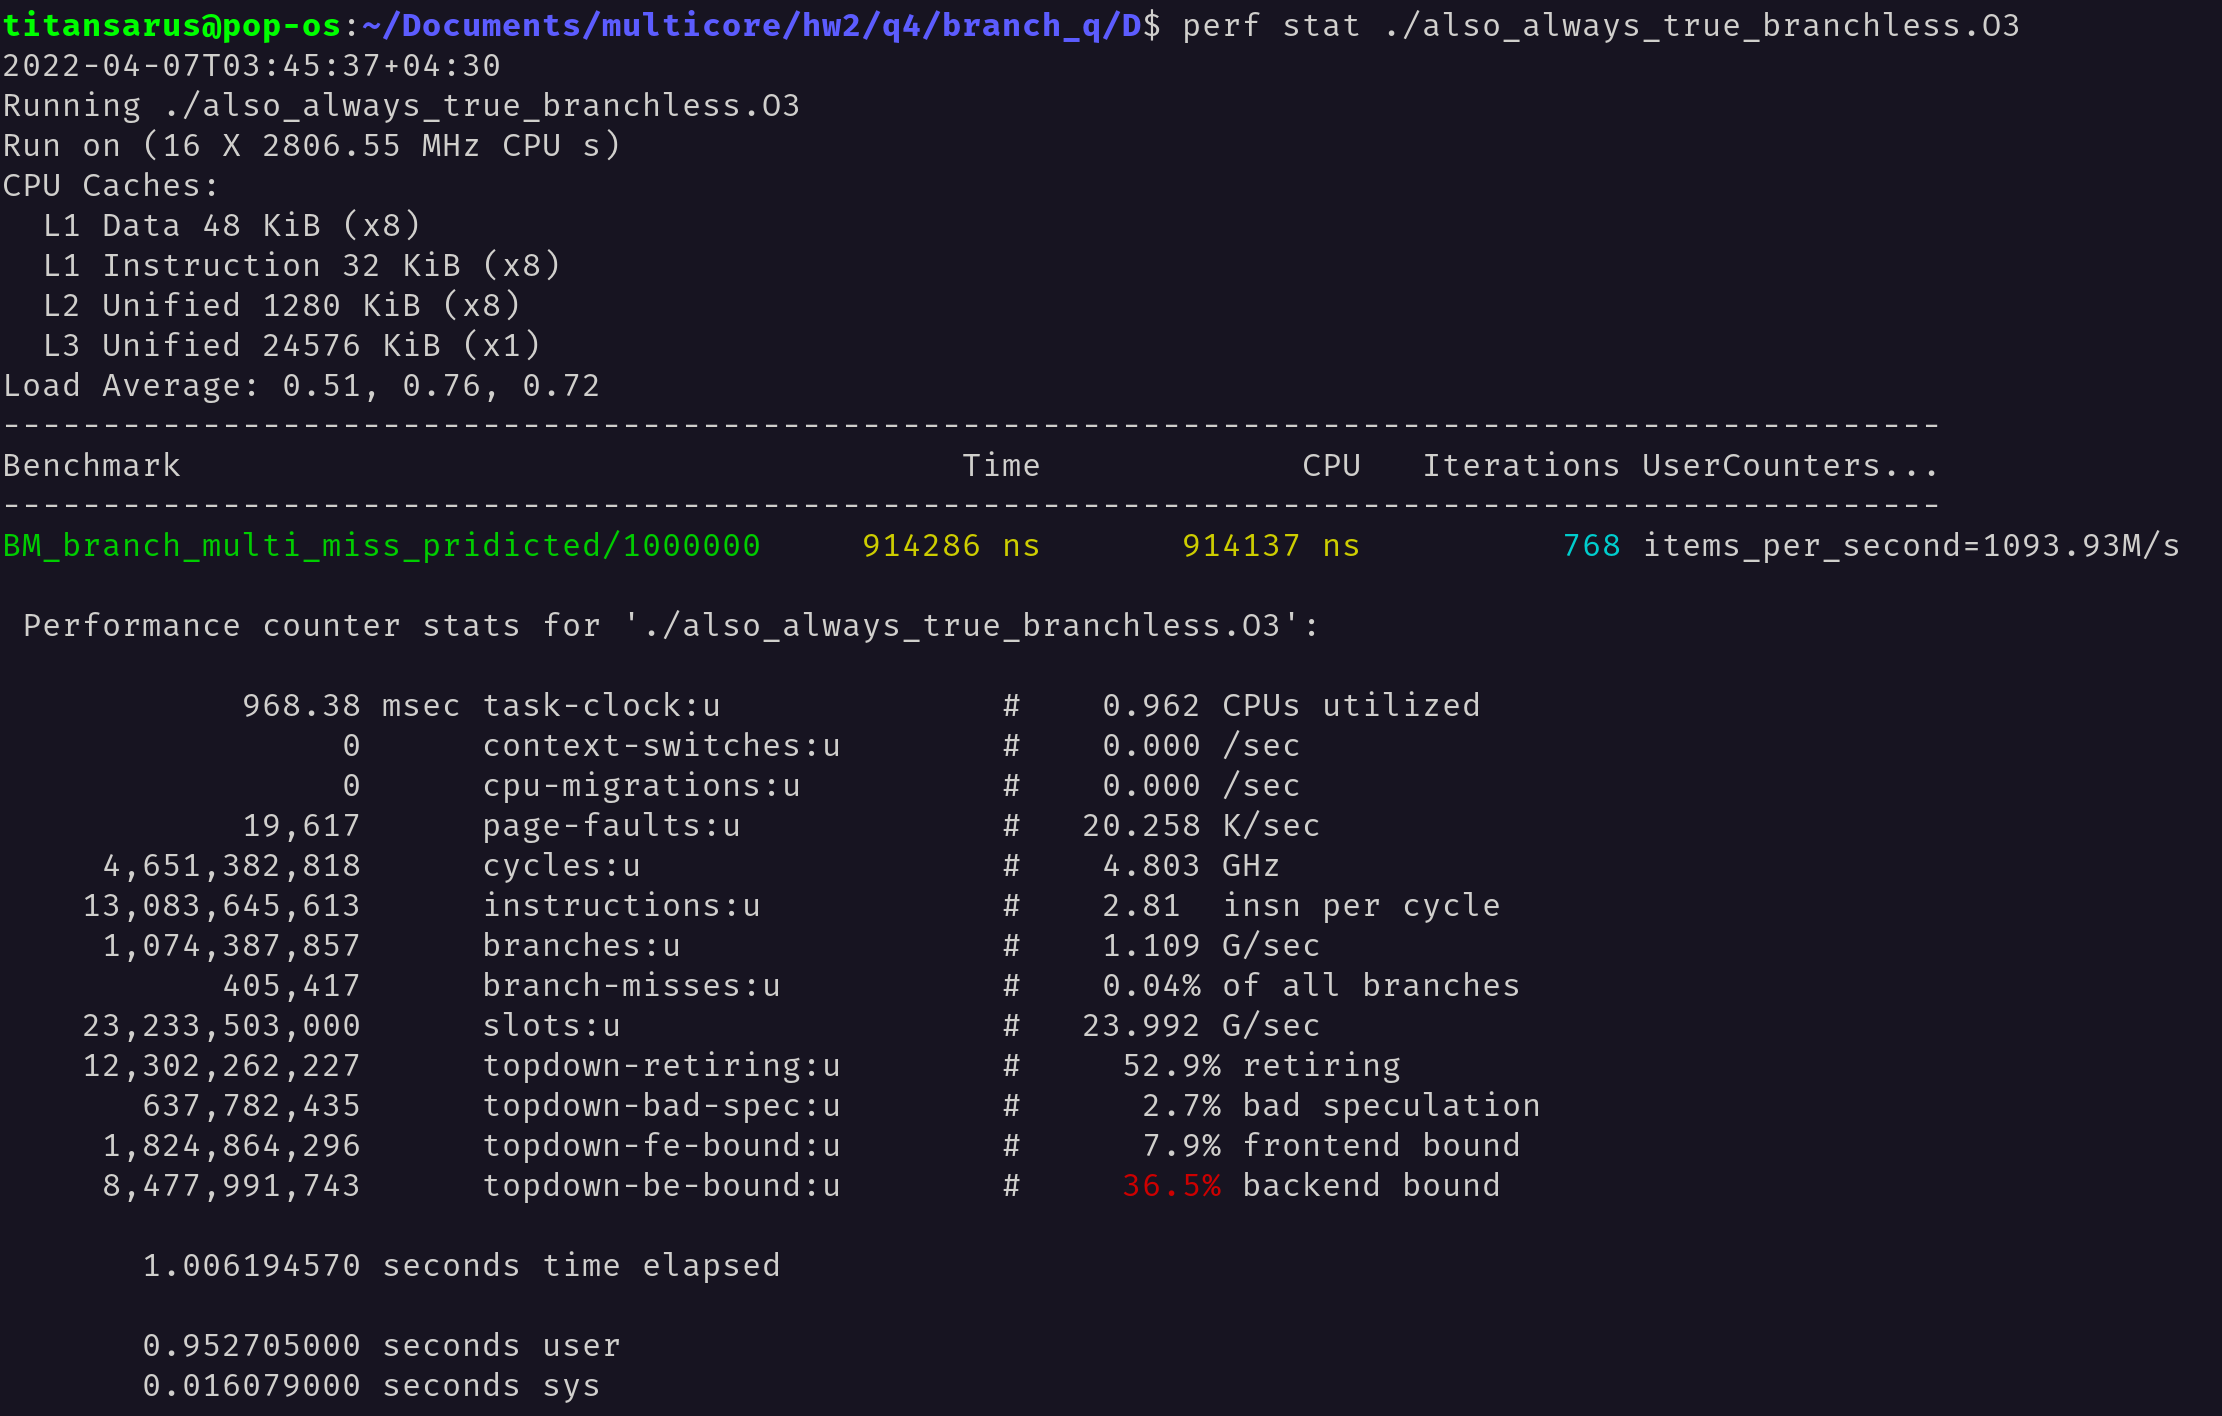
\includegraphics[width=0.75\textwidth]{./images/4D/also-always-true-b.png}	
	\cprotect\caption{\Verb+also_always_true_branchless.O3+}
\end{figure}

As it is evident in each case, we have a considerable performance boost by going branchless, and we see an increase in the number of iterations.
Also, we can see despite the massive increase in the number of iterations run, the overall number of branches didn't increase that much. It shows that most of the branches in the code are eliminated, and the minor increase in branch count is because of the huge increase in the overall iteration count. Also, we must note that \codeword{for} loops and the \Verb+benchmark+ library itself have branches, and we cannot eliminate all branches in the code, but we eliminated the main cause of branch counts.

\item 

There are two downsides to going branchless.
\begin{enumerate}
	\item Developer Experience: We usually replace the code with a more complex logic (complex in terms of human readability) by going branchless. This can lead to cases where the code is literally labeled as "Dark Magic," and no one ever dares to touch that code. This could reduce code modifiability and cause long debugging sessions if someone decides to touch that code without knowing what it does.
	
	This pops out another point in terms of developer experience, and it is the difficulty of implementing branchless logic in some cases. For example, making \codeword{||} conditions branchless needs the use of \codeword{|}. The caveat is that sometimes the condition operands have side effects. Maybe the code relied on short-circuit functionality to disable the side effect of the second operand in some cases. Still, by replacing \codeword{||} with \codeword{|}, we can cause this second operand's side-effect to kick in, and this could lead to problems. Getting these situations correct is, in many cases, tricky.
	
	\item Performance: By going branchless, especially in cases that have an \codeword{else} statement, causes our program to do more computations. In the cases above, this additional computation is not our performance bottleneck; the actual performance bottleneck was branches, and by eliminating that, we saw a huge performance boost. But in cases where computations are the bottleneck, going branchless could even lead to worse performance. We see such a case in the next part. 
\end{enumerate}
\end{itemize}
	
	\subsection{E}
	
	\begin{itemize}
		\item 
			Important parts of branchless Codes:
		
		
		\begin{lstlisting}[style=CStyle]
			//pure_random_branchless
			
            bool flag = (c_ptr[i] != 0);
a += ((flag) * (p1[i] + p2[i]) * (p1[i] + p2[i])) + ((!flag) * (p1[i] + p2[i]) * (p1[i] - p2[i]));
	//            if (c_ptr[i]) {
	//                a += (p1[i]+p2[i])*(p1[i]+p2[i]);
	//            } else {
	//                a += (p1[i]+p2[i])*(p1[i]-p2[i]);
	//            }
		\end{lstlisting}
		
		
		\begin{lstlisting}[style=CStyle]
			//predicted_branchless
			

bool flag = c_ptr[i] != 0;
a = (a + (flag) * p1[i]) * ((!flag) * p2[i] + (flag));
	//            if (c_ptr[i]) {
	//                a += p1[i];
	//            } else {
	//                a *= p2[i];
	//            }
		\end{lstlisting}
	
	\item 
	In the following pictures, you can see the output of \Verb+perf stat+ for of all files:
	
	\begin{figure}[H]
		\centering
		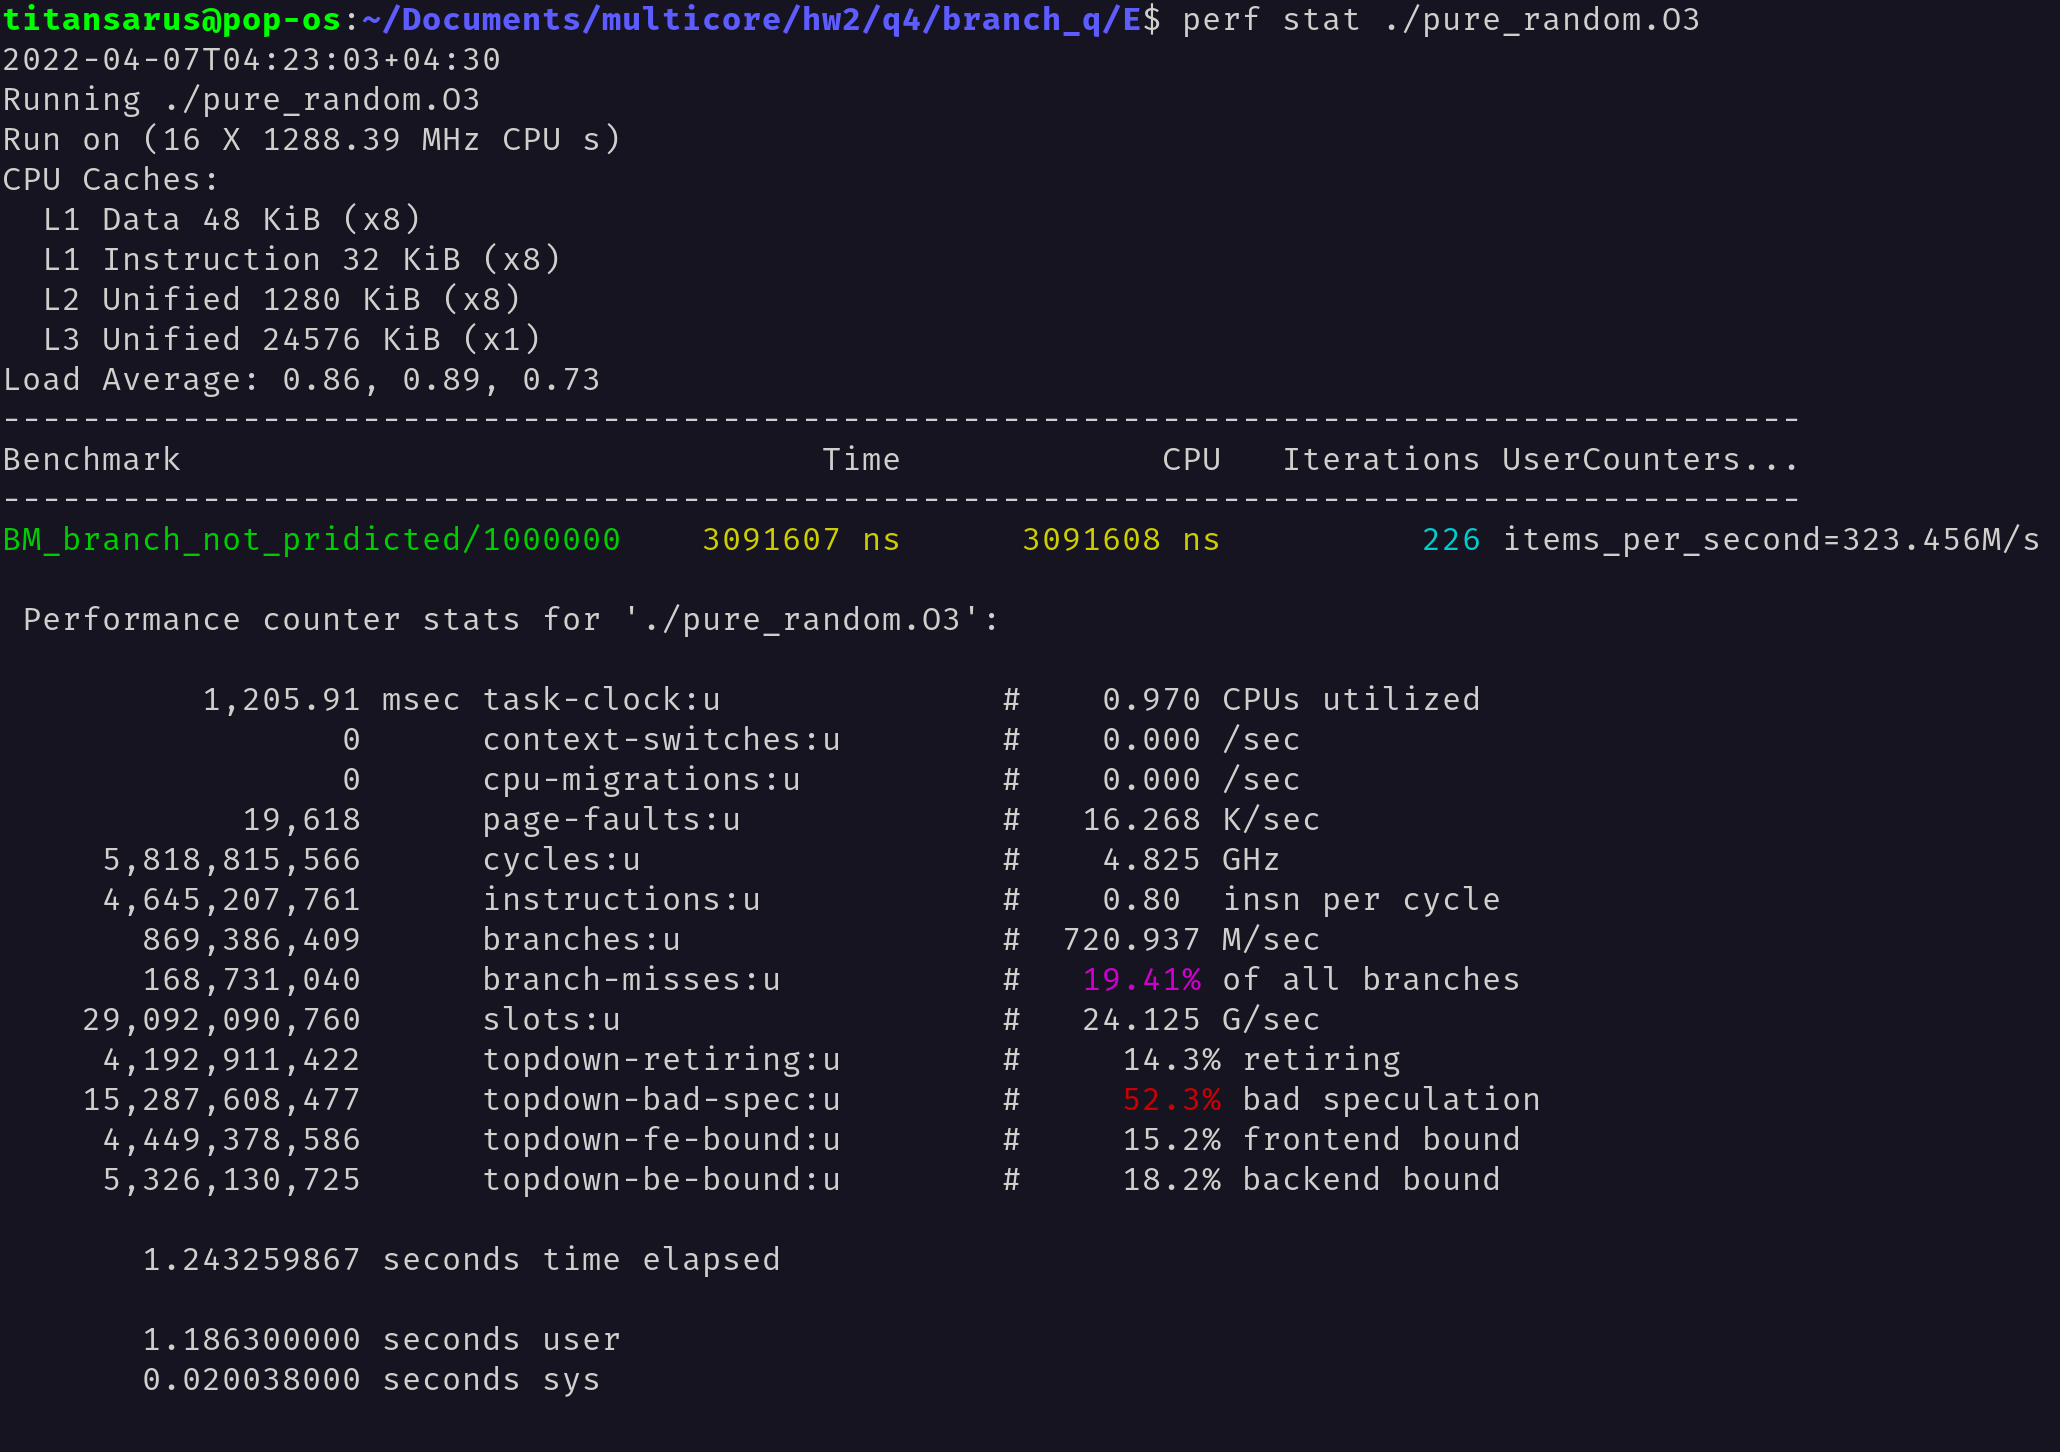
\includegraphics[width=0.75\textwidth]{./images/4E/pure-random.png}	
		\cprotect\caption{\Verb+pure_random.O3+}
	\end{figure}
	
	
	\begin{figure}[H]
		\centering
		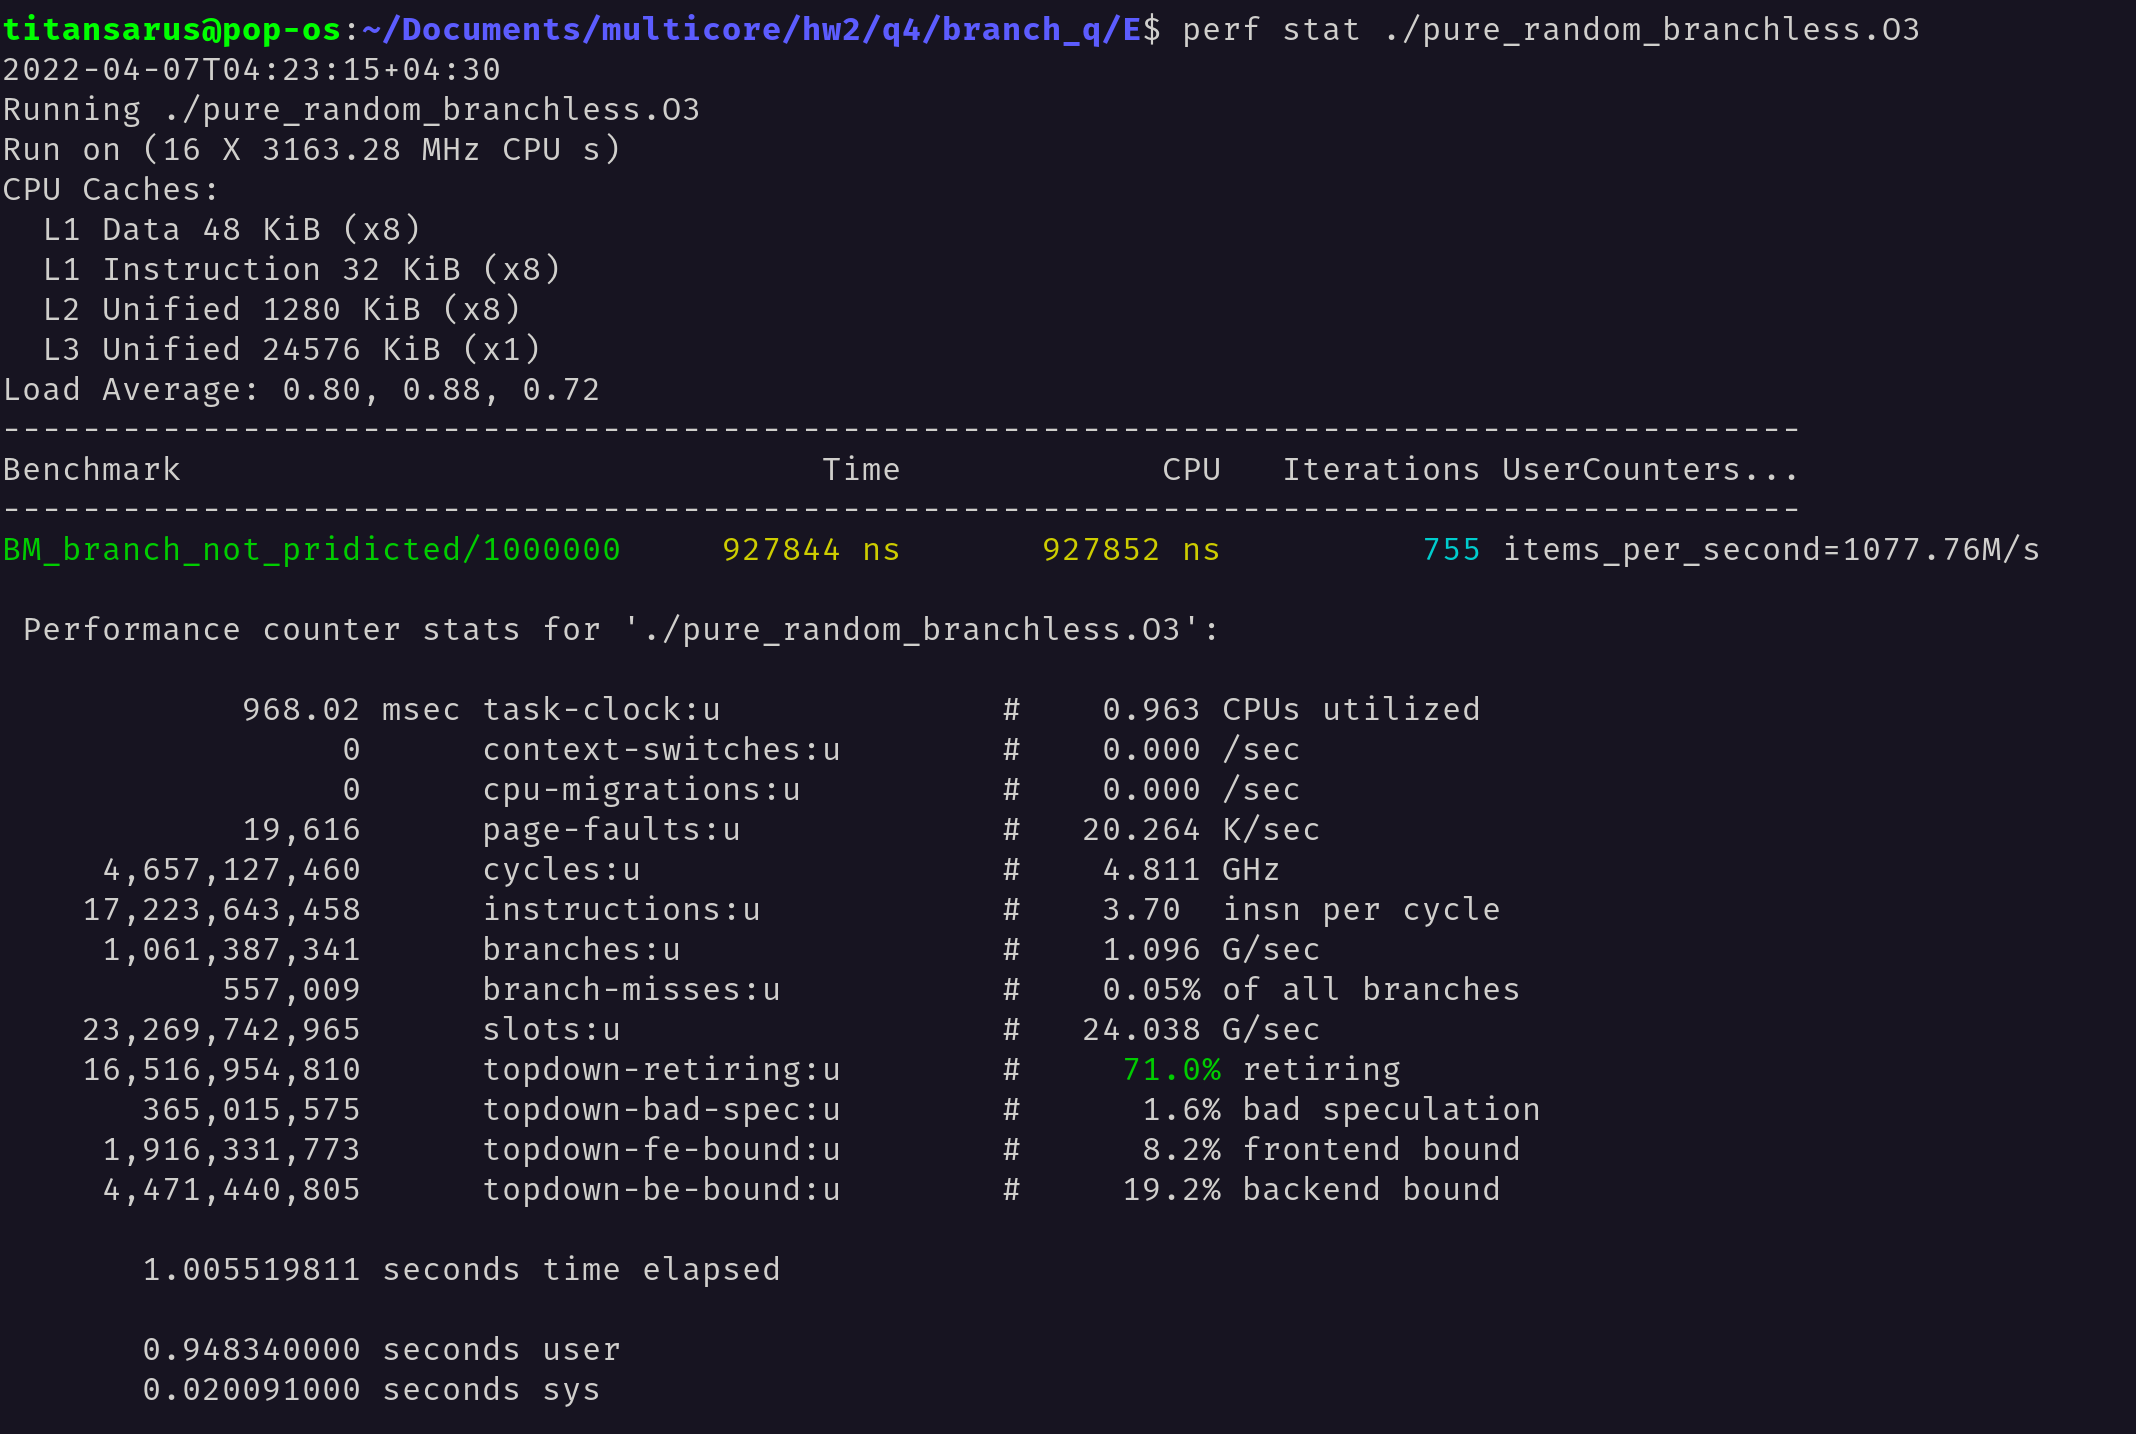
\includegraphics[width=0.75\textwidth]{./images/4E/pure-random-b.png}	
		\cprotect\caption{\Verb+pure_random_branchless.O3+}
	\end{figure}


	\begin{figure}[H]
	\centering
	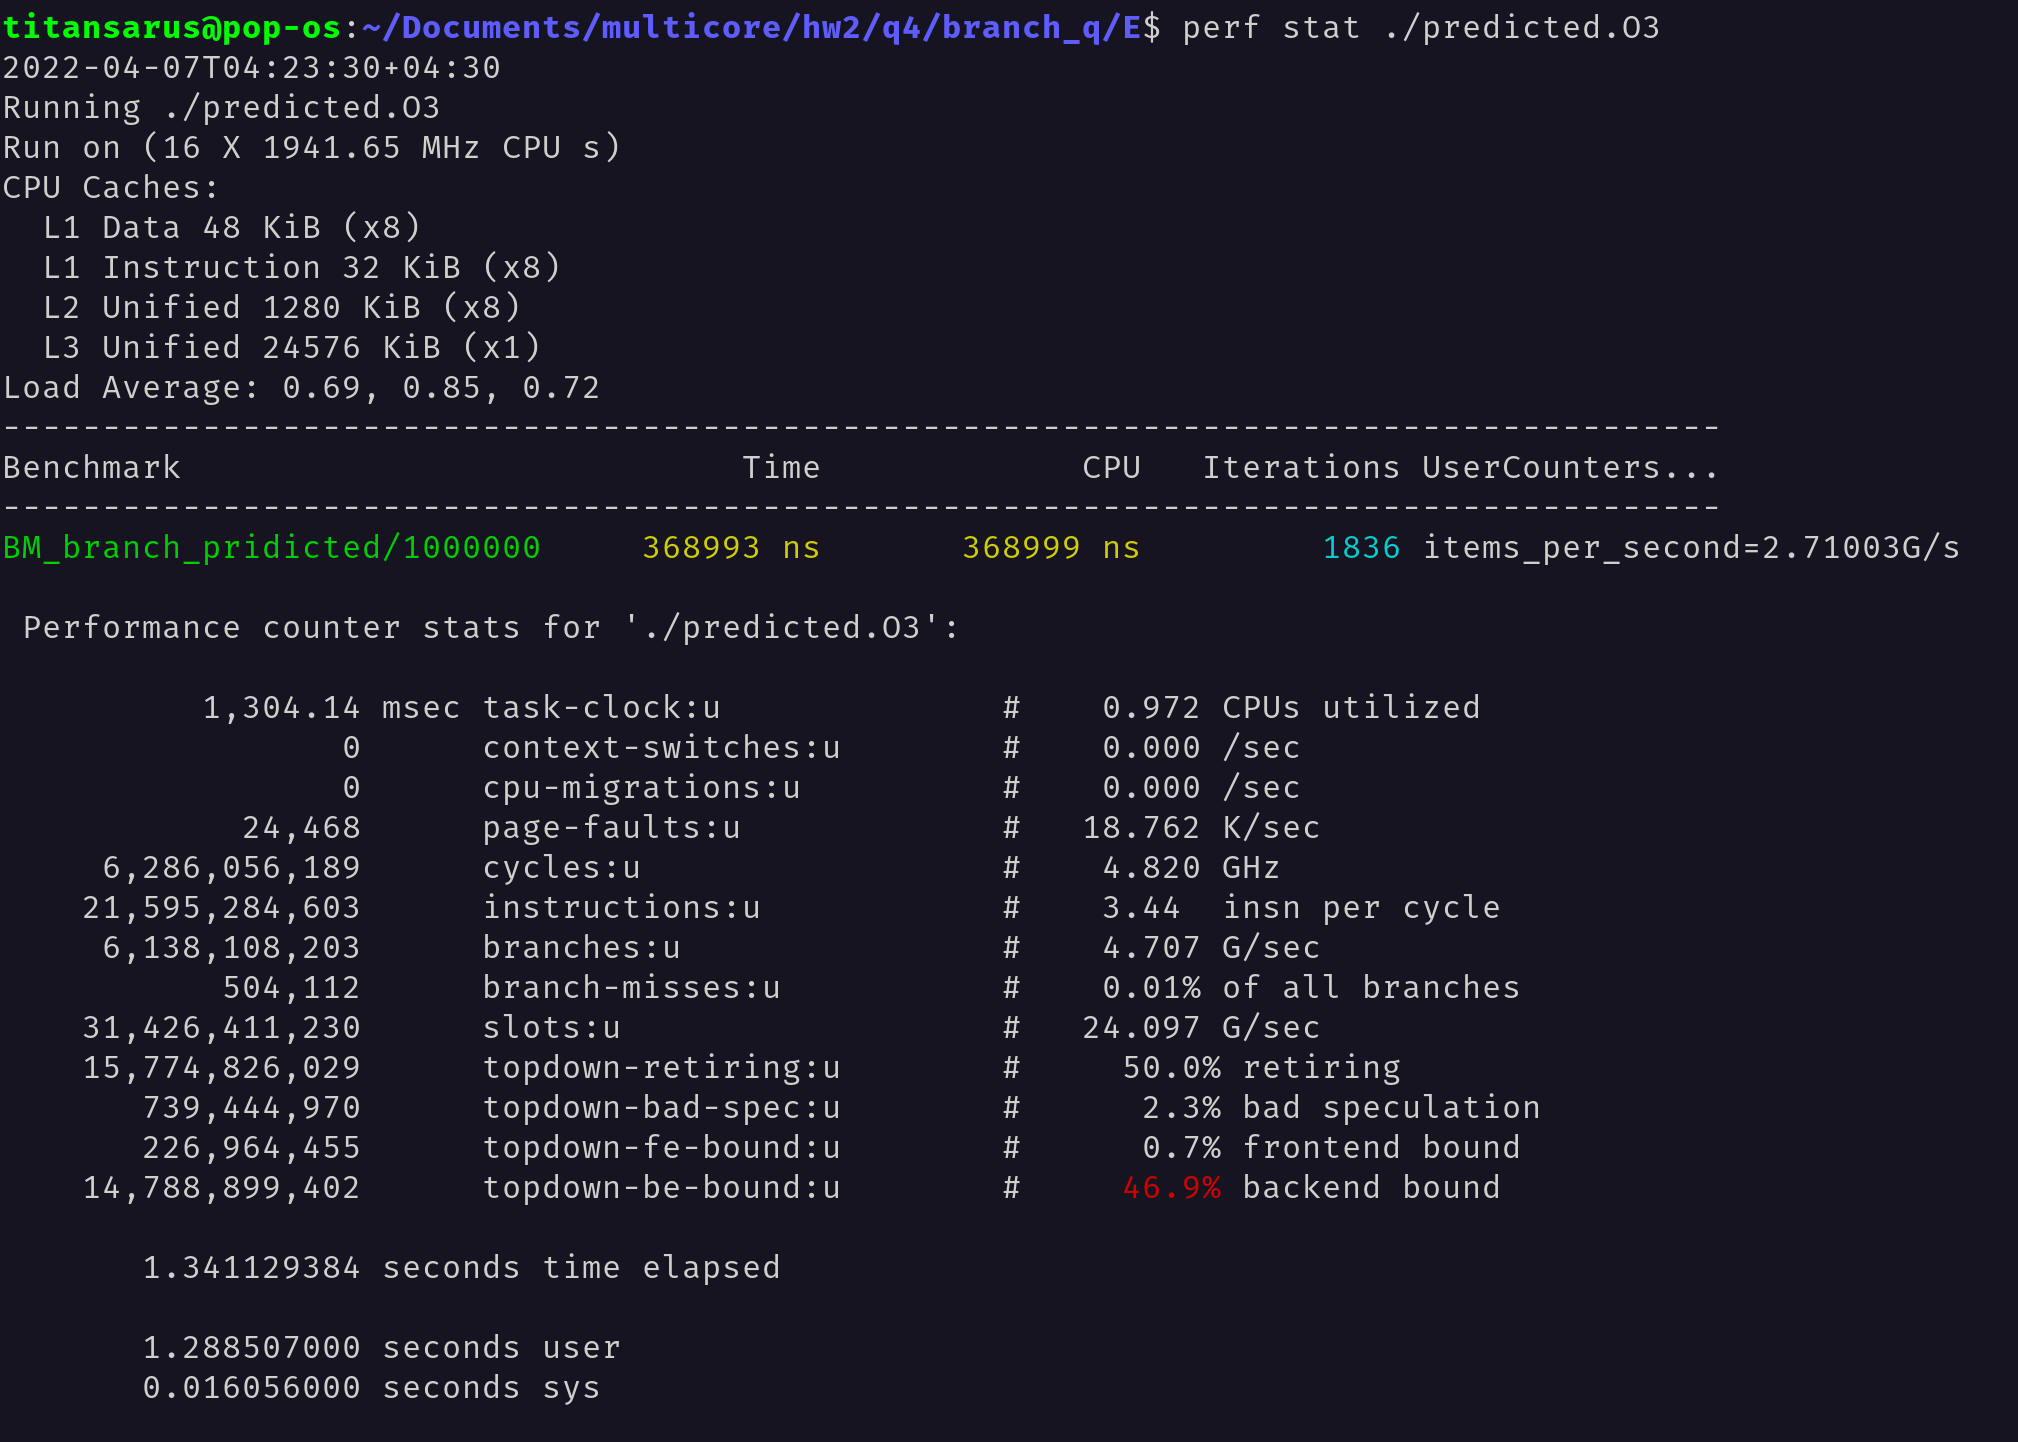
\includegraphics[width=0.75\textwidth]{./images/4E/predicted.png}	
	\cprotect\caption{\Verb+predicted.O3+}
	\end{figure}


	\begin{figure}[H]
		\centering
		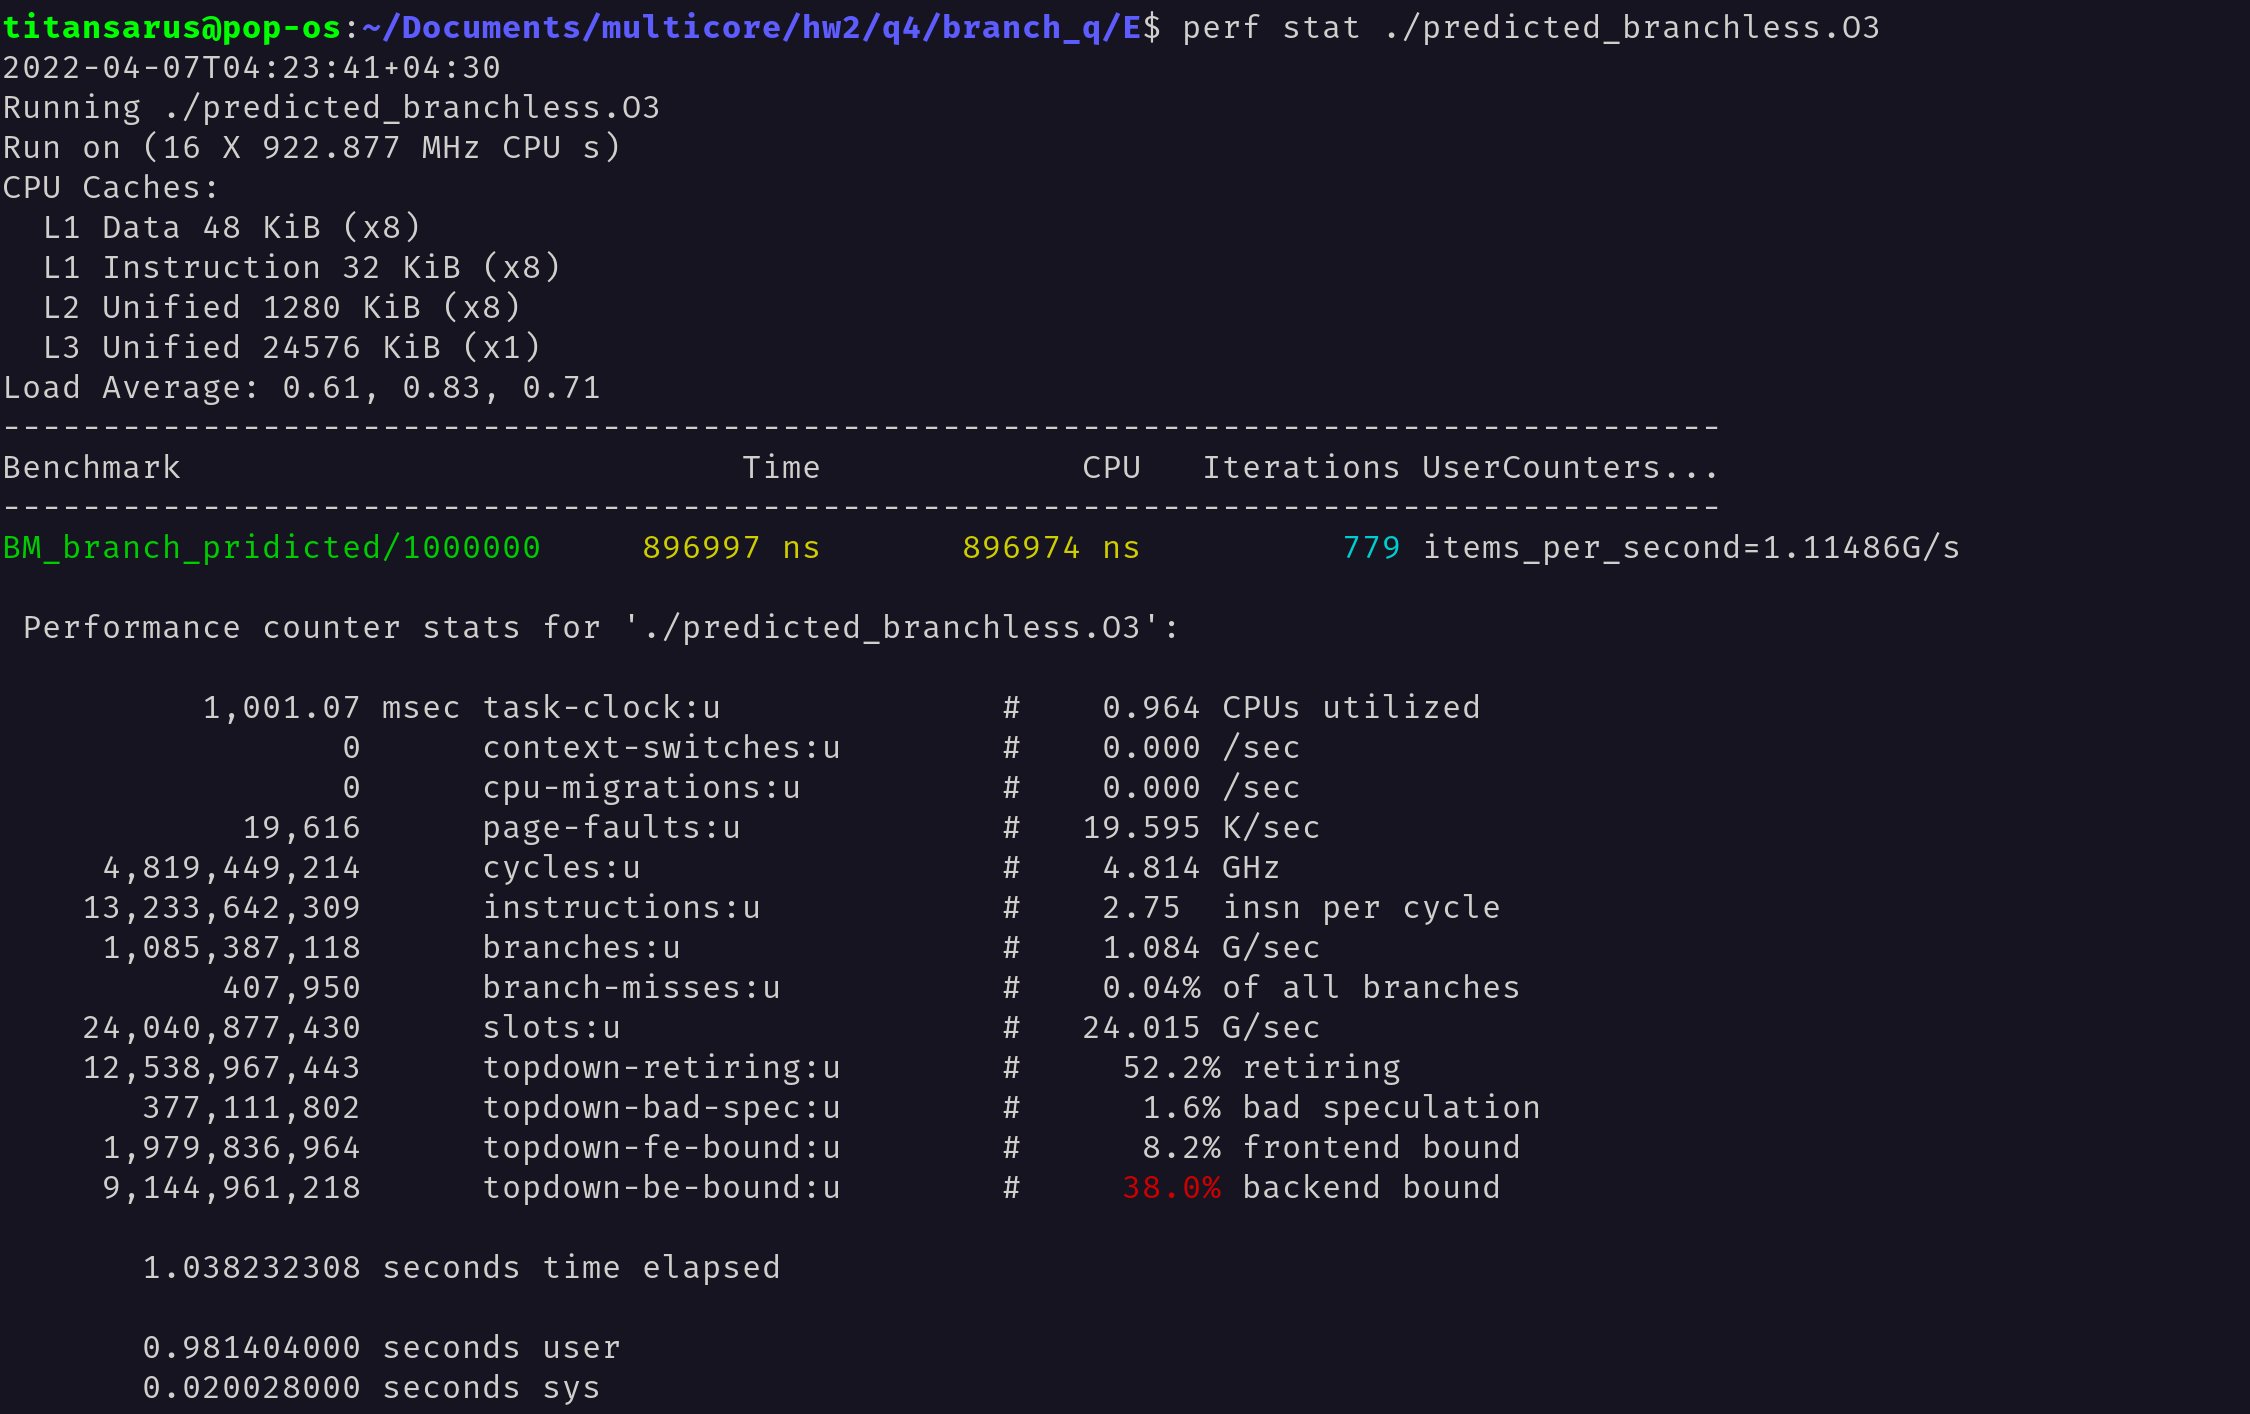
\includegraphics[width=0.75\textwidth]{./images/4E/predicted-b.png}	
		\cprotect\caption{\Verb+predicted_branchless.O3+}
	\end{figure}


\item 

The result for \Verb+pure_random+ is as expected, and it had a considerable performance boost. But we can see a decrease in performance for \Verb+predicted+.

This is because the main bottleneck in \Verb+pure_random+ is the branches. We see a huge amount of branch misses in the non-branchless case. Making it branchless decreases this branch misses by a large margin and causes a performance boost.

It is not the case for \Verb+predicted+. Even the not-branchless version doesn't have lots of branch misses. It follows a simple "always true" pattern for the branch, and the CPU's branch predictor could easily predict it right. By making it branchless, we cause an increased computational overhead for the program. It should now always compute the multiplication part (\codeword{else} part of the condition) regardless of the actual value of the flag. This increase in computations also occurred in \Verb+pure_random+, but in that case, the main bottleneck was branch misses, and eliminating them gives us more performance than what the increase in computations takes from us. But in \Verb+predicted+ case, we didn't have that type of bottleneck on branches, and even having the branch caused the CPU to ignore the multiplication part; Therefore, by going branchless, we force the CPU to do useless arithmetic computations in each round and therefore, the performance decreased.
	
		\end{itemize}
	
	\subsection{F}
	
	
	\begin{itemize}
	\item 
	As we saw in part A, the compiler optimizes branches when it can deduce the result of the condition with confidence. Suppose the result of the condition is a constant expression or a call to a function that returns an easily predictable value (For example \codeword{1}). In that case, the compiler can optimize the branch out.
	
	In other cases, for example, when we have memory access, the compiler doesn't do very much in terms of optimizing the branch. 
	
	There can be other ways of optimizing branches. For example, \Verb+gcc+ can use some heuristics to guess the result of the branch and give CPU hints about its possible result, but we didn't cover these cases in this question.
	
	
	\item 
	Based on the CPU, there could be different branch predictors. But most modern CPUs, including the one we used in this question, seem to at least implement some sort of history-based pattern recognition predictors. For example, consider the case of $001001001001\cdots$ for a branch condition. In this case, the CPU's branch predictor will predict a one after seeing two zeroes and a zero after seeing $01$. In part B, we saw something similar. CPU's branch predictor quickly recognized $10101010\cdots$ pattern and predicted it in such a way that we almost see no significant branch miss.
	
	It is noteworthy that some more complex mechanisms could be built into the actual modern CPUs. For example, Ryzen CPUs use some sort of neural network to predict the result of branches.
	
	But as a general answer, the CPU considers the "History" of previous branch results when predicting branches.
	
	\item 
	
	
	The CPU is good at branches that follow a pattern. The more well-defined the pattern is, the better the CPU will predict. It will easily predict "Always True" or "Alternating" patterns, but it probably cannot predict the "Prime number" pattern.
	
	Also, the CPU is good at predicting each branch, but it cannot easily predict the relation between branches.
	
	\item 
	The CPU could not perform well for interdependent branches whose relation may not be obvious.
	
	For example, we saw the \codeword{condition1 || condition2} cases, in which the compiler generates two branches. In the example, we saw that the conditions were the logical opposite of each other, but the CPU could not find this inter-branch pattern, and because each branch followed a random pattern, the CPU was not good at predicting the result.
	
	
	\item 
	We should use branchless in performance-critical codes in which branches are a critical bottleneck. In cases where the CPU would probably predict branches pretty well, branchless programming is pointless and could have negative results. Especially in cases where each part of the branch is somewhat computationally intensive, making the code branchless could cause these computations to run in any case, so removing the branch should be higher than this increase in computation cost if we want to use branchless programming.
	
	Also, generally in non-performance-critical codes, and in cases where readability is more important than performance, it is better to avoid branchless programming because it could lead to more complex logic on the developer side.
	
	
	
	
	\end{itemize}
	
	
	
	\newpage
	


\end{document}



